\chapter{Część praktyczna}
Cykl życia standardowej strony internetowej przedstawiono na rysunku \ref{fig:rysunek_7}

\begin{figure}[!ht]
    \centering
    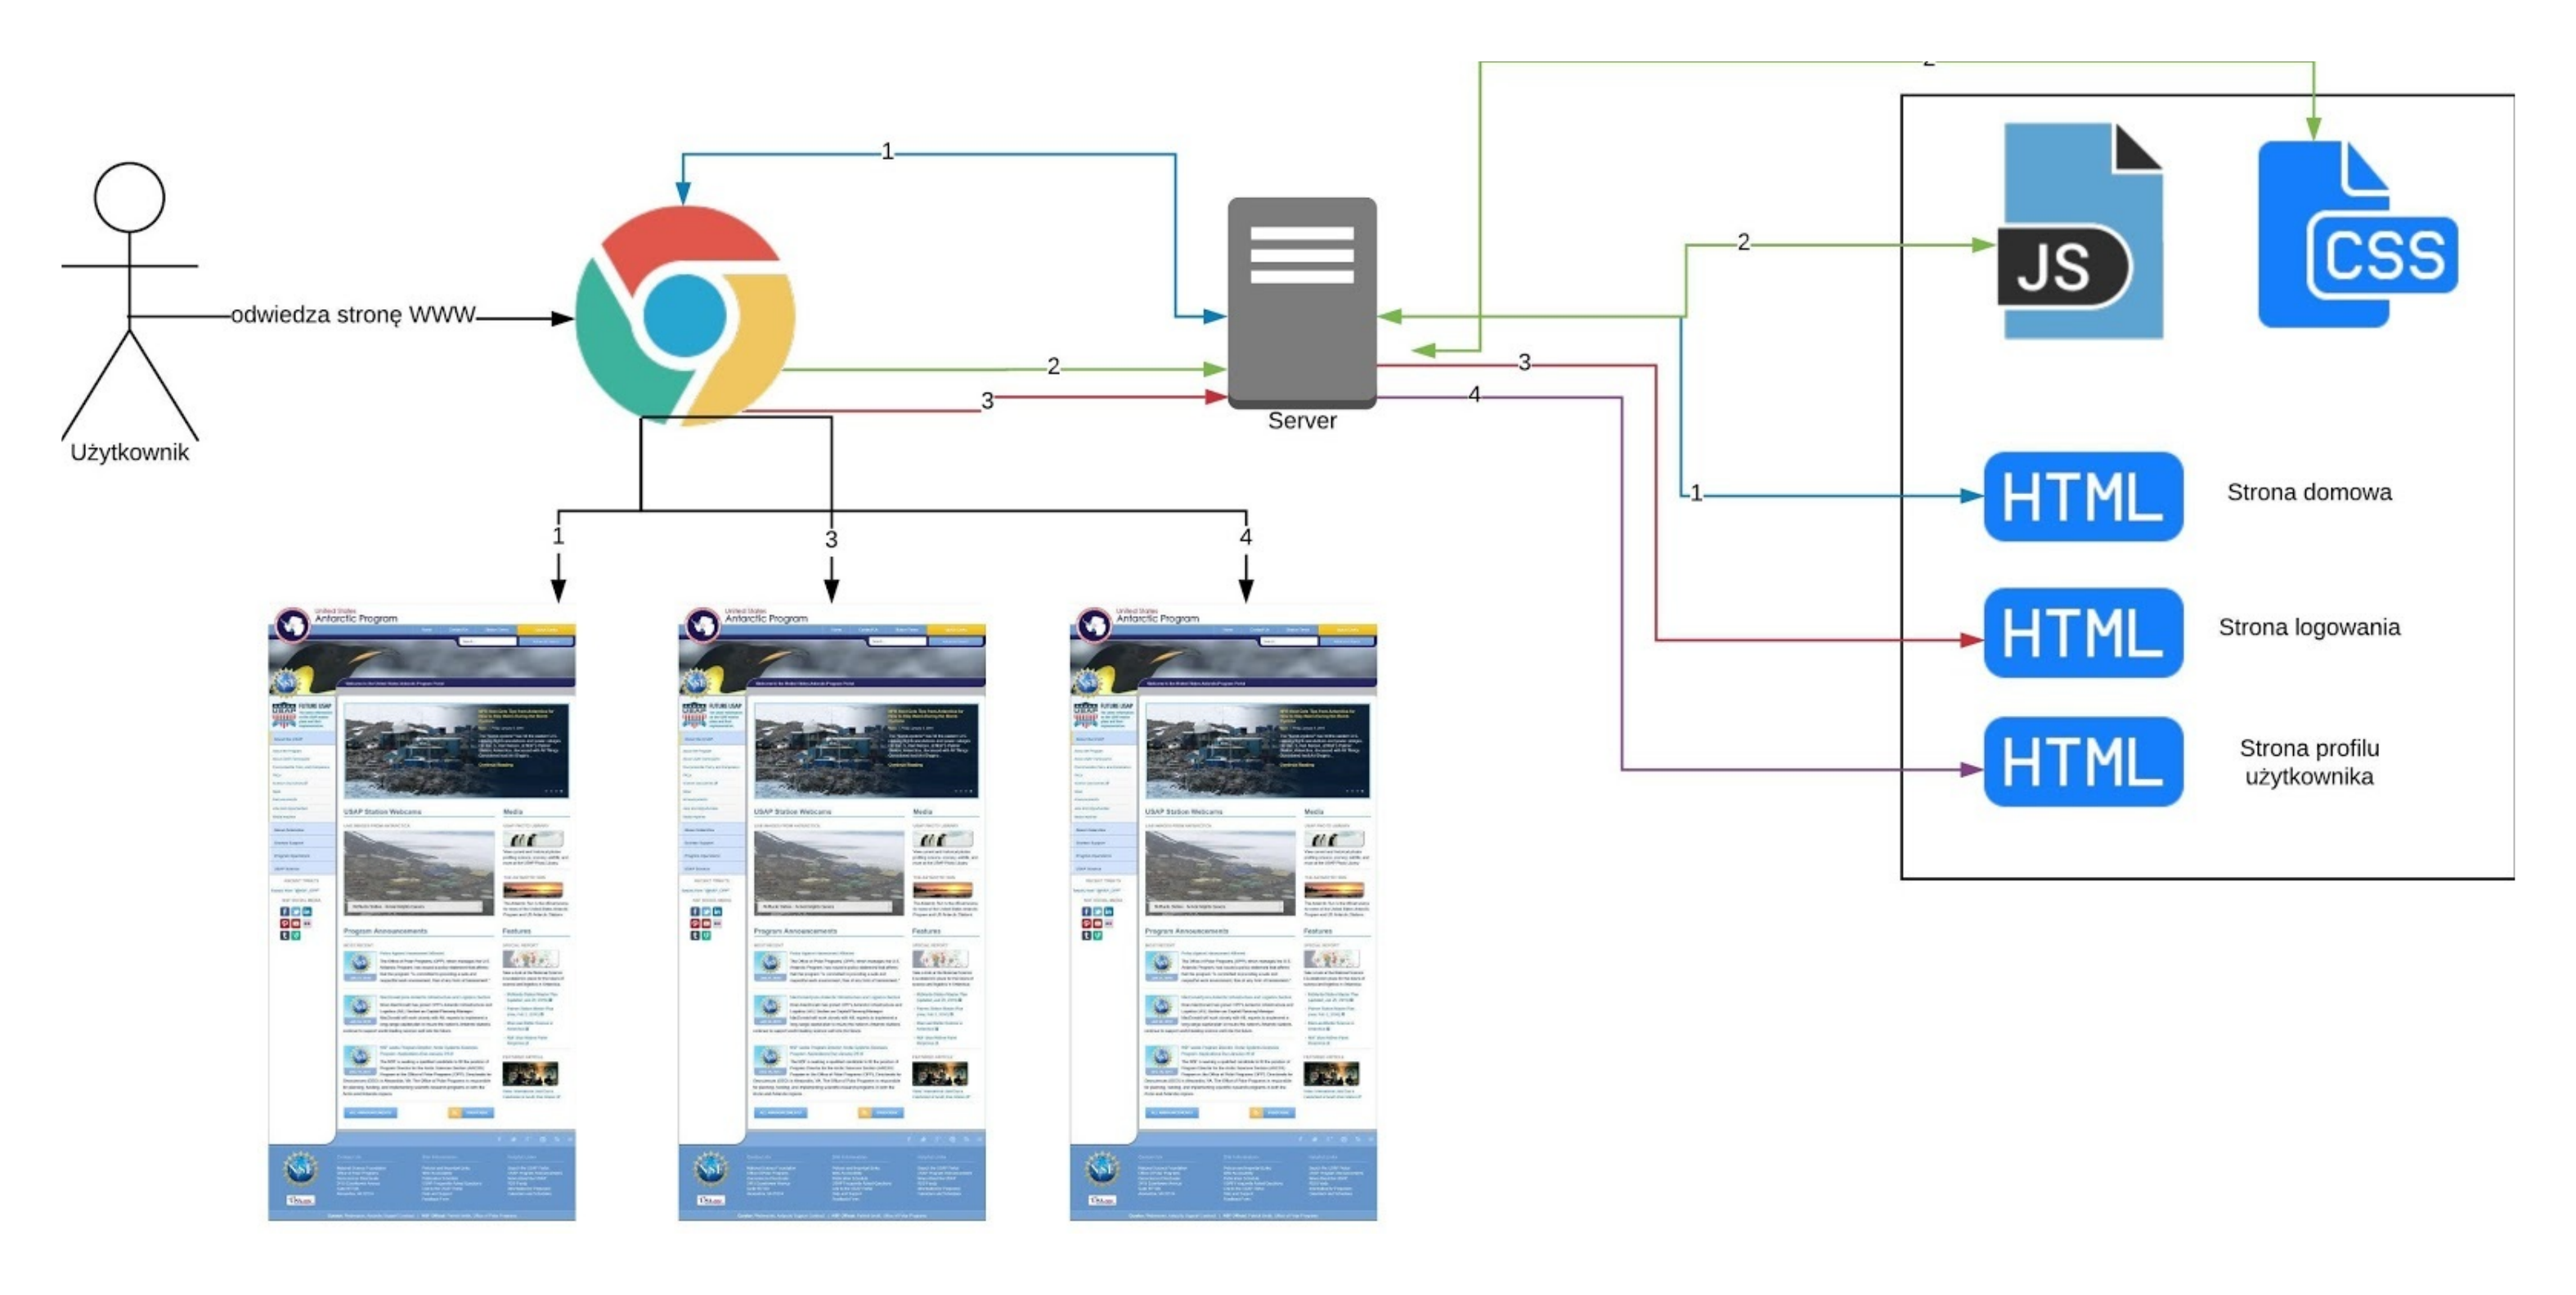
\includegraphics[width=12cm]{rysunek_7.png}
    \caption{Ilustracja przedstawiająca cykl życia statycznej strony internetowej}
    \label{fig:rysunek_7}
\end{figure}

\begin{itemize}
	\item Użytkownik otwiera przeglądarkę i odwiedza stronę WWW.
    \item Przeglądarka wysyła zapytanie do serwera z żądaniem zasobów.
    \item Serwer odsyła plik HTML w którym znajdują się odnośniki do plików JavaScript oraz CSS.
    \item Przeglądarka pobiera pliki JavaScript oraz CSS
    \item Przeglądarka renderuje stronę dla użytkownika.
    \item Użytkownik klika w odnośnik do kolejnej strony ( w przykładzie strona logowania)
    \item Przeglądarka pobiera cały nowy plik HTML
    \item Przeglądarka renderuje nową stronę od nowa.
    \item Przeglądarka ponownie pobiera dodatkowe pliki JavaScript oraz CSS (zakładamy, że przeglądarka nie przechowuje plików w pamięci podręcznej).
    \item Przeglądarka renderuje stronę od nowa.
\end{itemize}

Jak widzimy, cały proces odwiedzenia dwóch stron w tej samej domenie wymaga każdorazowego przeładowania strony oraz pobrania tych samych danych.
Proces ten wymaga ciągłego pobierania plików HTML, pobierania plików dodatkowych co obciąża procesor, pamięć łącze oraz sam serwer.

Dla porównania, przedstawiona poniżej ilustracja pokazuje cykl działania aplikacji SPA (rysunek \ref{fig:rysunek_8})

\begin{figure}[!ht]
    \centering
    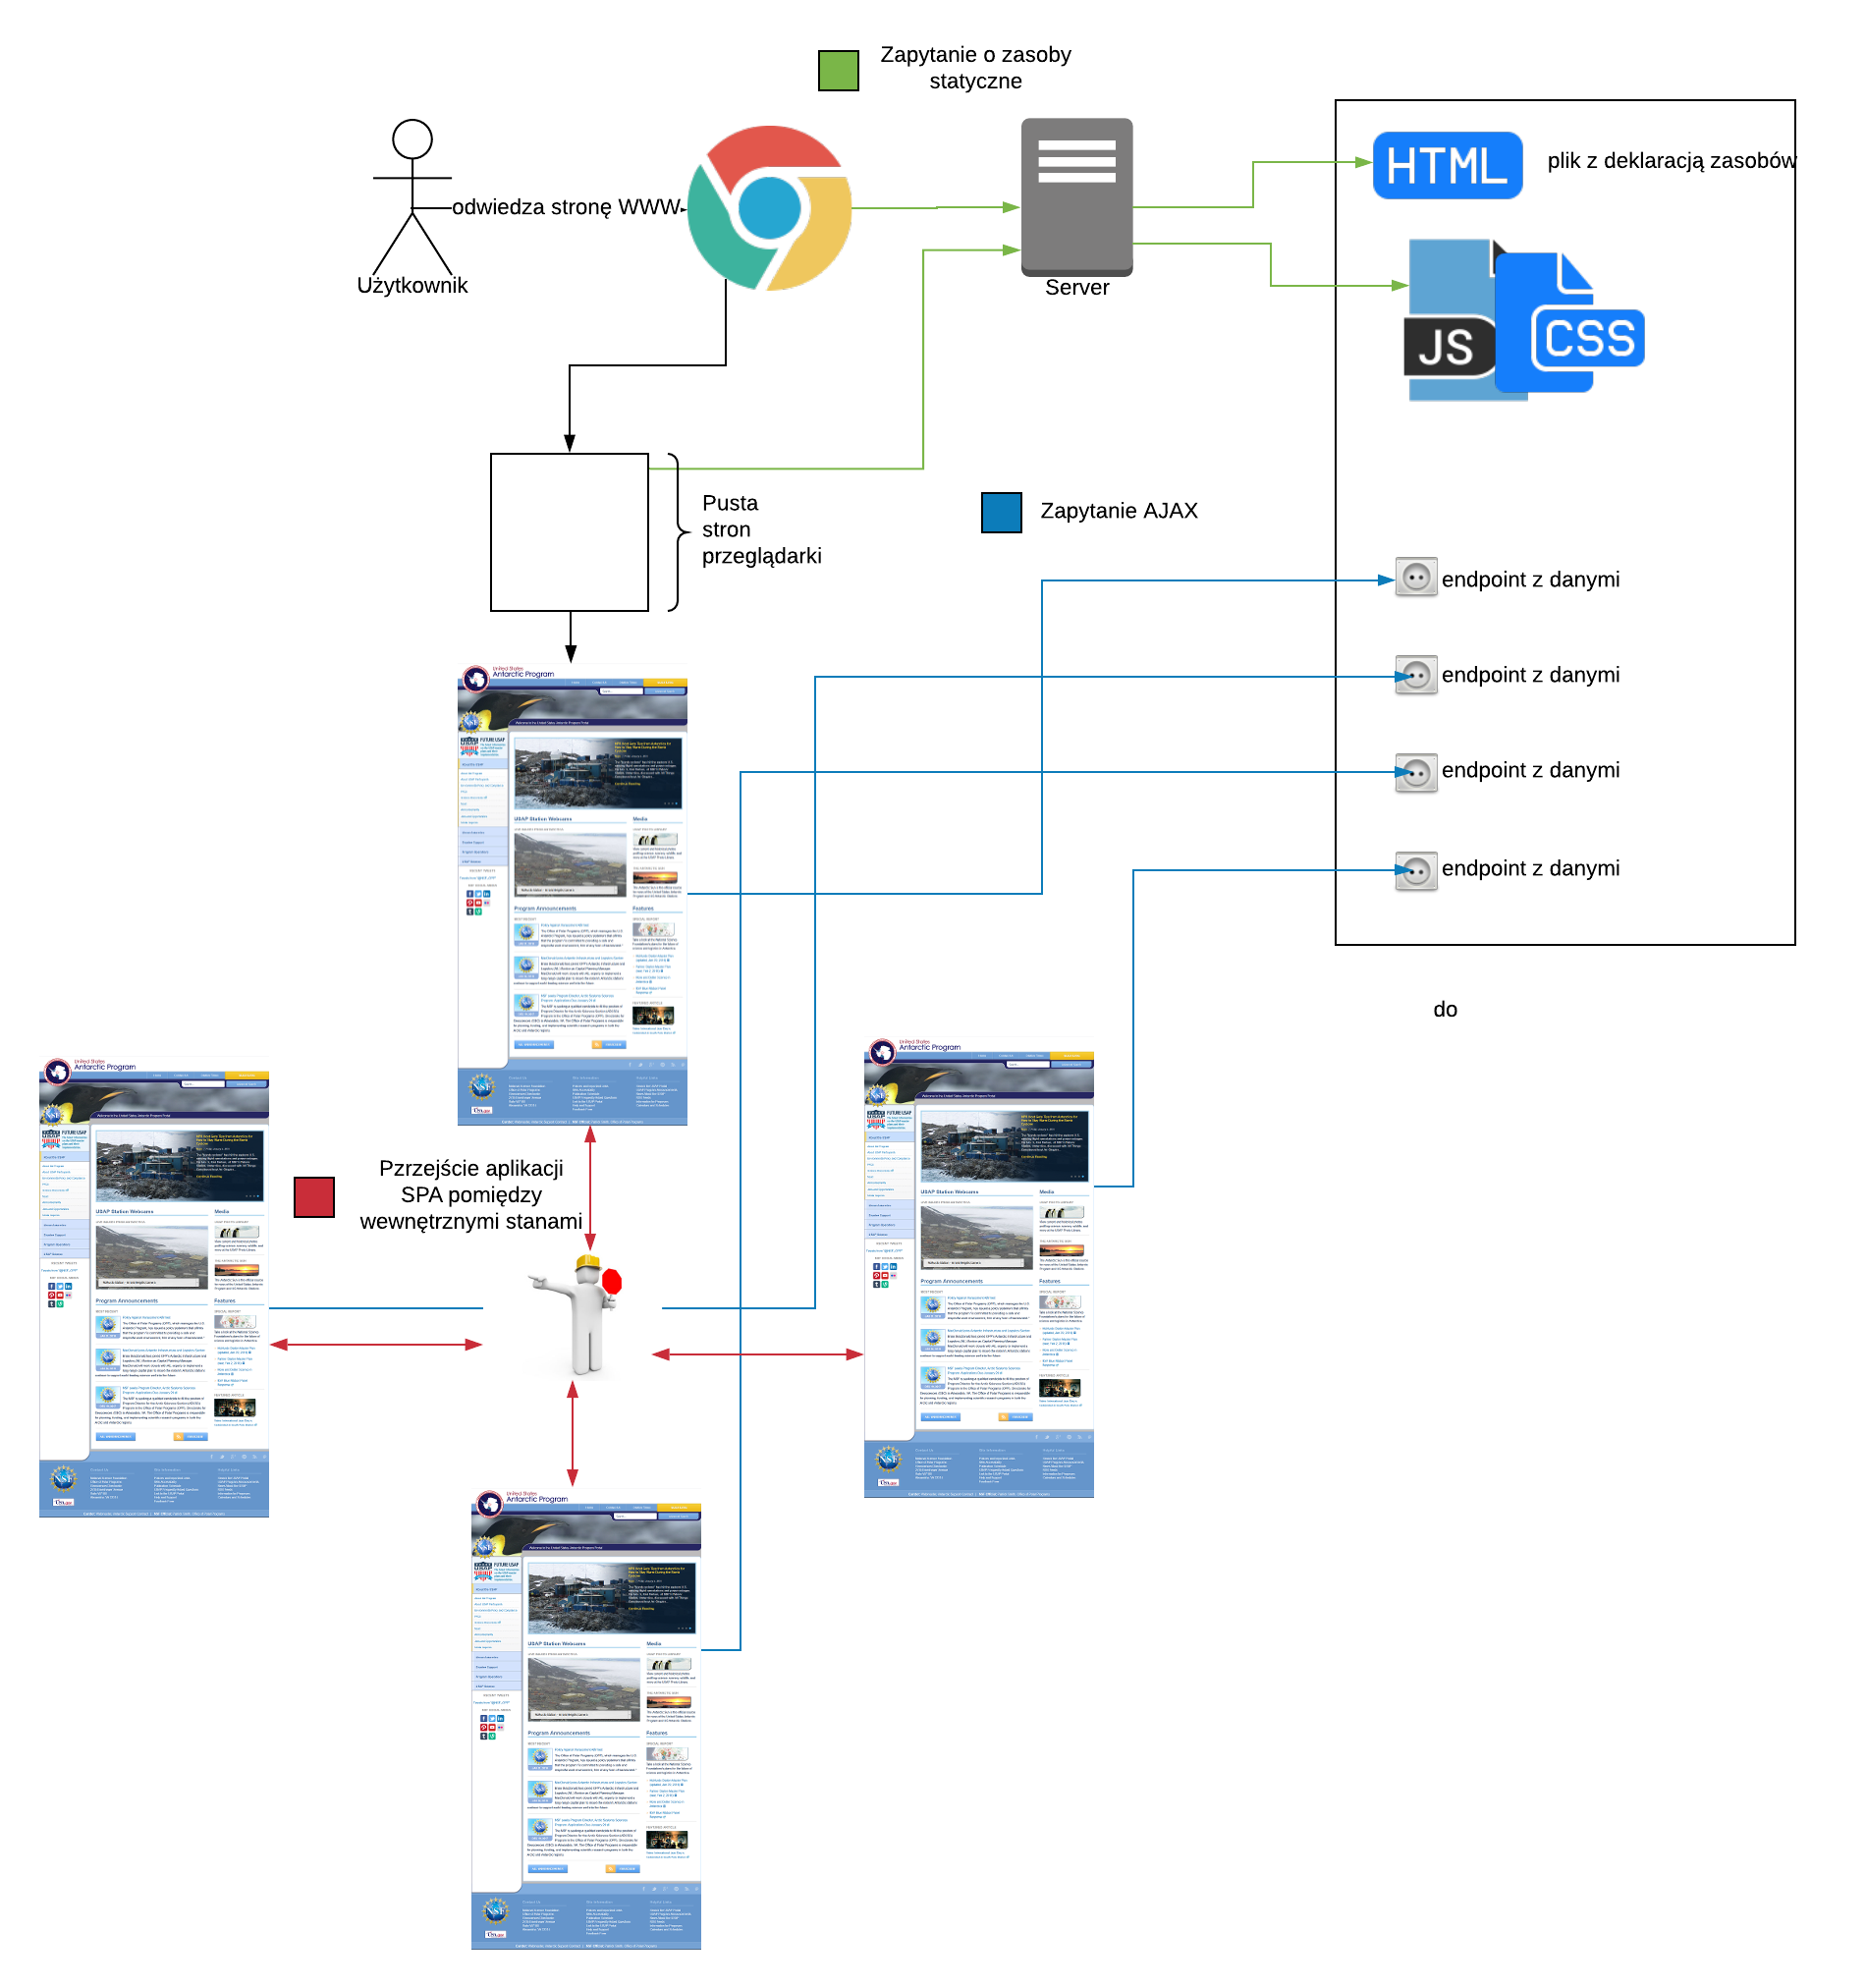
\includegraphics[width=12cm]{rysunek_8.png}
    \caption{Ilustracja przedstawiająca cykl działania aplikacji SPA}
    \label{fig:rysunek_8}
\end{figure}

\begin{itemize}
    \item Użytkownik odwiedza tę samą stronę .
    \item Przeglądarka pobiera plik HTML z definicją potrzebnych zasobów. Zazwyczaj sekcja body pliku jest pusta.
    \item Przeglądarka pobiera dodatkowe pliki JavaScript oraz CSS.
    \item Często pliki te są zoptymalizowane poprzez kompresję i sklejone w jeden plik tak, aby wykonać tylko jedno zapytanie zamiast dwóch.
    \item Pliki JavaScript, generują treść strony HTML.
    \item Przeglądarka może ( ale nie musi ) wykonać dodatkowe zapytanie o dane do jednego z endpointów serwera.
    \item Użytkownik klika na odnośnik do kolejnej strony. Przeglądarka nie pobiera już dodatkowego pliku HTML, jako, że aplikacja jest dynamiczna. Skrypt JavaScript może, ale nie musi pobrać dodatkowych informacji z serwera.    
\end{itemize}

Jak widzimy, wykonano znacznie mniej zapytań do serwera. Dodatkowe zapytania które skrypt może wykonać w celu pobrania danych zazwyczaj są znacznie mniejsze od pełnego pliku HTML z wybraną treścią.
Dodatkowo, przeglądarka nie przeładowuje strony przy każdej zmianie podstrony, co także odciąża procesor jak i łącze sieciowe.

\section{Problem pomiaru wydajności aplikacji SPA}

Z racji, że w aplikacjach SPA nigdy nie następuje przeładowanie strony, a ich działanie jest ciągłe pojawia się problem następującej natury. 

W celu ułatwienia zrozumienia problemu posłużę się przykładem przedstawionym na rysunku \ref{fig:rysunek_9}. Załóżmy że jesteśmy na platformie Netflix. Otworzyliśmy stronę z listą dostępnych filmów do obejrzenia. 

\begin{figure}[!ht]
    \centering
    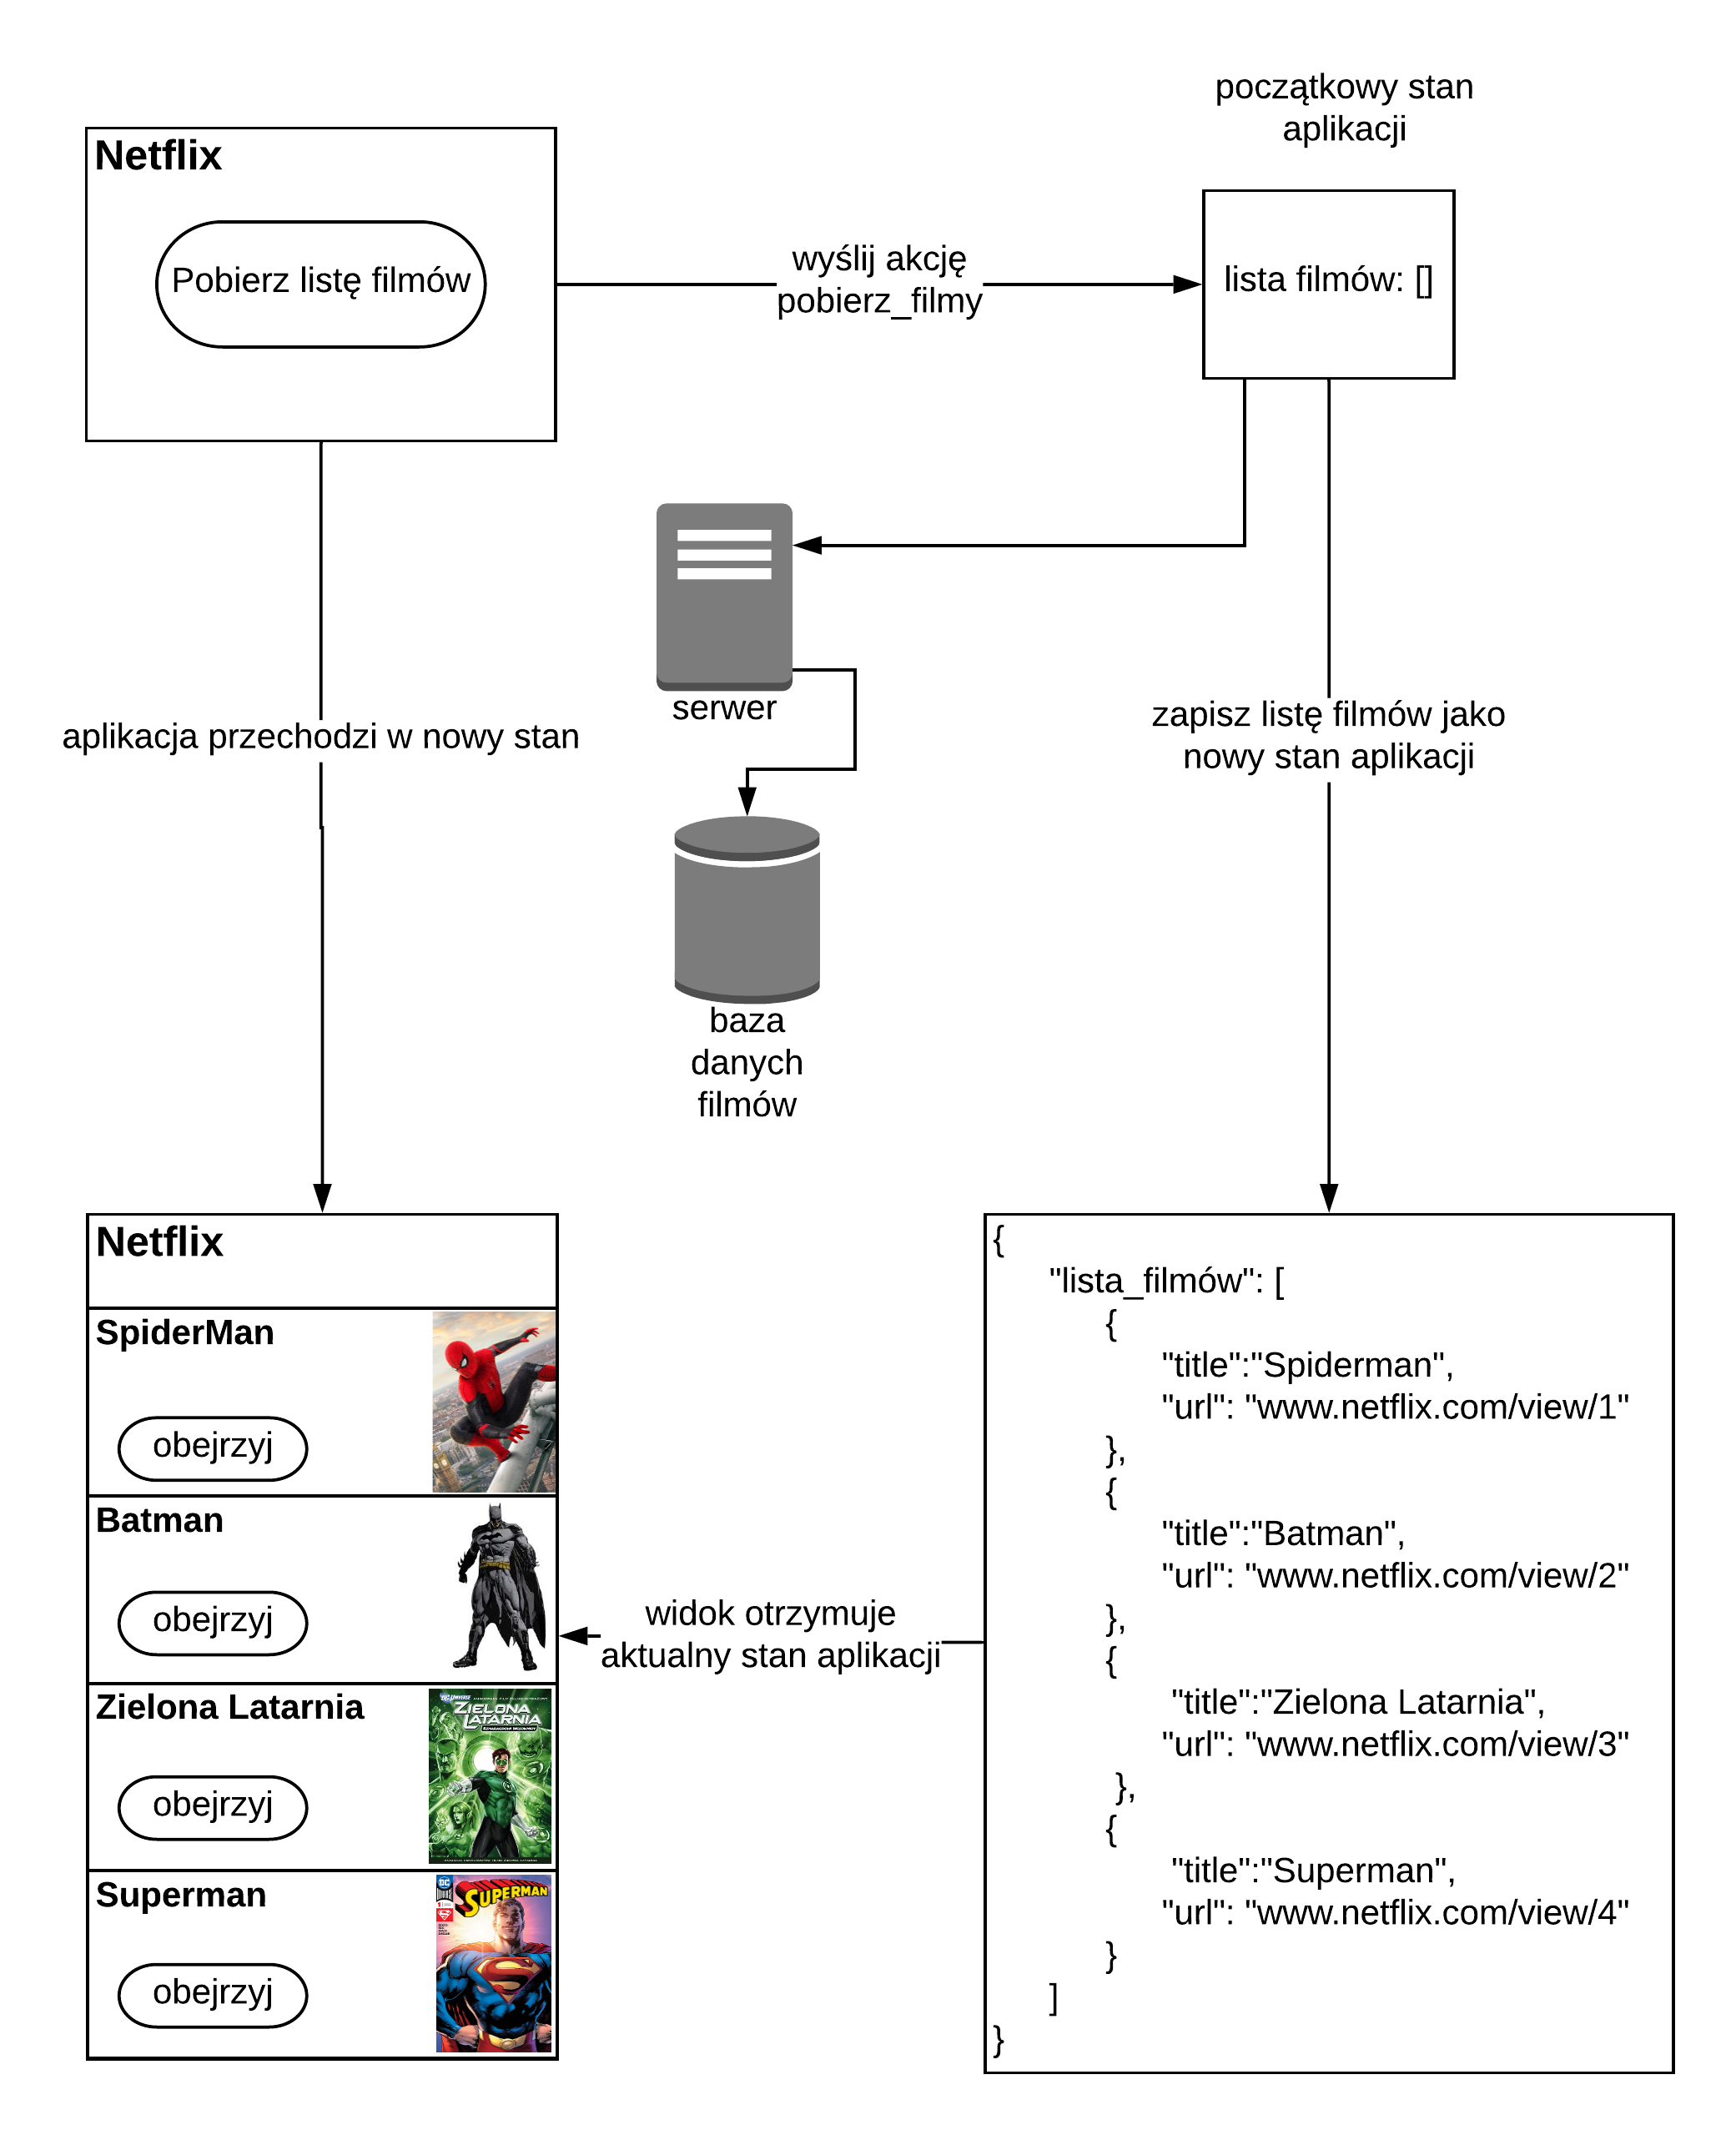
\includegraphics[width=12cm]{rysunek_9.png}
    \caption{Grafika przedstawiająca mechanizm działania aplikacji dynamicznych}
    \label{fig:rysunek_9}
\end{figure}

Aplikacja w stanie początkowym nie posiada żadnych filmów. Użytkownik klika przycisk pobierz listę filmów. Efektem ubocznym (side effect)  jest wysłanie informacji o akcji do menedżera stanu.
Menedżer stanu wysyła zapytanie do serwera o listę filmów do zaproponowania. Serwer odpowiada z danymi, i menadżera stanu przechodzi w nowy stan.
Podstrona otrzymuje informacje o nowym stanie. Pobiera nowy stan z menedżera stanu i prze renderuje widok.

Problem pojawia się gdy chcemy określić kiedy cała procedura została zakończona.
Samo sprawdzenie czy przycisk został naciśnięty nie jest wystarczające, gdyż z perspektywy użytkownika, procedura obejmuje także rezultat efektu ubocznego.
Zapytanie do serwera zajmie od kilkudziesięciu milisekund do nawet i kilku czy kilkunastu sekund.
Samo renderowanie także nie jest deterministyczny w kontekście czasu operacji gdyż wpływ na nie mają inne usługi korzystające z procesora czy pamięci komputera.
Z racji, iż frameworki internetowe muszą być generyczne, nikomu jeszcze nie udało się stworzyć idealnego i jednolitego mechanizmu wyznaczania, czy dana akcja została zakończona czy nie.

Tak więc na potrzeby pracy istotnym jest, wprowadzenie jednoznacznej definicji akcji w aplikacji.

\emph{Akcja aplikacji - jest to zbiór procedur oraz zdarzeń i ich obsługi następujący w chwili interakcji użytkownika z aplikacją.}



\section{Specyfikacja wymagań}

W celu przeprowadzenia doświadczenia mającego na celu pomiar wydajności frameworków, należy posiadać odpowiednie środowisko badawcze.
Jak pokazano w przeglądzie istniejących rozwiązań, na rynku brak jest narzędzi pozwalających na przeprowadzenie pełnego i dokładnego badania.

Na potrzeby pracy stworzono narzędzie do rozwiązania zadanego problemu badawczego. W ramach projektu, założono co następuje:

\begin{itemize}
    \item Narzędzie jest generyczne - nie zakładamy konkretnej technologii aplikacji tak, że każdy istniejący jak i przyszły framework może zostać przebadany.
    \item Stworzona zostanie ujednolicona lecz generyczna metoda dodawania nowej aplikacji do puli już istniejących. 
    \item Narzędzie musi posiadać obsługę różnych typów akcji aplikacji.
    \item Narzędzie musi potrafić działać w odizolowanym środowisku (docker)
    \item Narzędzie będzie zautomatyzowane w znacznym stopniu.
    \item Narzędzie będzie składać się z modułów tak, aby było łatwo rozwijalne w przyszłości.
    \item Narzędzie pozwala na stworzenie różnych zestawów testów tak, aby użytkownik mógł dokładnie przebadać różne warianty akcji aplikacji.
    \item Stworzony zostanie moduł parsowania danych z badania tak, aby można było otrzymać ujednolicony format wyniku.
    \item Stworzony zostanie moduł wizualizujący wyniki.
\end{itemize}

\section{Architektura rozwiązania}

Narzędzie które powinno powstać w celu rozwiązania tak skomplikowanego problemu nie jest łatwym zadaniem.
Na wstępie przedstawiono ogólny zarys architektury rozwiązania które spełnia wymogi przedstawione powyżej.
Z racji na obszerność rozwiązania, przedstawione zostanie ono w małych rozdziałach.

\subsection{Projekt testu wydajności}
Z założenia każda aplikacja którą chcemy porównać musi być zbudowana w możliwie zbliżony do siebie sposób.
Z racji, iż aplikacje internetowe są tworzone w sposób generyczny, istnieje mnogość możliwości implementacji każdego wymagania.
Innymi słowy, każde zadanie można wykonać na wiele różnych sposobów w ramach jednego narzędzia.
Każde rozwiązanie posiada swoje wady oraz zalety. Niektóre narzędzia pozwalają na dodatkową optymalizację kodu pod konkretne zadanie, pozwalając uzyskać jeszcze lepsze wyniki.
Niestety, mechanizmy takie polegają w znacznej mierze na zdolnościach i wiedzy programisty.
W ramach badania, chcemy porównać wydajność frameworków, a nie zdolności programisty, dlatego też aplikacje powinny zostać zaprojektowane w taki sposób, aby:
\begin{itemize}
    \item Były zdolne wykonać te same zadania
    \item Były możliwie proste
    \item Nie wymagały dogłębnej wiedzy programisty
    \item Posiadały ujednoliconą strukturę projektu
    \item Z racji, iż dla przeglądarki najtrudniejszym zadaniem jest renderowanie elementów,     
\end{itemize}
Test który zaprojektowano skupia się dokładnie na porównaniu wydajności renderowania dużej liczby elementów.

W tym miejscu warto odnieść się do świetnego artykułu autorstwa Pana Paula Lewisa \cite{rendering-performance} na temat optymalizacji renderowania w przeglądarce. Proces ten składa się z pięciu kroków przedstawionych na rysunku \ref{fig:rysunek_10}. 

\begin{figure}[!ht]
    \centering
    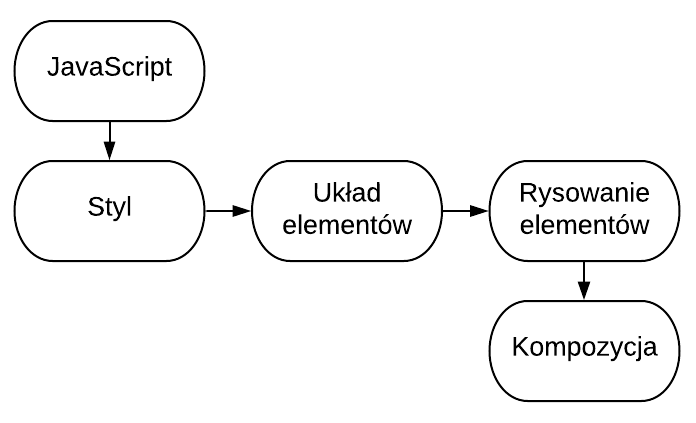
\includegraphics[width=12cm]{rysunek_10.png}
    \caption{Grafika przedstawiająca kolejność faz renderowania w przeglądarce}
    \label{fig:rysunek_10}
\end{figure}

Na początku JavaScript wykonuje zmianę na dokumencie HTML.
Następnie przeglądarka wylicza na podstawie arkusza styli (CSS) pozycję elementów na płótnie przeglądarki.
Następnie znając rozmieszczenie elementów na stronie, przeglądarka wylicza ich wzajemne pozycje oraz rozmiar.
Elementy na stronie mają na siebie wzajemny wpływ na przykład dla dwóch bloków <li>.
W zależności od wysokości pierwszego bloku, drugi blok może zostać wyrenderowany, bądź też nie jeżeli wykracza on poza widoczny obszar rysowania, a także możemy wyliczyć dokładną pozycję na płótnie.
Znając pozycję oraz rozmiary elementów, przechodzimy do fazy malowania.
Pixele zostają malowane na wielu warstwach. W ostatniej fazie kompozycji, warstwy wyświetlone na ekran w konkretnej kolejności (odpowiada za to między innymi atrybut z-index w języku CSS).

Jak widzimy, renderowanie pojedynczej klatki na stronie jest bardzo skomplikowanym procesem, który w idealnym przypadku powinien następować około 60 razy na sekundę (w zależności od  częstotliwości odświeżania ekranu ).
Bardzo istotnym mechanizmem który przeglądarki stosuje w celu optymalizacji ilości pracy jest pomijanie niepotrzebnych fragmentów.
Jeżeli zmianie uległa tylko pewna część strony, na przykład kolor tekstu, możemy pominąć etap wyliczania layoutu strony.
Jeżeli nastąpi zmiana stanu, w której nie wystąpiła zmiana ani layoutu ani nie występuje potrzeba ponownego malowania, przeglądarka użyje poprzedniego zestawu gotowych warstw.
Zrozumienie tego mechanizmu jest istotnym czynnikiem na którym oparłem konstrukcję testów wydajnościowych.

Wracając do samej konstrukcji testu. Znając już mechanizm omijania czynności podczas renderowania obrazu w przeglądarce możemy przedstawić problem renderowania list.
Załóżmy, że mamy listę 20 wyrenderowanych elementów na stronie. Do listy możemy dopisać nowe wartości albo na początku albo na końcu.
W pierwszym kroku, dopisuję jeden nowy element do listy, na końcu co przedstawiono na rysunku \ref{fig:rysunek_11}. Każdy element na liście ma przypisany indeks.
Dopisując nowy element do listy, w optymalnym przypadku, powinienem wyrenderować tylko jeden nowy element i dokładnie tak się stanie. Co stanie się, gdy dopiszę nowy element na początku listy? Otóż wszystkie indeksy zostaną przesunięte o 1.
React wykryje zmianę jednego elementu na liście, i przeglądarka wyrenderuje tylko jeden nowy element . Widzimy także, że znaczna część fazy layoutu będzie taka sama, gdyż na ekranie zmieni się tylko jeden widoczny element.

\begin{figure}[!ht]
    \centering
    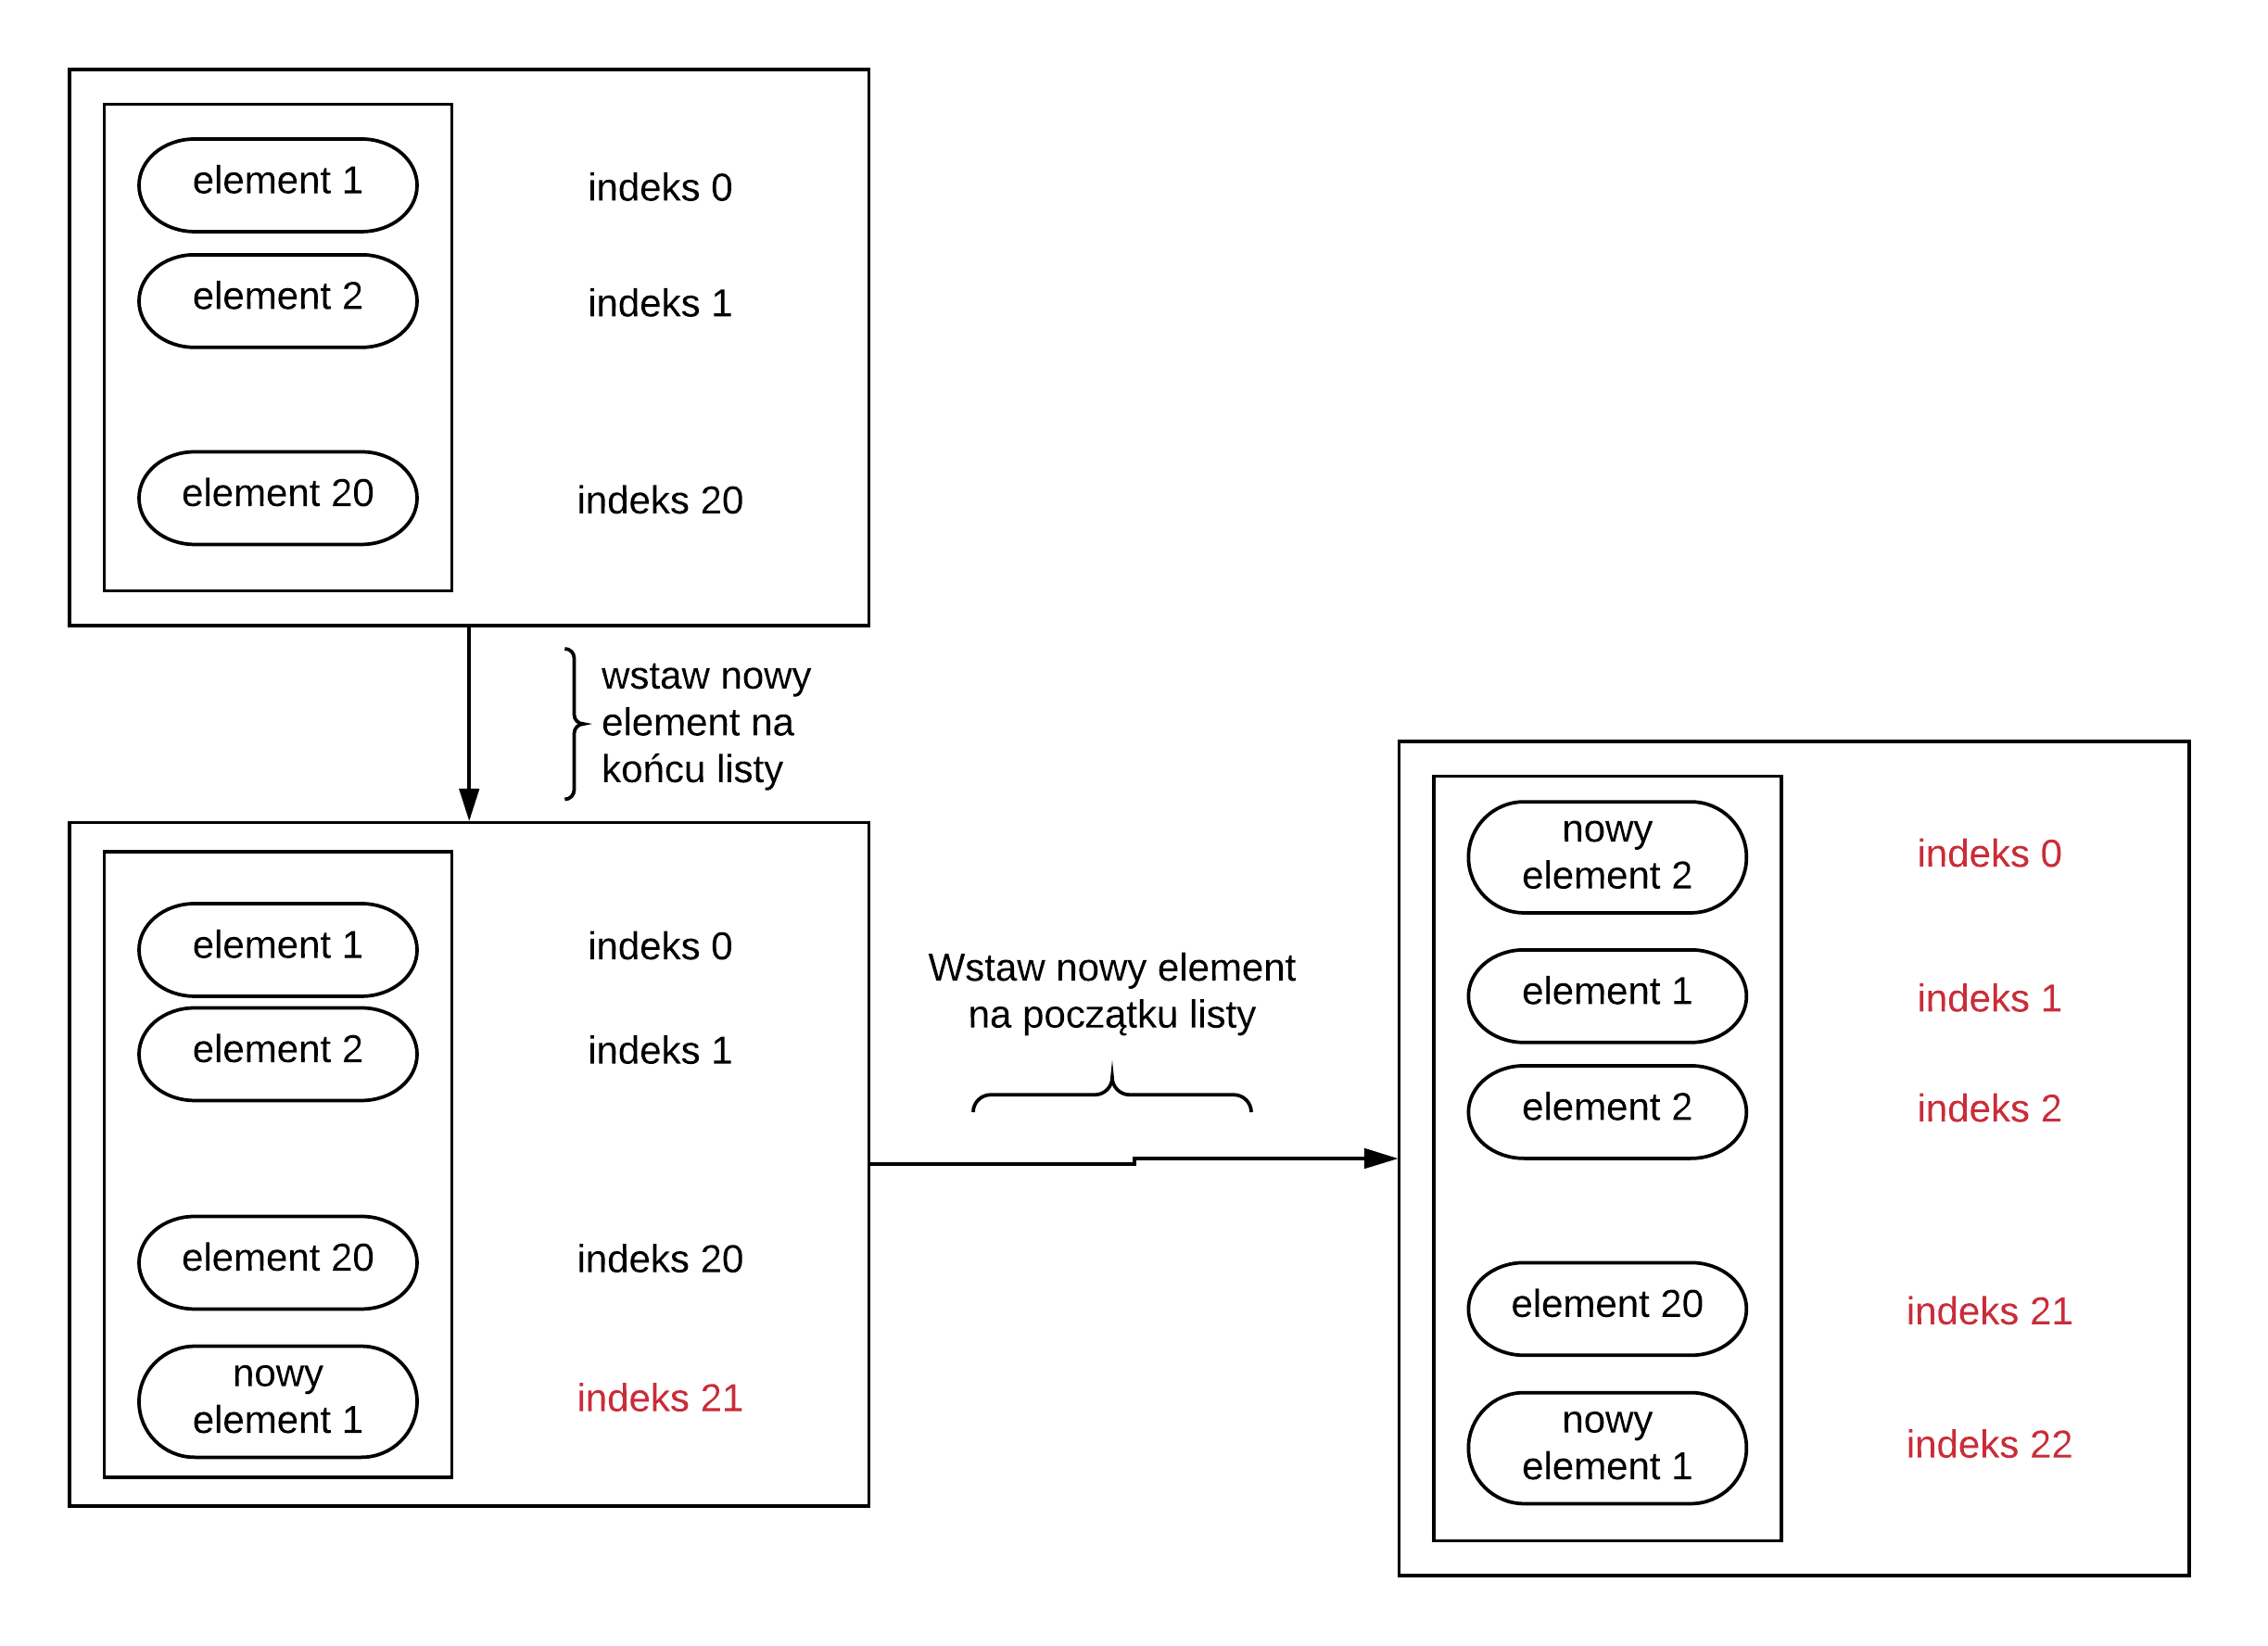
\includegraphics[width=12cm]{rysunek_11.png}
    \caption{Ilustracja przedstawiająca problem dopisywania elementu na koniec listy}
    \label{fig:rysunek_11}
\end{figure}

Co stanie się w przypadku dopisania jednego nowego elementu na początku listy? Problem ten zaprezentowano na rysunku 12. Każdy indeks przypisany do elementu zostanie przesunięty o jeden.
Z racji tej, React ponownie wyrenderuje każdy element (gdyż uzna, iż jest to nowy element). Spowoduje to zmianę kodu HTML która zmusi przeglądarkę do pełnego prze renderowania wszystkich warstw oraz wyliczenia całego layoutu na nowo.
Oczywiście w skali 20 elementów które nie posiadają skomplikowanej struktury HTML i stylowania CSS nie powinno to robić problemu.
Jednak w dobie nowoczesnych aplikacji, listy (np lista filmów netflixa) posiadają masę małych elementów przez co lista nawet 50 elementów może spowodować zauważalne opóźnienia podczas użytkowania aplikacji.

W jaki sposób możemy poradzić sobie z tym problemem? Istnieją dwa sposoby dzięki którym React obiecuje znacznie wyższą wydajność w porównaniu do czystego kodu JavaScript.
Pierwszym z nich jest unikalny indeks elementu \cite{react-lists}. Zamiast stosować klucza równego indeksowi elementu, musimy podać klucz który jest unikalny w ramach elementu.
Przykładowo dla każdego elementu stworzymy parę (klucz, hasz). W tym momencie, jeżeli dodamy nowy element na początku listy, React spojrzy na listę kluczy, i zobaczy, że nie zmieniły się one, a dodano tylko jeden nowy element.
Zamiast 22 renredowań, otrzymamy tylko jedno.

\begin{figure}[!ht]
    \centering
    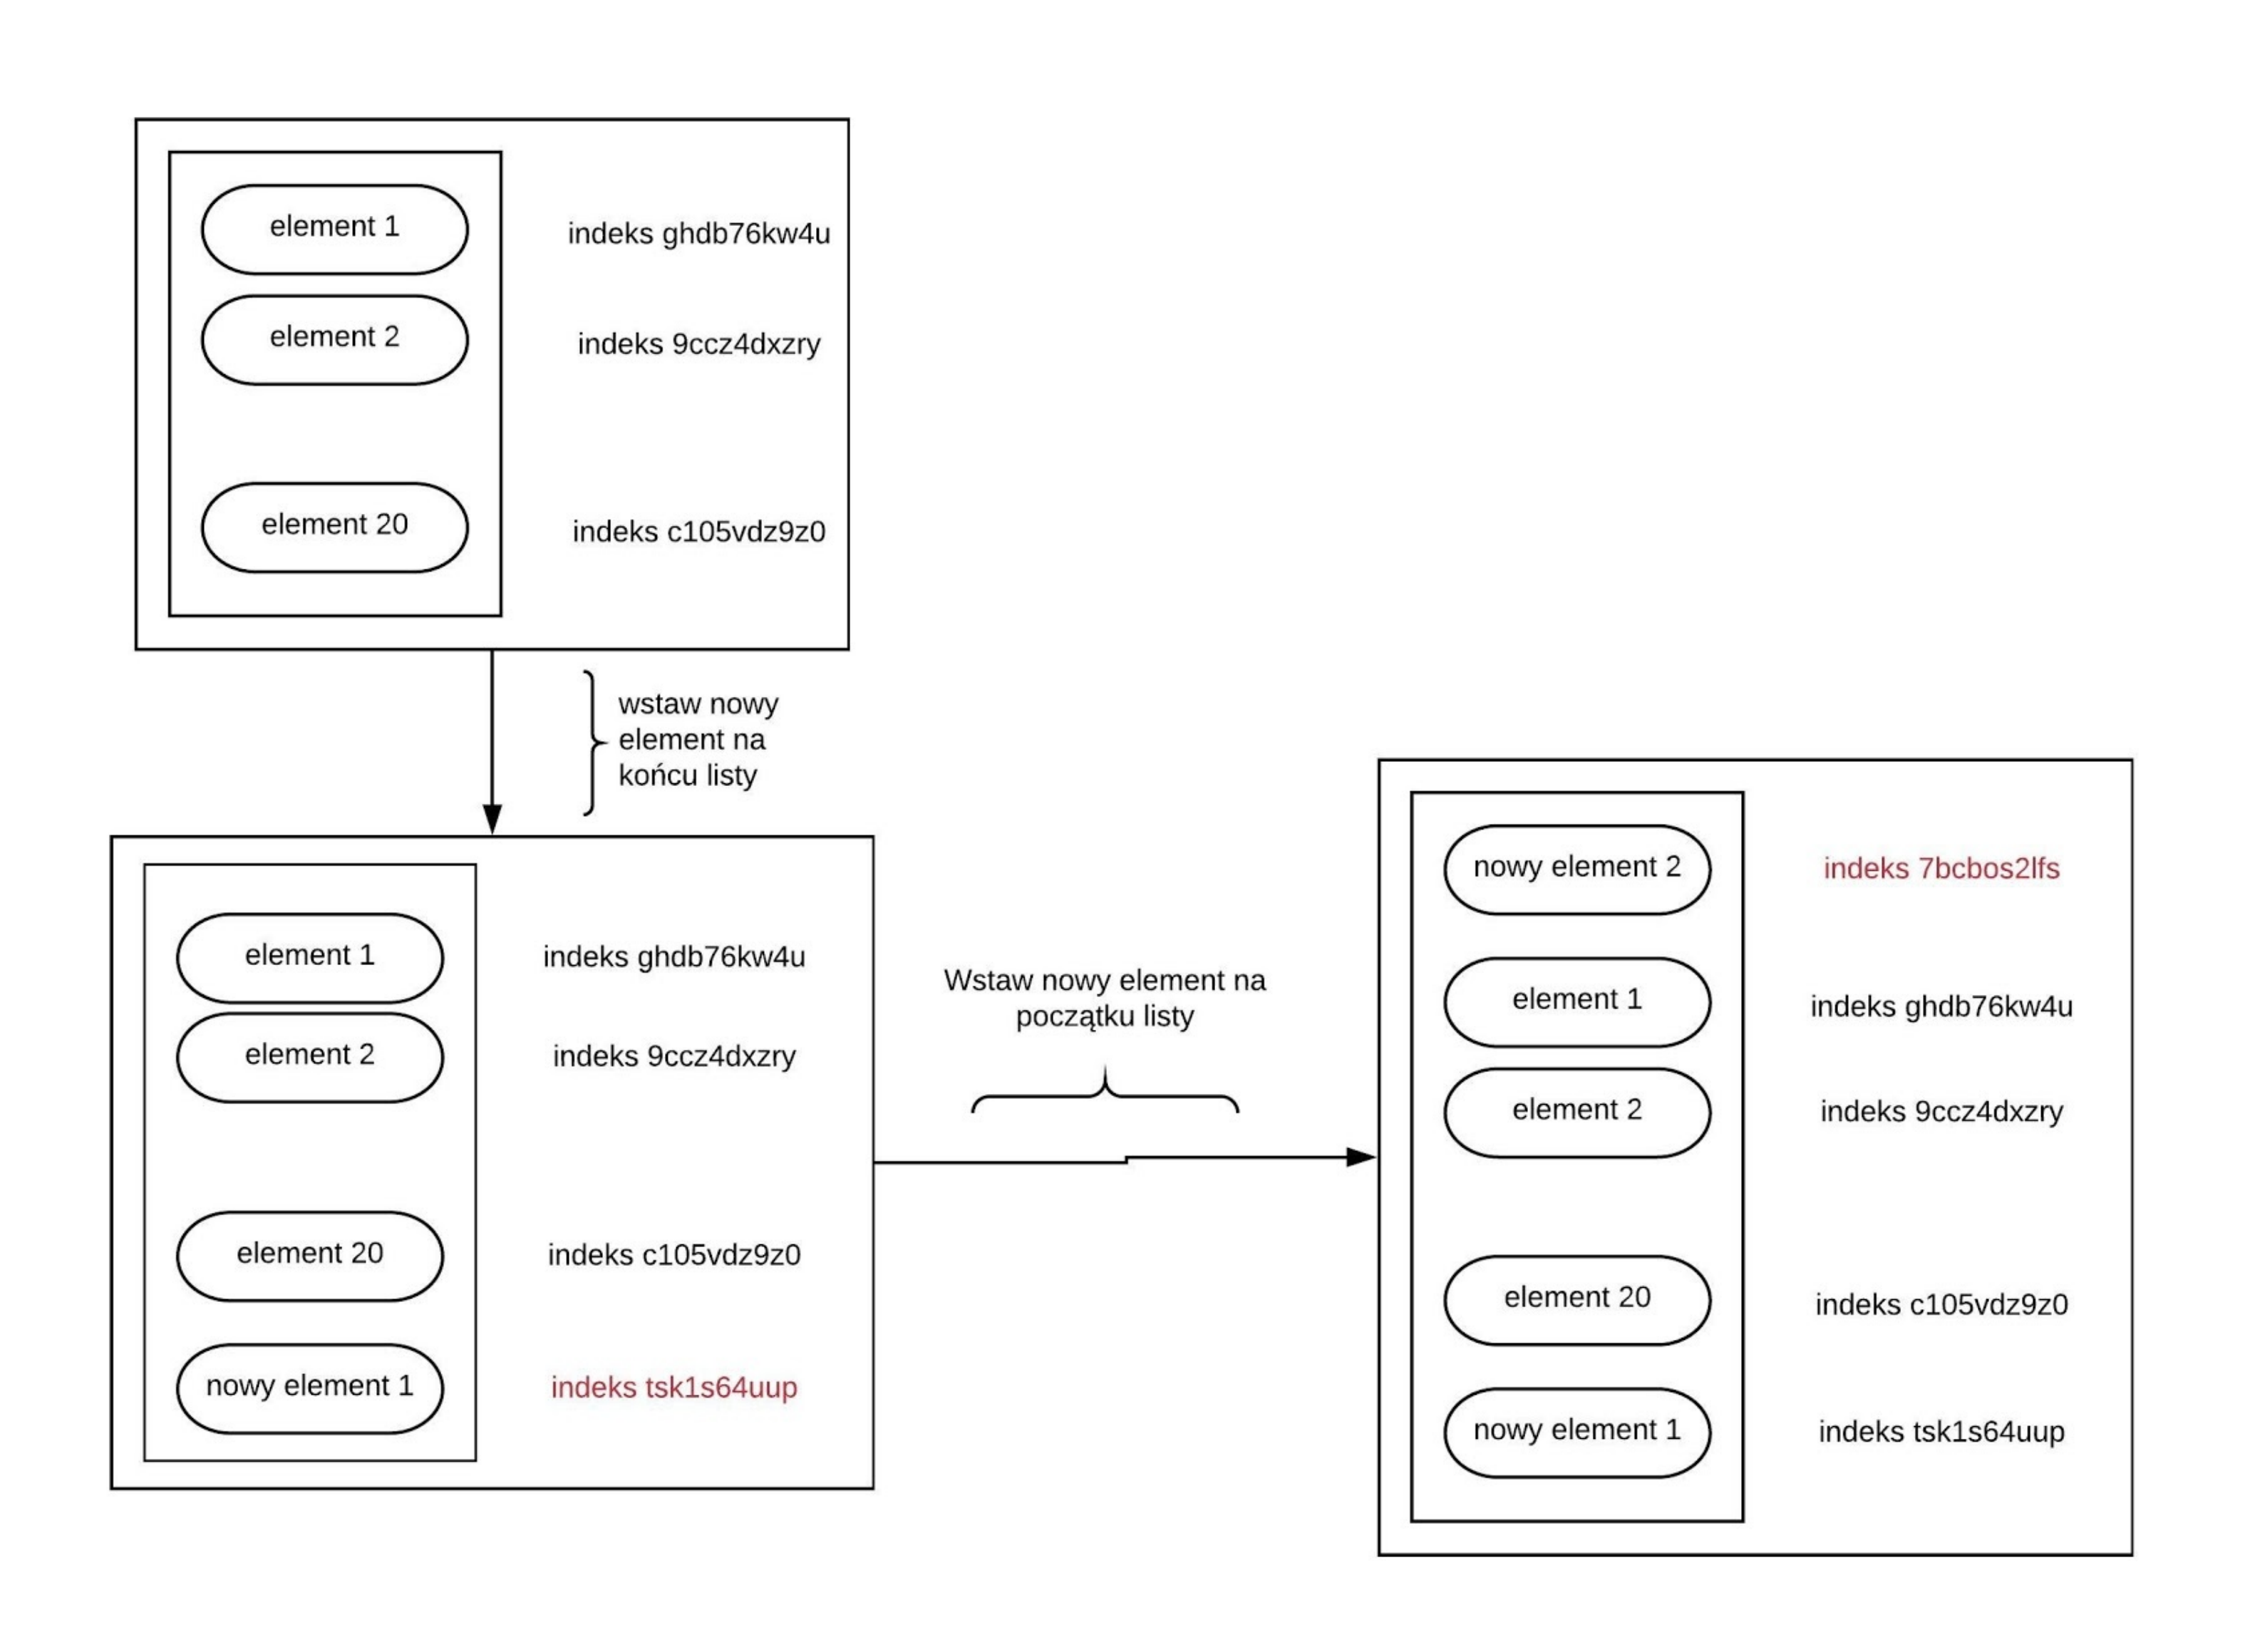
\includegraphics[width=12cm]{rysunek_12.png}
    \caption{Ilustracja przedstawiająca problem dopisywania elementów na początek listy}
    \label{fig:rysunek_12}
\end{figure}

Drugim sposobem poradzenia sobie z minimalizacją ilości renderowania jest koncepcja wirtualnego modelu DOM \cite{virtualdom}.
Jest to mechanizm, który tworzy reprezentację interfejsu użytkownika w pamięci i synchronizuje ją z modelem DOM przeglądarki. Proces ten nazywa się rekoncyliacją \cite{reconcilation}.
Pozwala to na wyrenderowanie tylko tych elementów, które różnią się między reprezentacją w pamięci a reprezentacją faktyczną drzewa DOM.

Znając już konkretny problem, z którym aplikacje SPA muszą się mierzyć, postanowiono zaprojektować szereg akcji manipulujących listą elementów oraz zbadać, ile czasu zajmie konkretnego frameworkowi wykonanie takiej czynności.

\subsection{Budowa aplikacji}

Każda aplikacja będzie składać się z szeregu przycisków. W wewnętrznym stanie aplikacji, będziemy trzymać listę wartości do wyrenderowania. Wartości które będziemy renderować będą stringiem o długości 10 znaków. Proces zmiany aplikacji prezentuję na poniższym rysunku.
\begin{figure}[!ht]
    \centering
    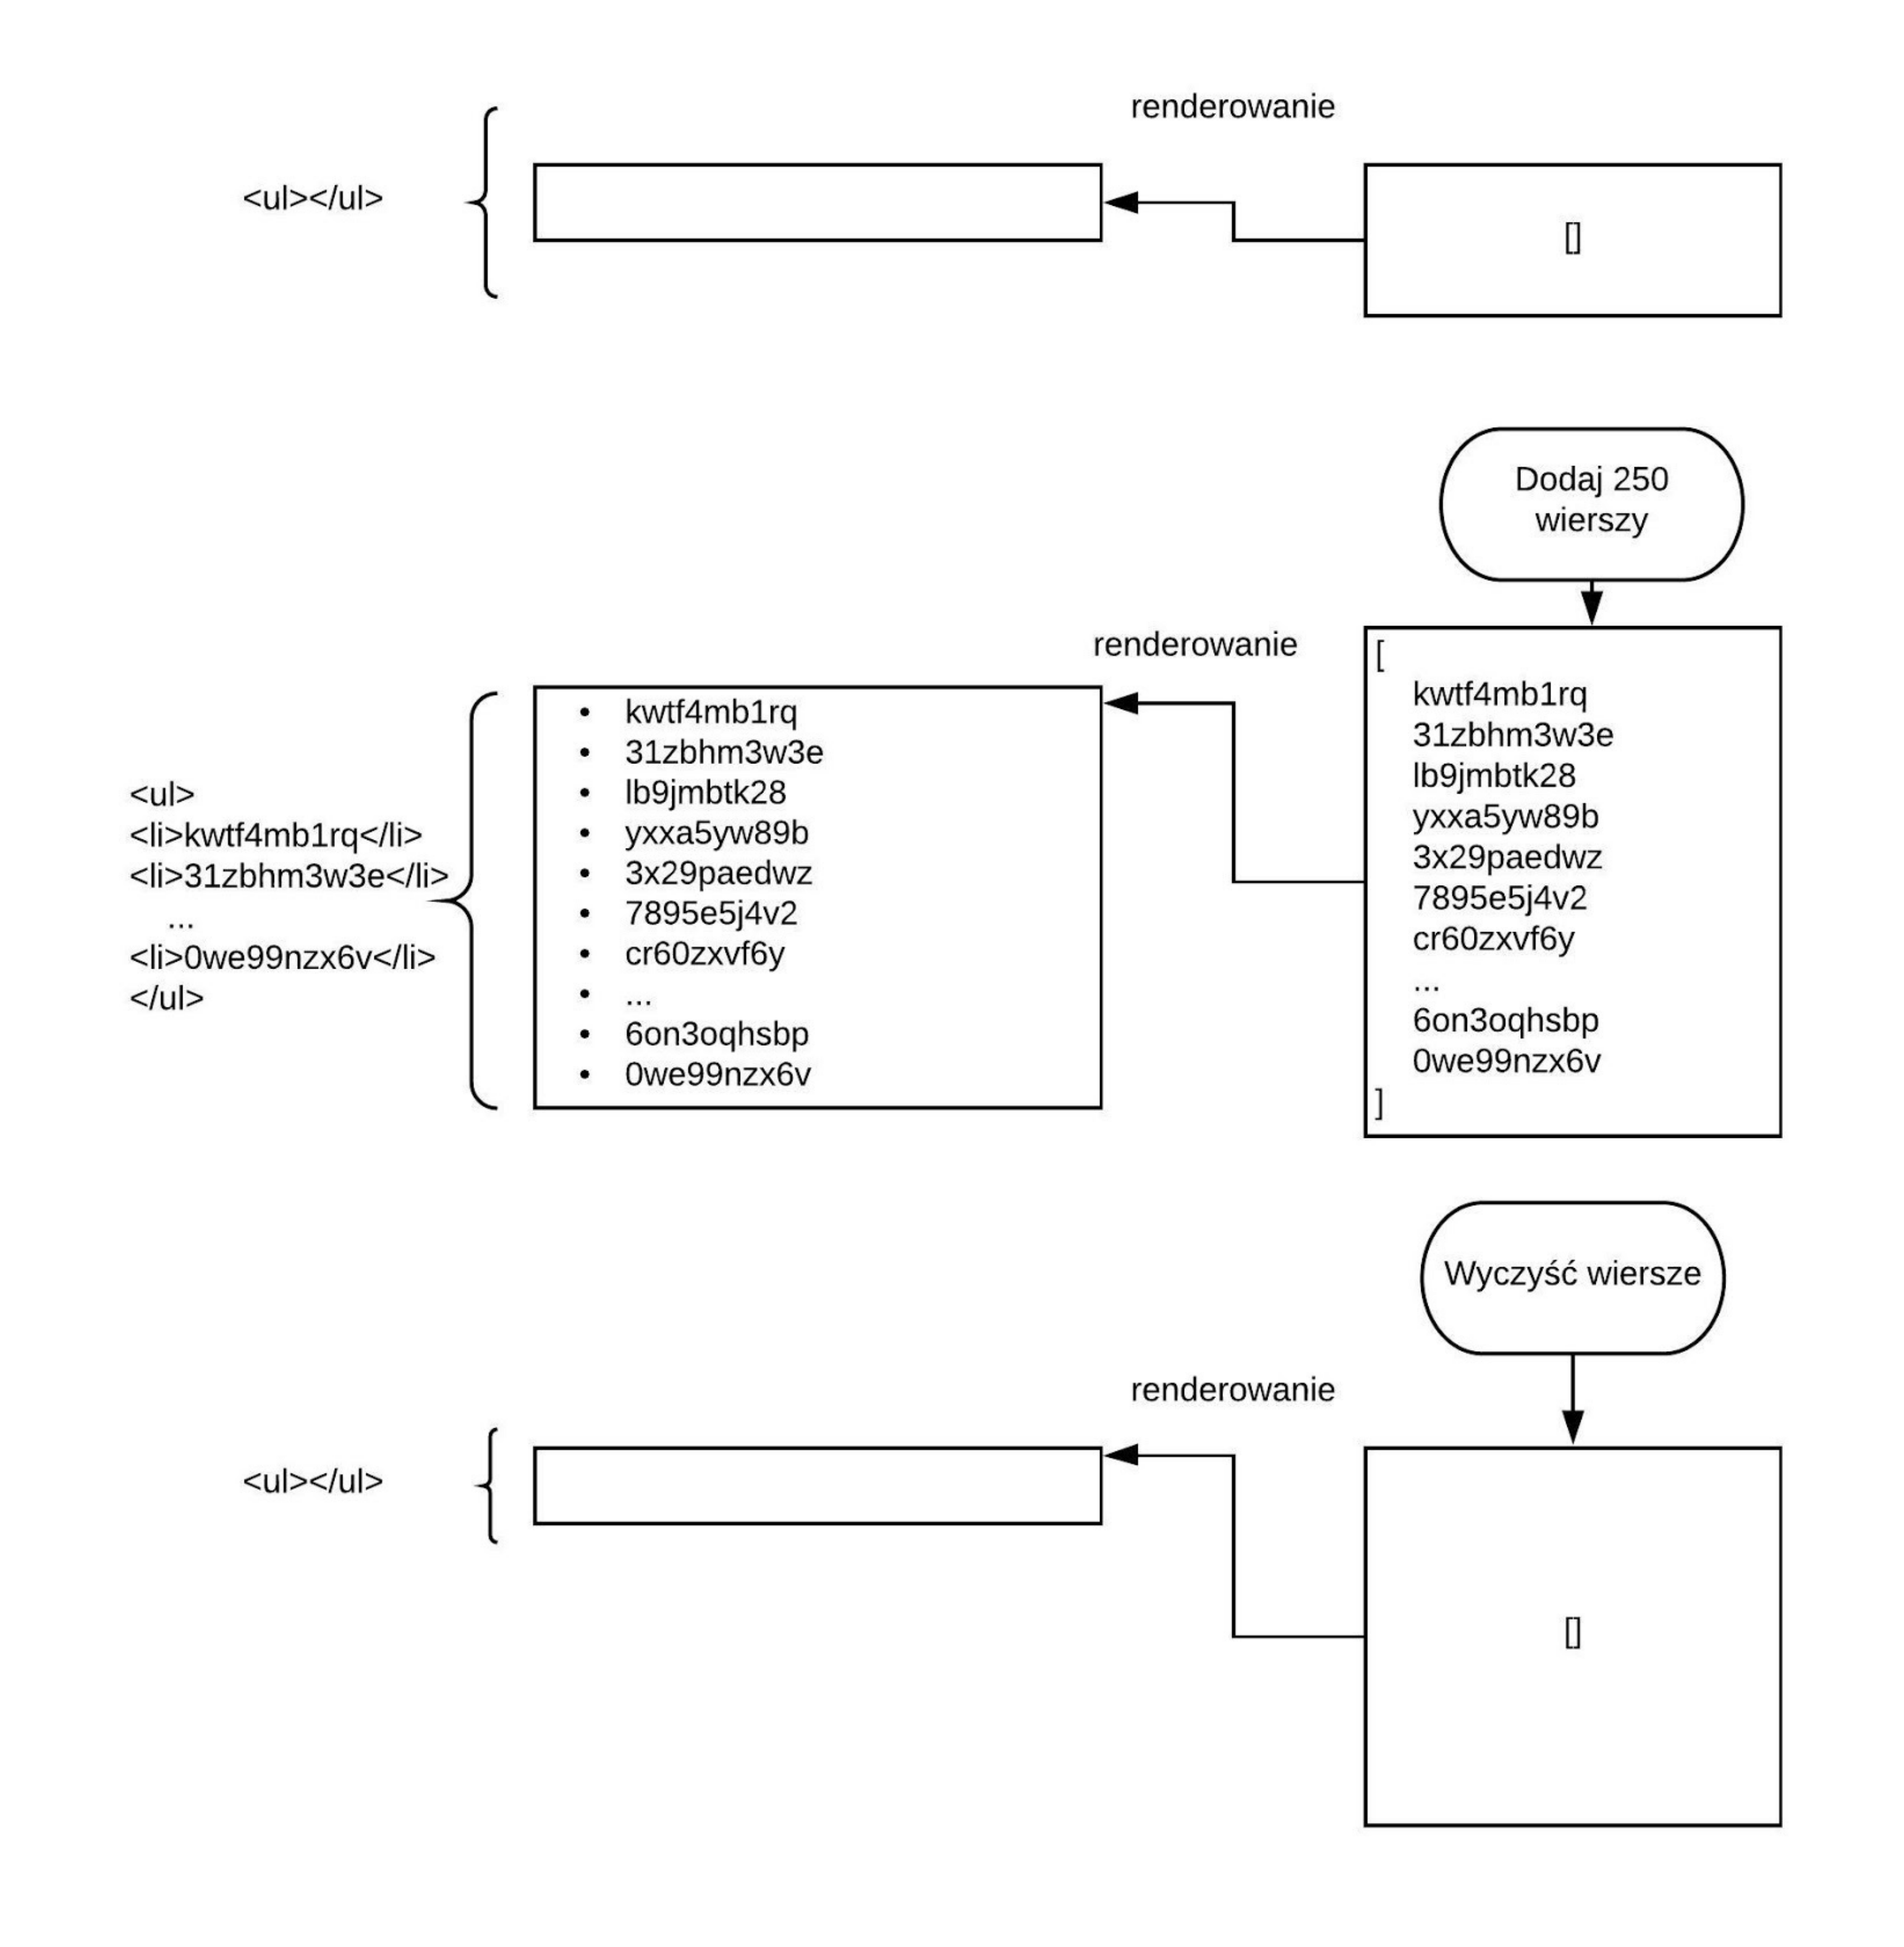
\includegraphics[width=12cm]{rysunek_13.png}
    \caption{Ilustracja mechanizmu przebiegu badania}
    \label{fig:rysunek_13}
\end{figure}

Na początku stan wewnętrzny aplikacji będzie pustą tablicą. Spowoduje to wyrenderowanie stanu minimalnego, czyli bloku <ul>.
Akcja naciśnięcia przycisku spowoduje wygenerowanie 250 wpisów zawierających wylosowane alfanumeryczne wartości. Wartości te muszą być, w miarę możliwości unikatowe.
Zmiana stanu z kolei spowoduje ponowne wyrenderowanie komponentu wyświetlającego listę. Kolejne akcje będą działać w myśl tej samej zasady.

Na rysunku poniżej przedstawiam listę akcji jakie aplikacja musi implementować:

\begin{figure}[!ht]
    \centering
    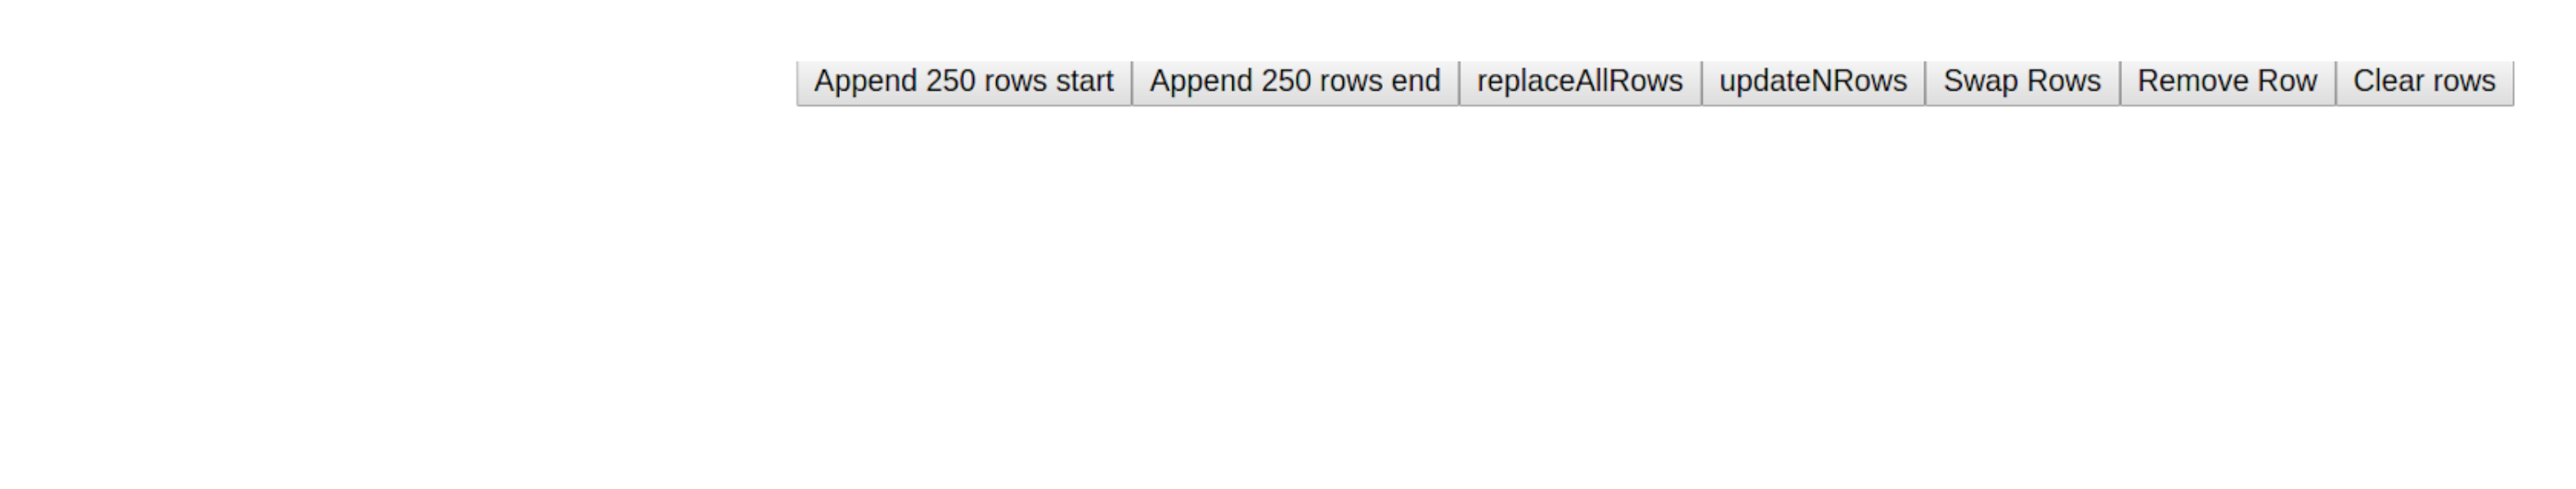
\includegraphics[width=12cm]{rysunek_14.png}
    \caption{Grafika przedstawiająca zaimplementowane przyciski w aplikacji}
    \label{fig:rysunek_14}
\end{figure}

\begin{itemize}
    \item \emph{Append 250 rows start} - dodaj 250 wierszy na początku listy.
    \item \emph{Append 250 rows end} - dodaj 250 wierszy na końcu listy.
    \item \emph{Replace all rows} - wygeneruj na nowo pełną listę wartości
    \item \emph{Update N rows} - wybierz losowo 250 wierszy i zaktualizuj ich wartości
    \item \emph{Swap rows} - zamień miejscami 2 wiersze
    \item \emph{Remove row} - usuń jeden wiesz
    \item \emph{Clear rows} - usuń wszystkie wiersze
\end{itemize}

Na początku części praktycznej wprowadzono definicję akcji aplikacji. Widzimy tutaj, iż samo przyciśnięcie przycisku dodania aplikacji nie jest wystarczające, gdyż przed wyrenderowaniem listy musimy wygenerować listę wpisów.
Renderowanie aplikacji także jest nie deterministyczne, i wpływ na nie ma szereg czynników niezależnych od przeglądarki.
Spowoduje to znaczne różnice w wynikach pomiaru czasu akcji aplikacji, z tego też powodu istotnym jest upewnienie się, iż kolejne iteracje badania są od siebie możliwie niezależne.

Ostatnim elementem składającym się na aplikację jest jej infrastruktura. Każda aplikacja tworzona jest w całkowicie inny sposób, dlatego istotnym jest, aby ujednolicić proces budowania i pakowania plików wynikowych.
Z racji tego, każda aplikacja musi posiadać w sobie plik Makefile \cite{gnu-makefile} z dwoma możliwymi celami:

\begin{itemize}
    \item install
    \item Production
\end{itemize}

Cel \emph{install} jak sama nazwa wskazuje, przygotuje folder \emph{node\_modules} zawierający pobrane biblioteki z platformy NPM \cite{npm}
Drugi cel \emph{production} zajmie się procesem pakowania aplikacji i optymalizacji kodu w celach produkcyjnych \cite{react-perf}.

\subsection{Przygotowanie aplikacji do badania}
\subsection{Konteneryzacja aplikacji}
\subsection{Moduł badania}
\subsection{Moduł analizy}

\section{Analiza wyników}
\subsection{Czas załadowania aplikacji}
\subsection{Dodanie 1000 wierszy na początku listy}
\subsection{Dodanie 1000 wierszy na końcu listy}
\subsection{Zamiana wszystkich wierszy na liście}
\subsection{Aktualizacja 500 wierszy}
\subsection{Zamiana miejscami dwóch wierszy}
\subsection{Usunięcie pojedynczego wiersza}
\subsection{Usunięcie wszystkich wierszy}


% \begin{figure}[!ht]
%     \centering
%     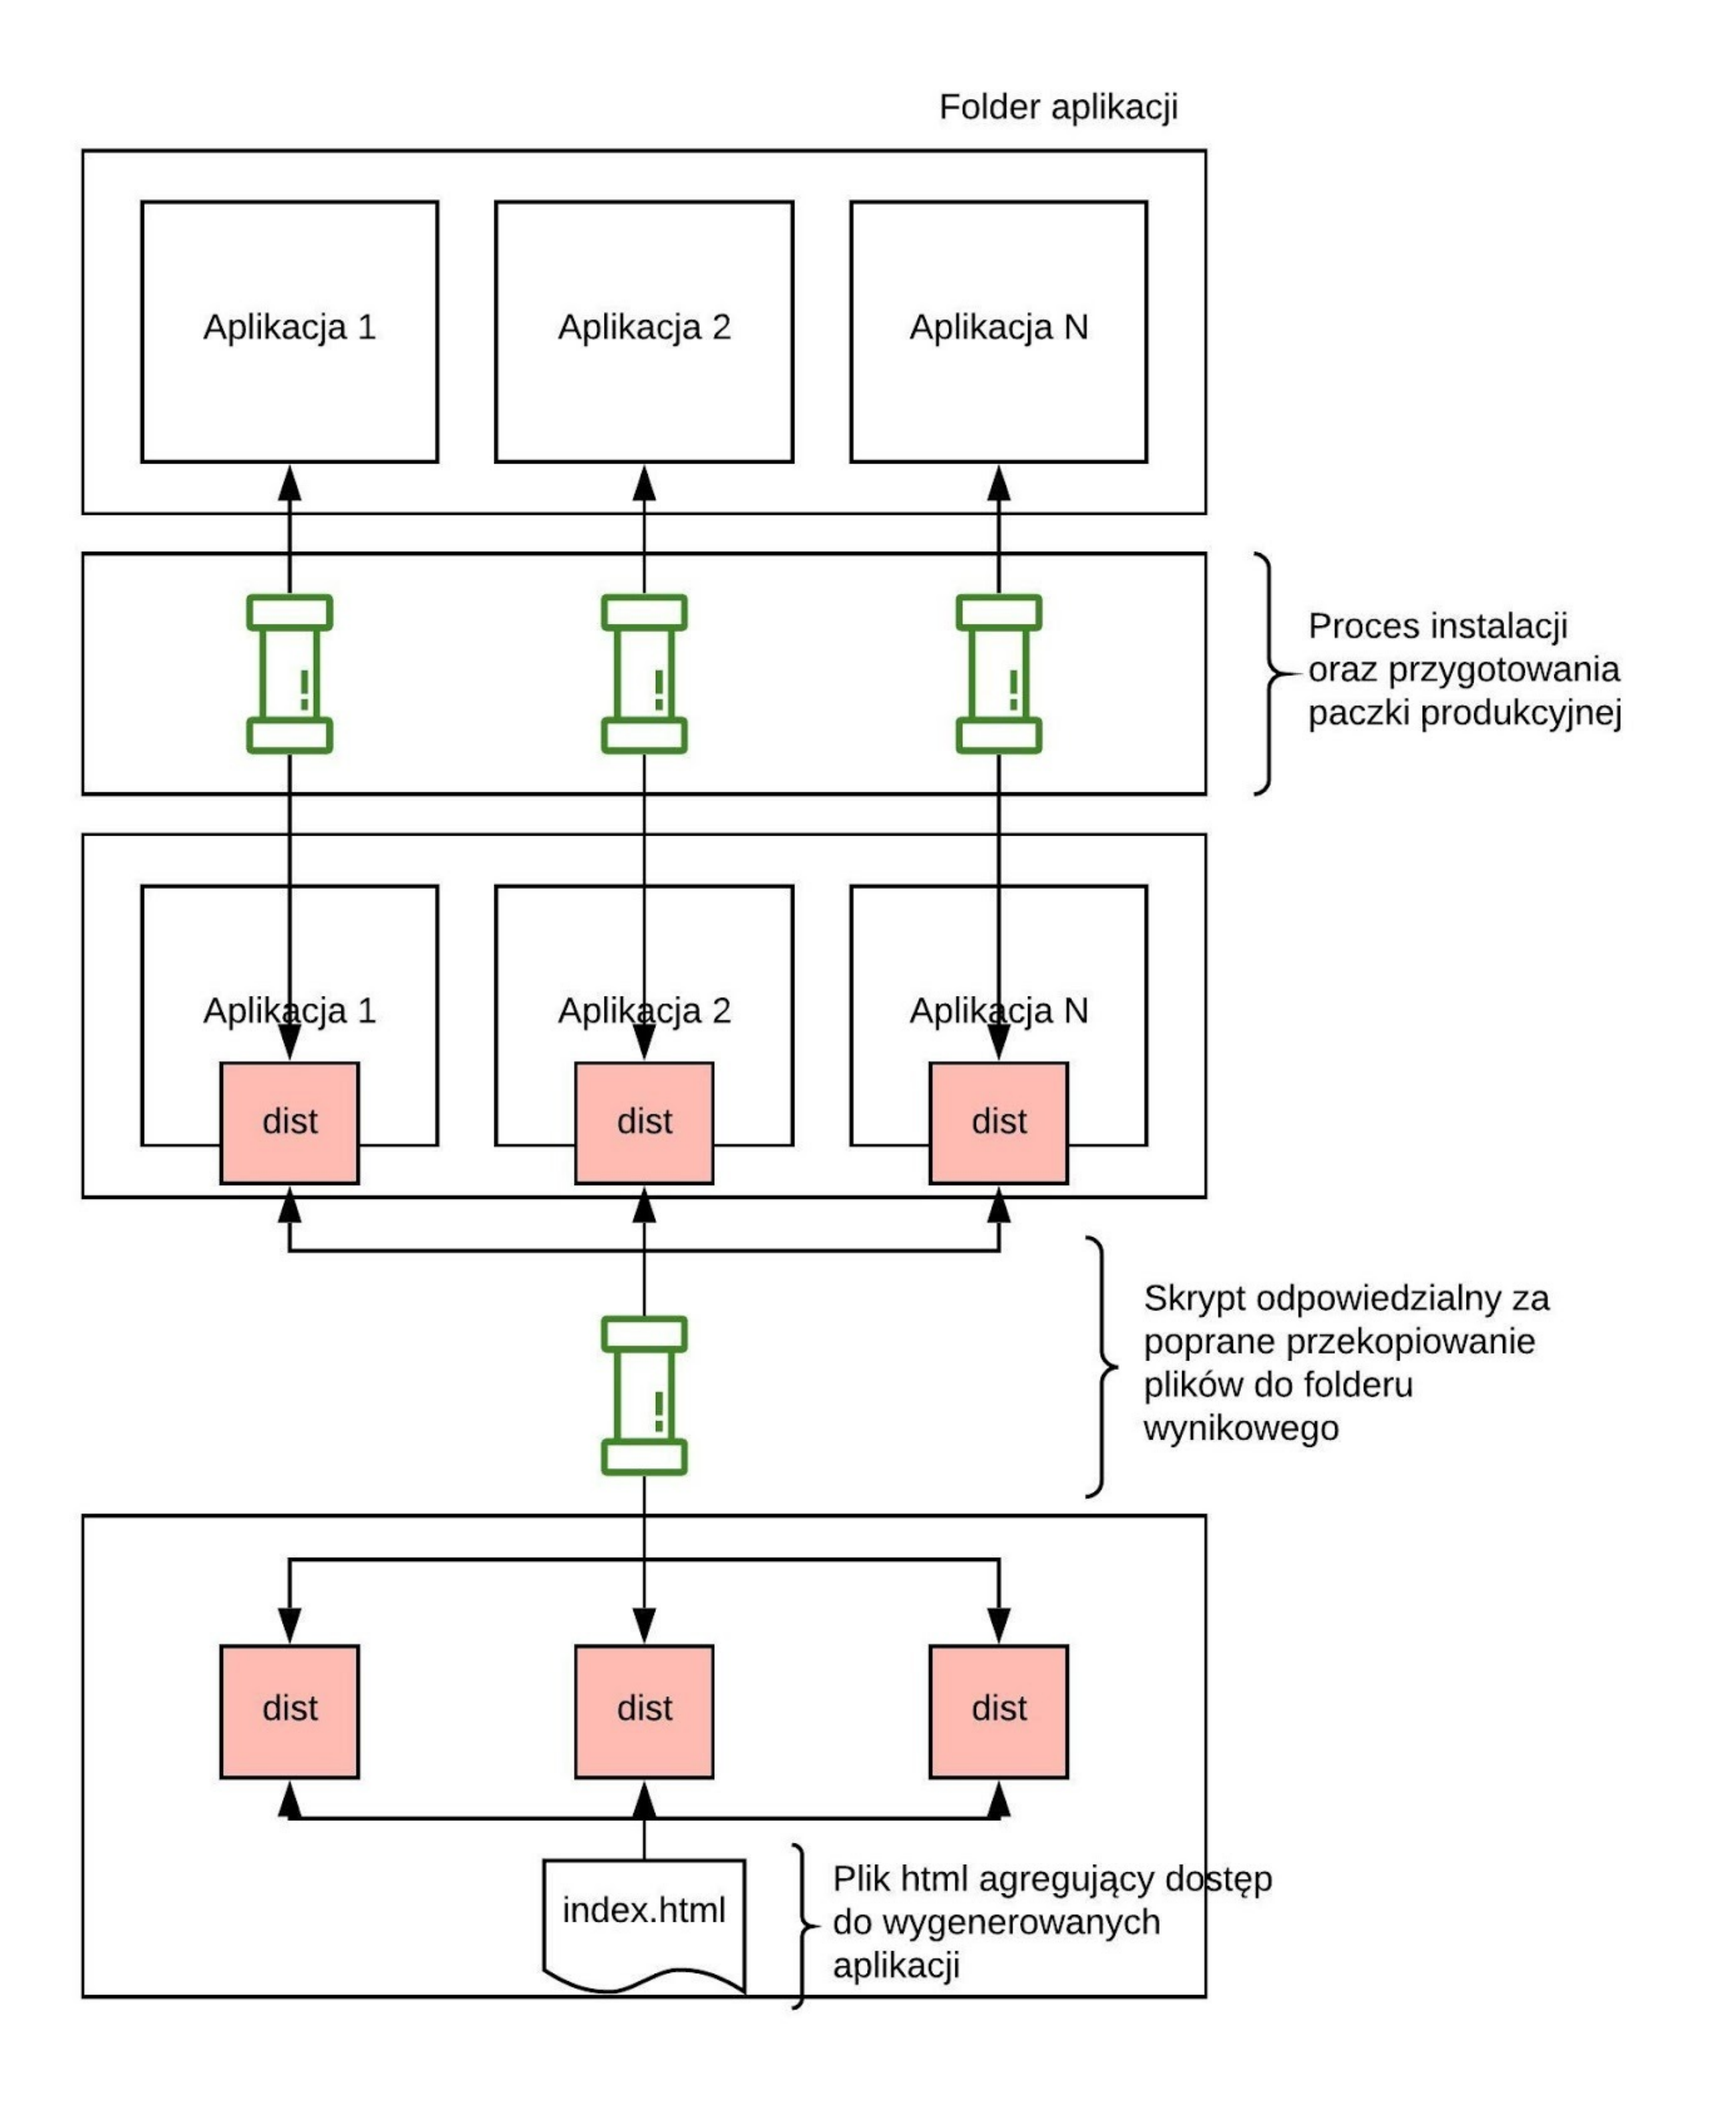
\includegraphics[width=12cm]{rysunek_15.png}
%     \caption{Ilustracja procesu przygotowania aplikacji do konteneryzacji}
%     \label{fig:rysunek_15}
% \end{figure}

% \begin{figure}[!ht]
%     \centering
%     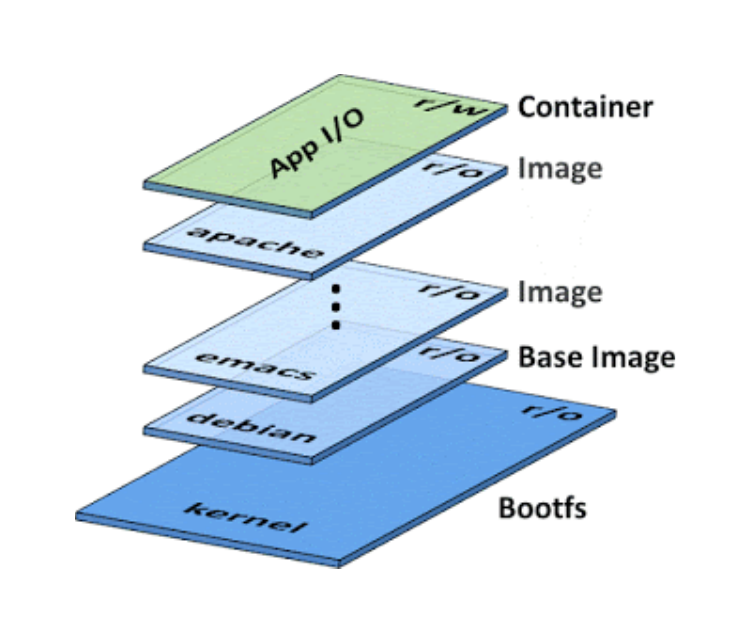
\includegraphics[width=12cm]{rysunek_16.png}
%     \caption{Ilustracja przedstawiająca warstwy składające się na  przykładowy obraz dockera}
%     \label{fig:rysunek_16}
% \end{figure}

% \begin{figure}[!ht]
%     \centering
%     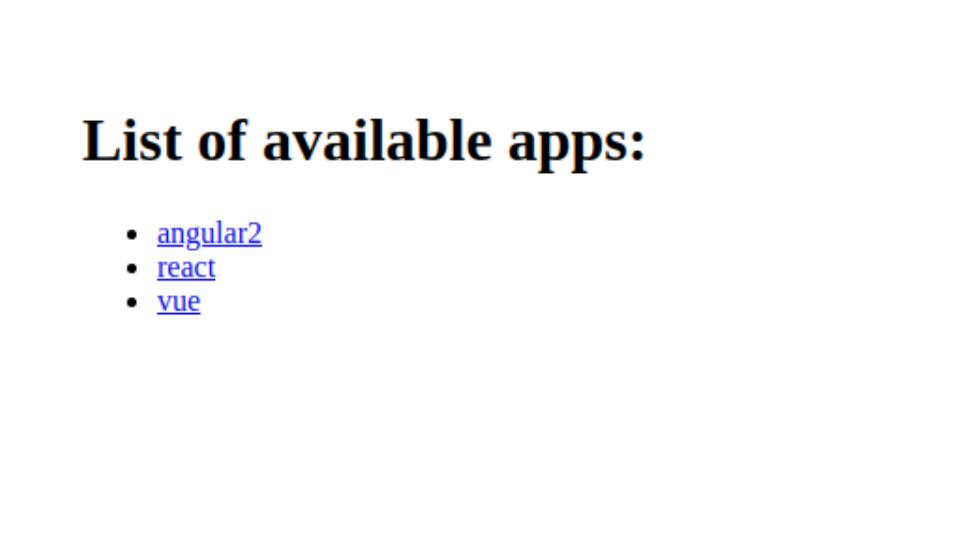
\includegraphics[width=12cm]{rysunek_17.png}
%     \caption{Grafika przedstawiająca plik index.html wraz z dostępnymi aplikacjami do badania}
%     \label{fig:rysunek_17}
% \end{figure}

% \begin{figure}[!ht]
%     \centering
%     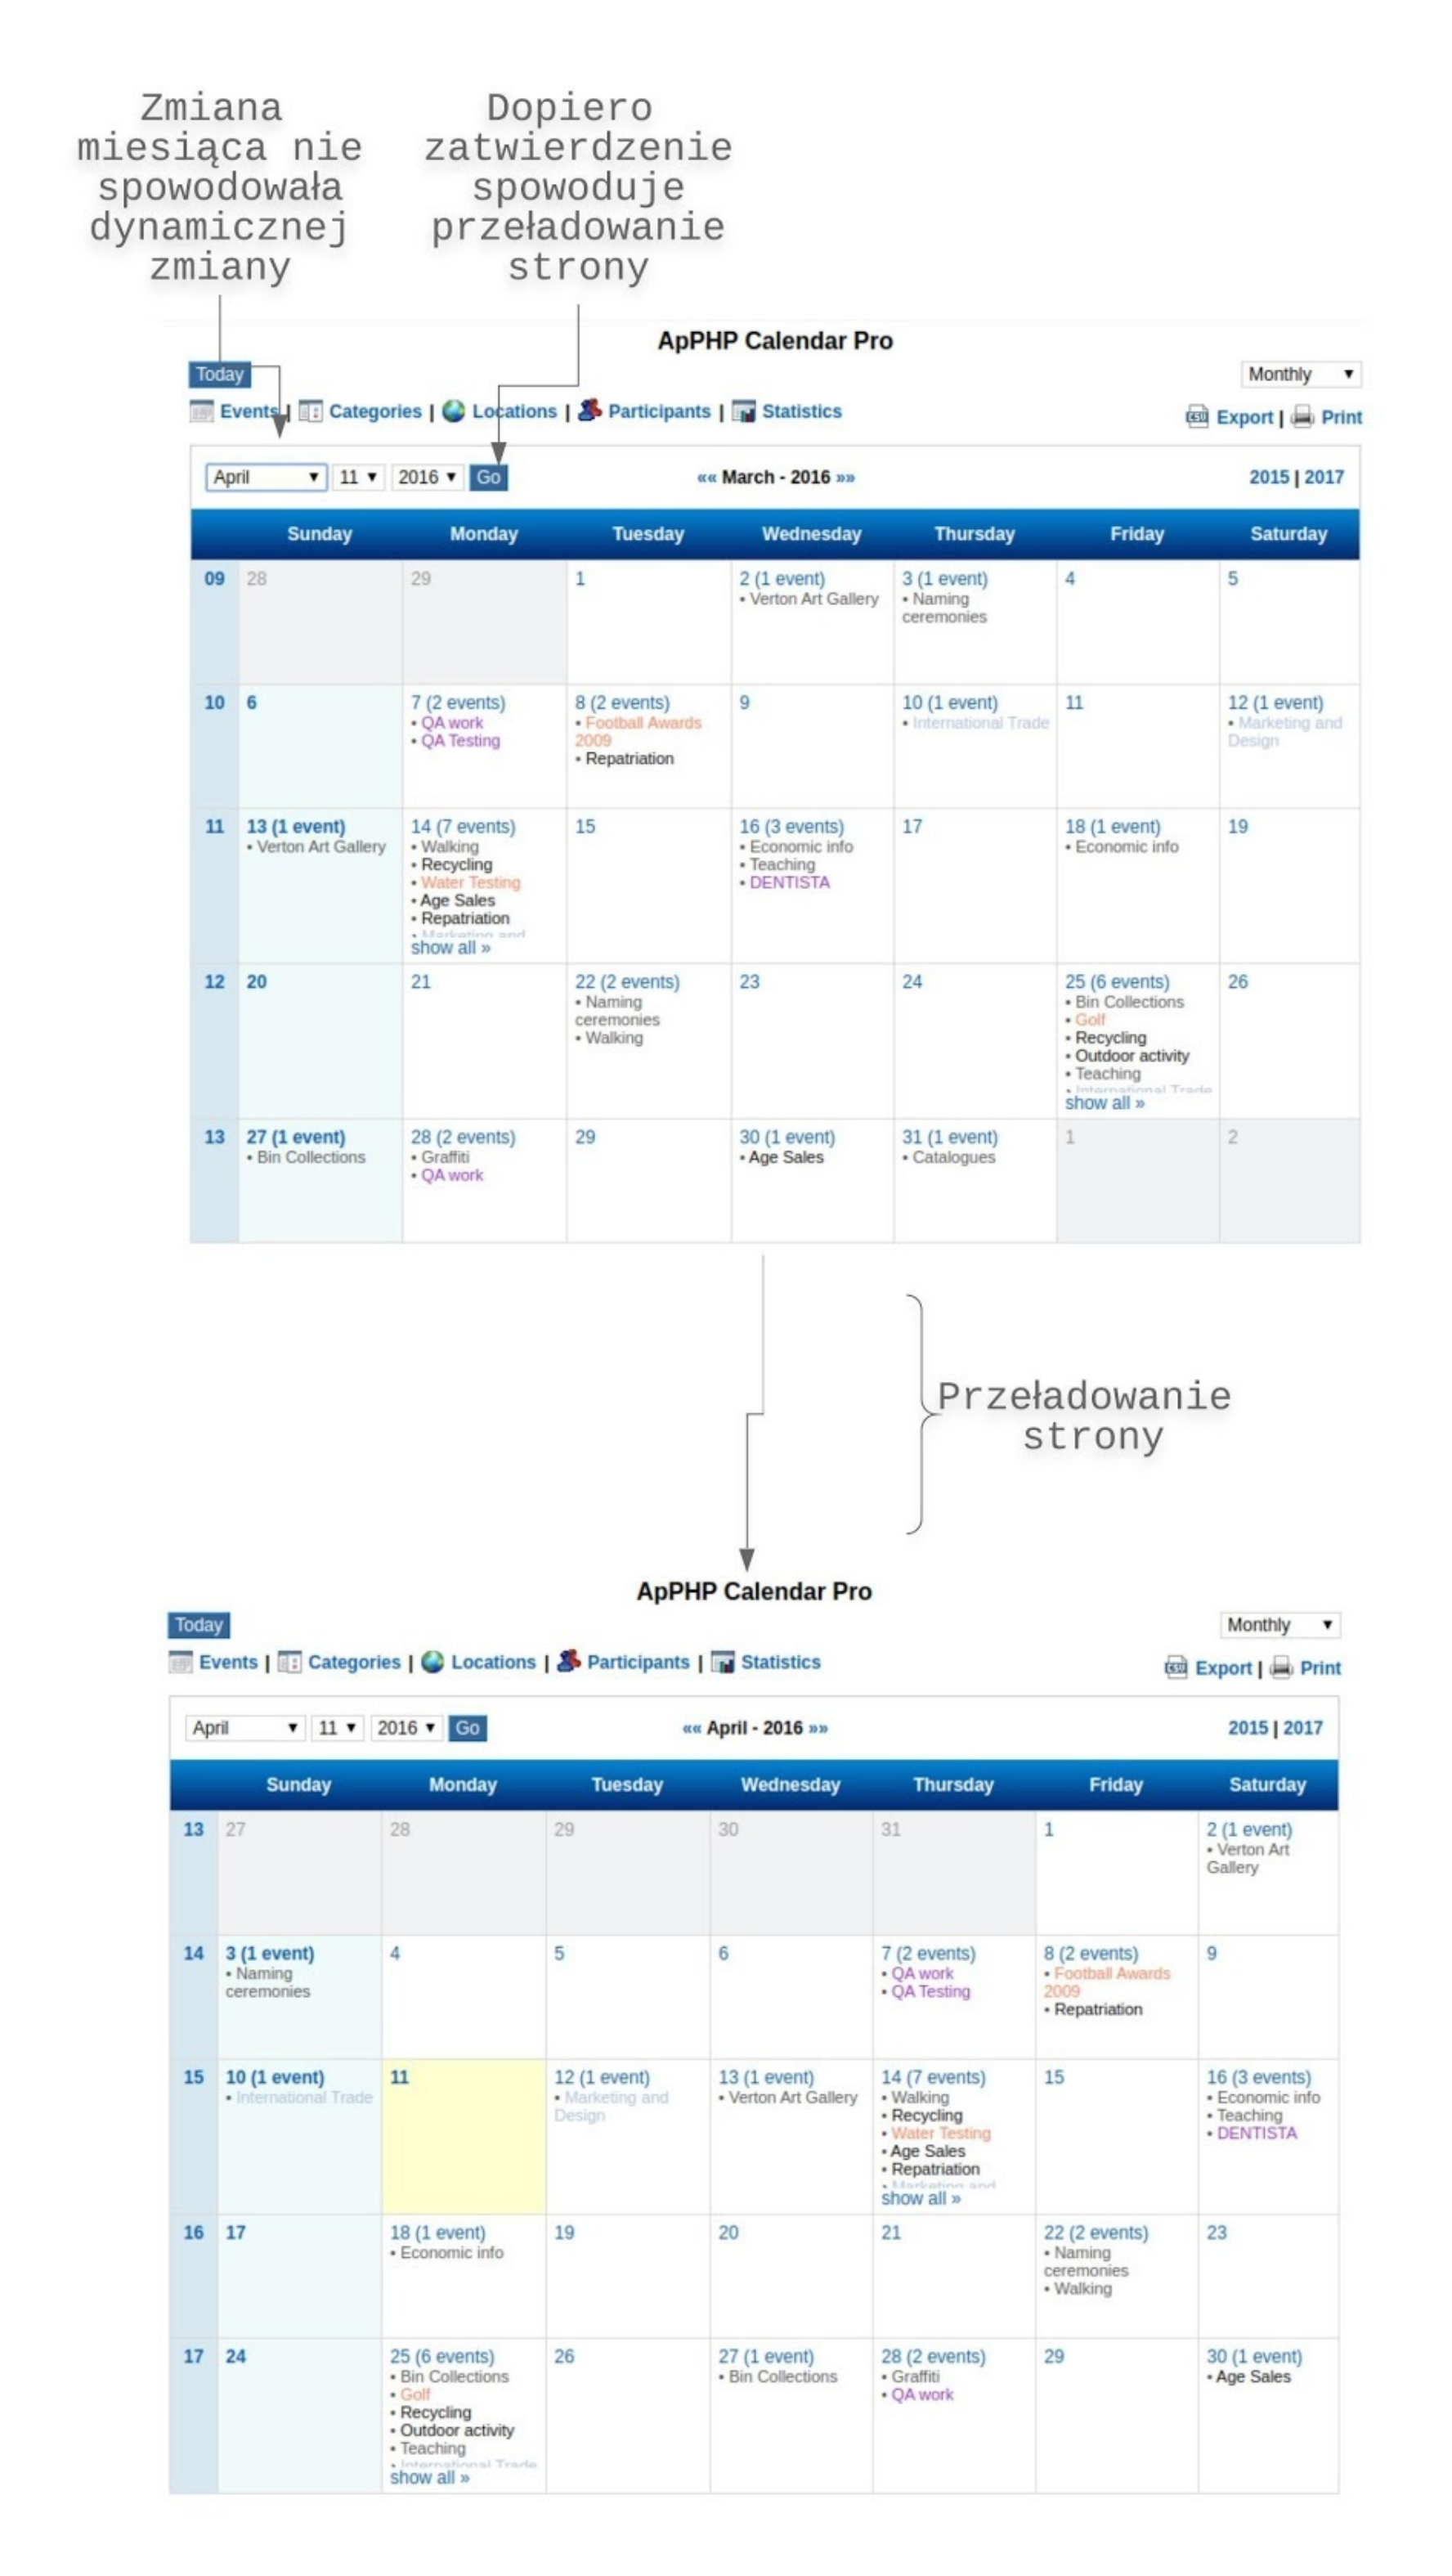
\includegraphics[width=12cm]{rysunek_18.png}
%     \caption{Ilustracja mechanizmu działania strony statycznej na przykładzie aplikacji kalendarza przy użyciu języka PHP}
%     \label{fig:rysunek_18}
% \end{figure}

% \begin{figure}[!ht]
%     \centering
%     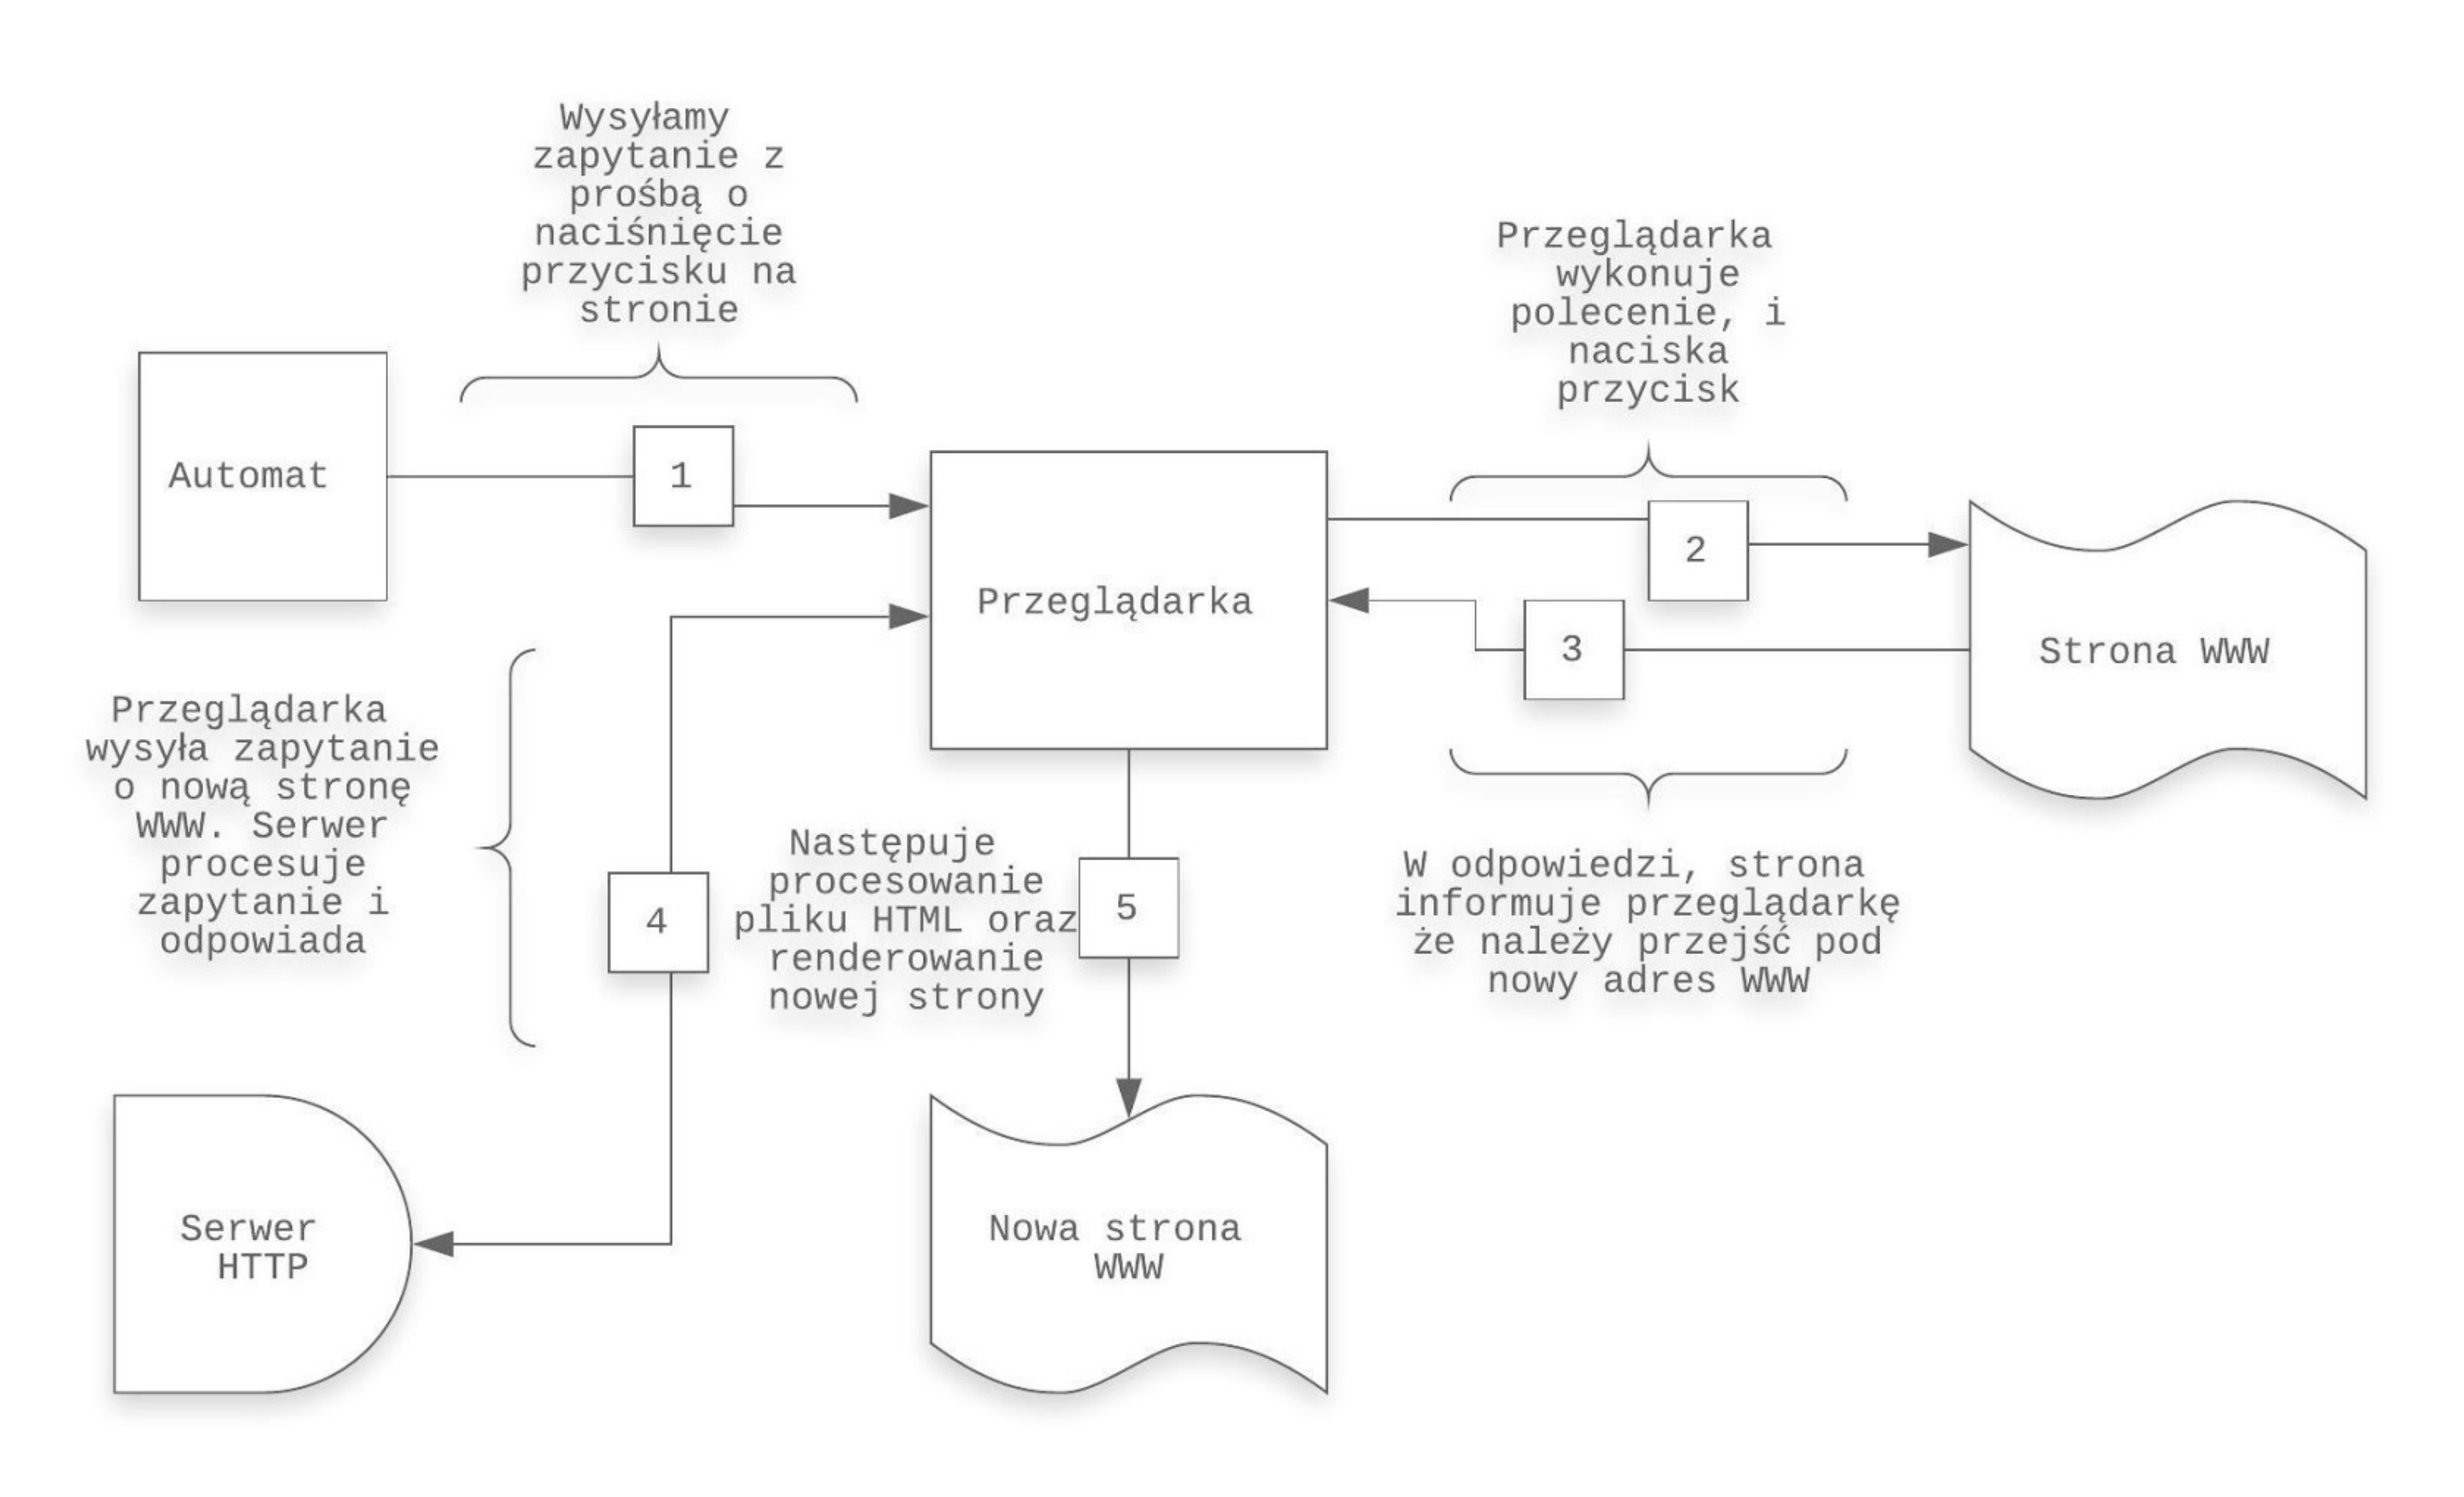
\includegraphics[width=12cm]{rysunek_19.png}
%     \caption{Grafika przedstawiająca proces przeładowania strony statycznej}
%     \label{fig:rysunek_19}
% \end{figure}

% \begin{figure}[!ht]
%     \centering
%     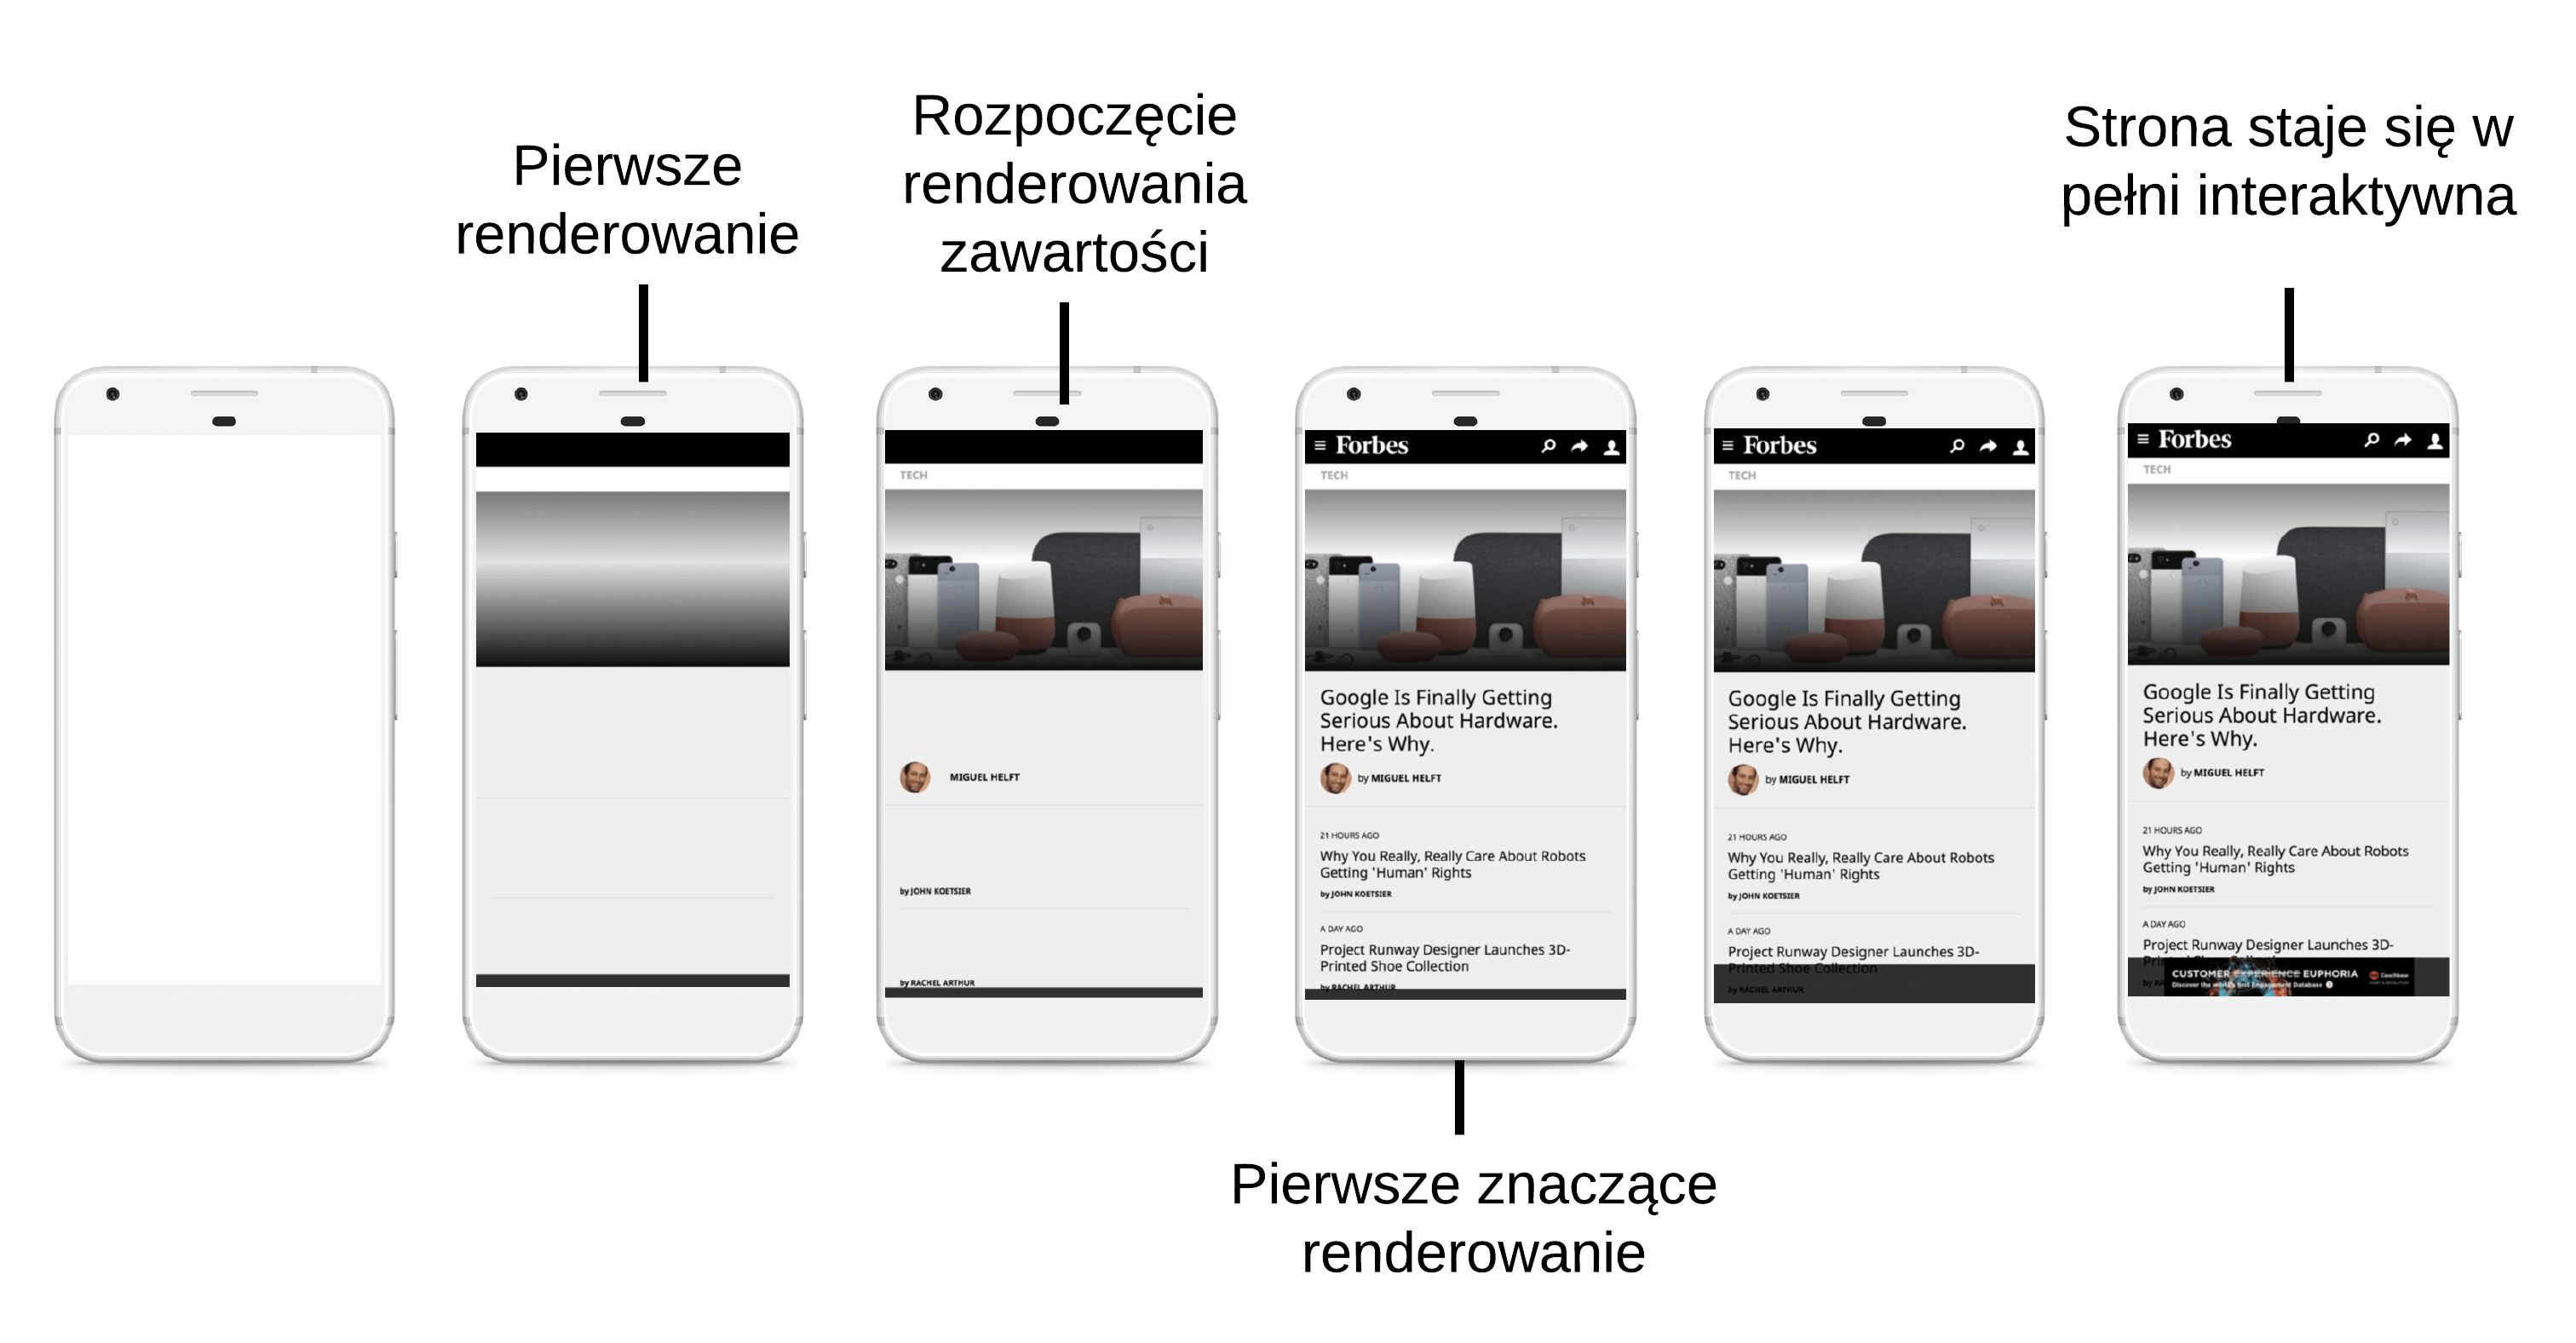
\includegraphics[width=12cm]{rysunek_20.png}
%     \caption{Ilustracja procesu ładowania aplikacji oraz zdarzenia rejestrowane przez przeglądarkę}
%     \label{fig:rysunek_20}
% \end{figure}

% \begin{figure}[!ht]
%     \centering
%     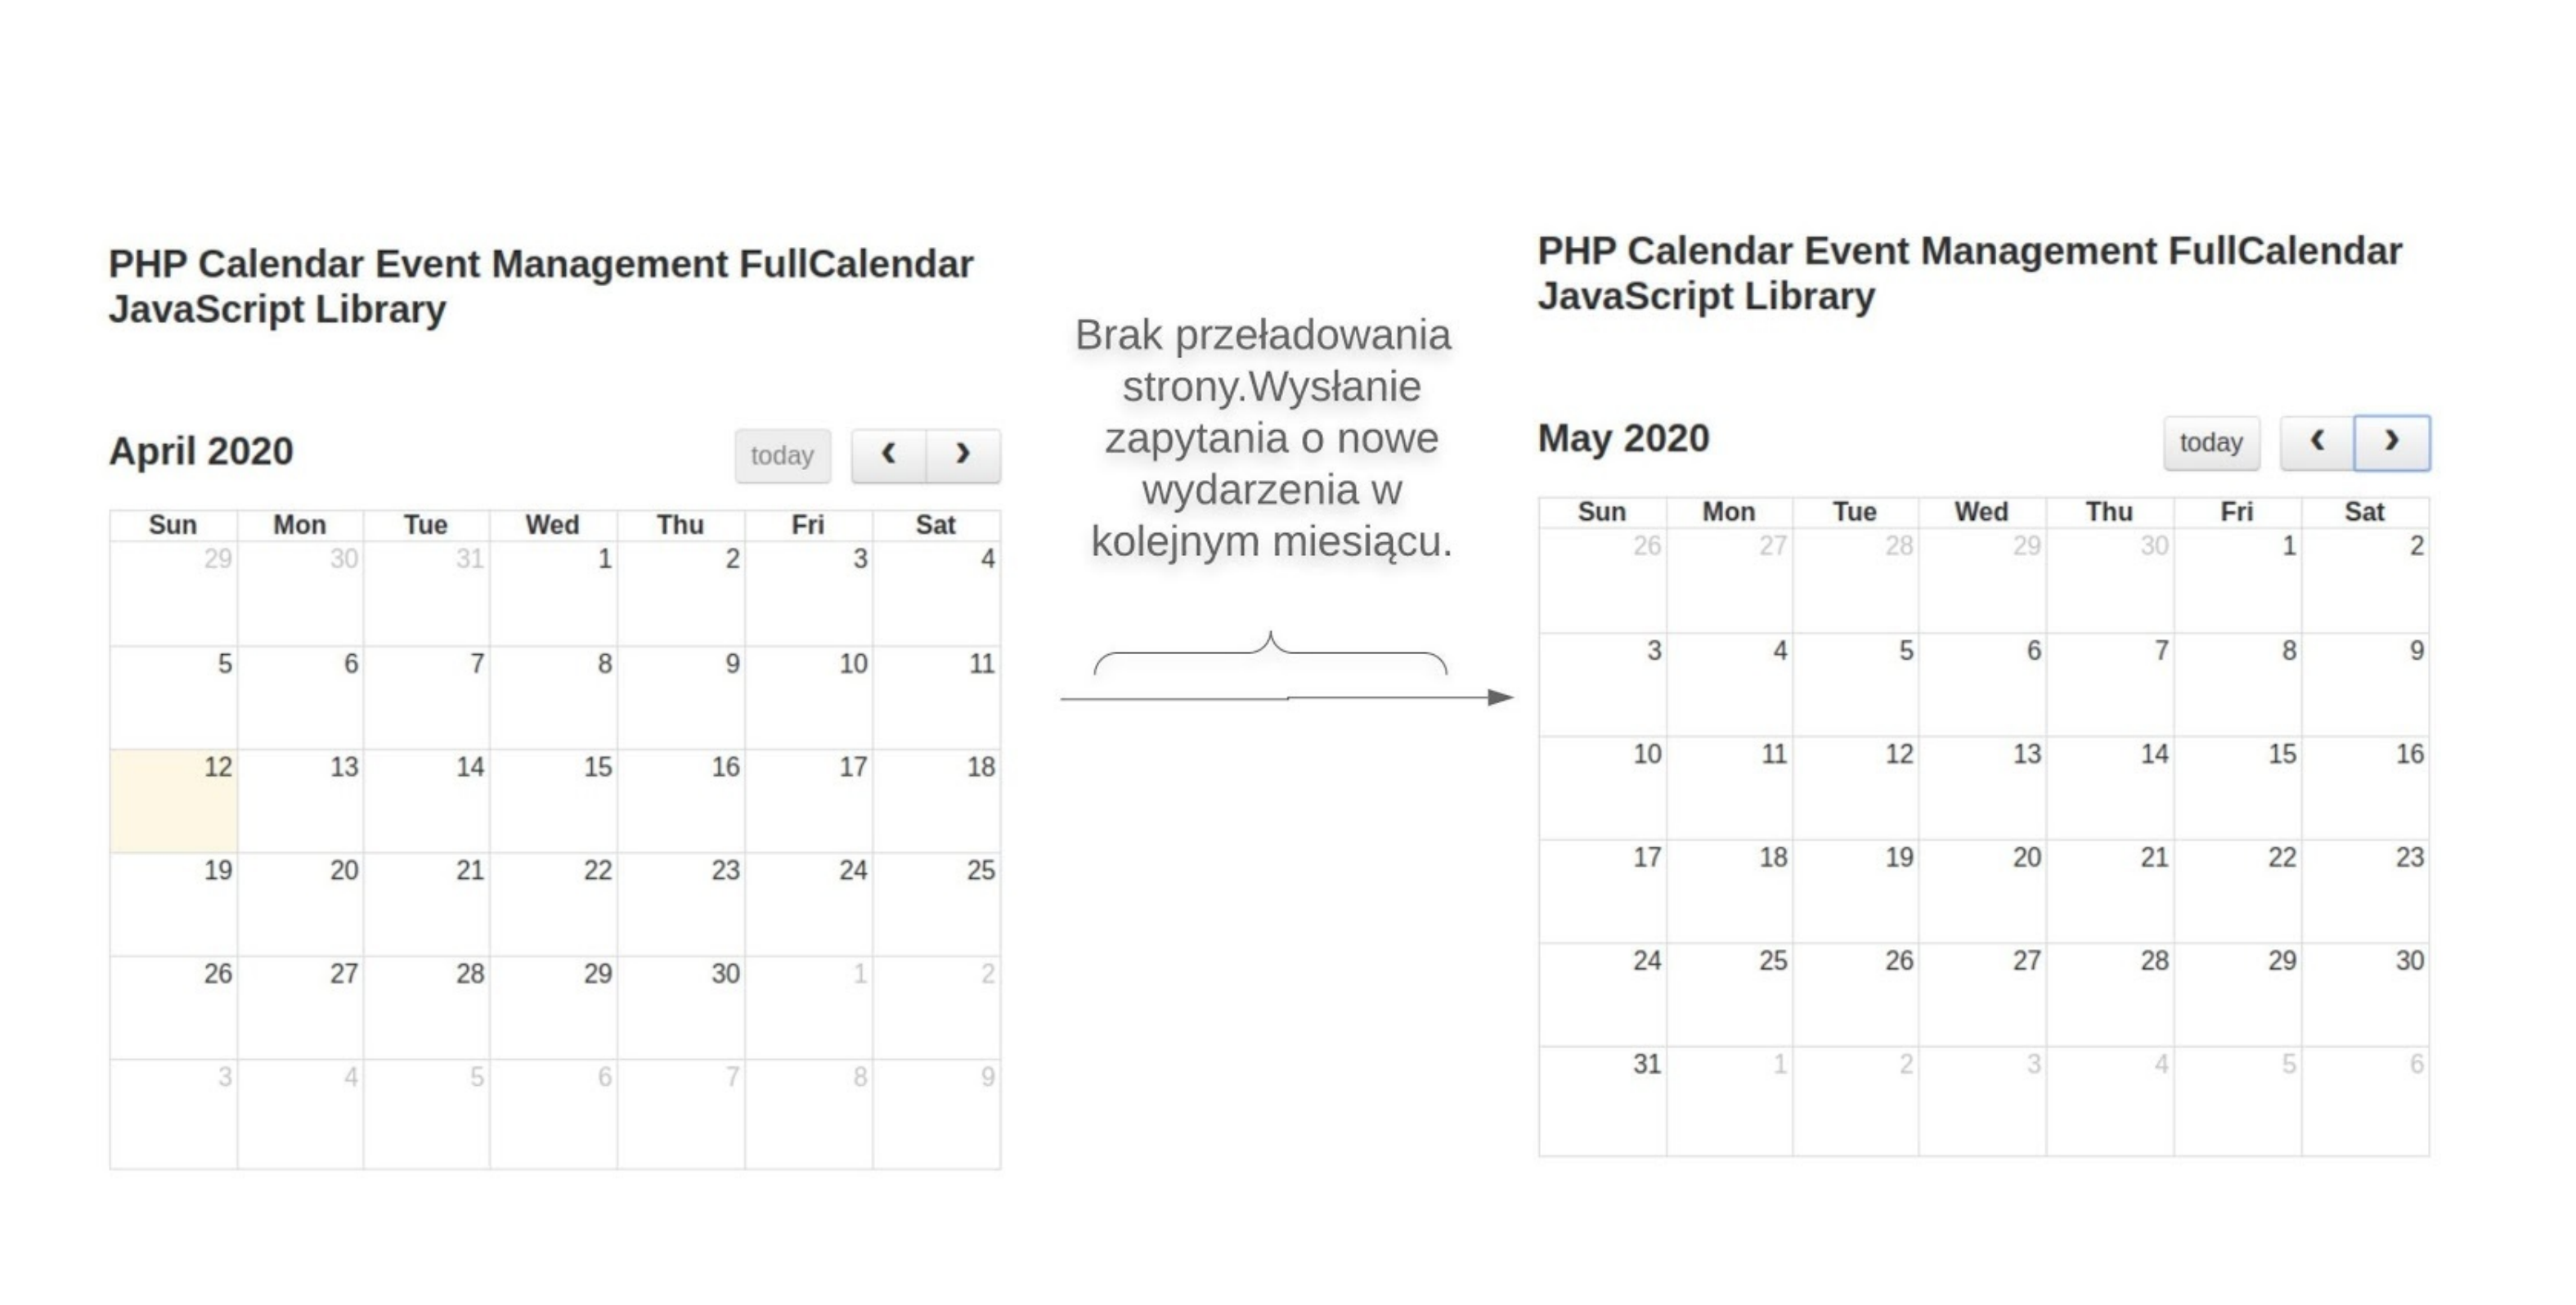
\includegraphics[width=12cm]{rysunek_21.png}
%     \caption{Ilustracja mechanizmu zmiany daty w przypadku aplikacji dynamicznej}
%     \label{fig:rysunek_21}
% \end{figure}

% \begin{figure}[!ht]
%     \centering
%     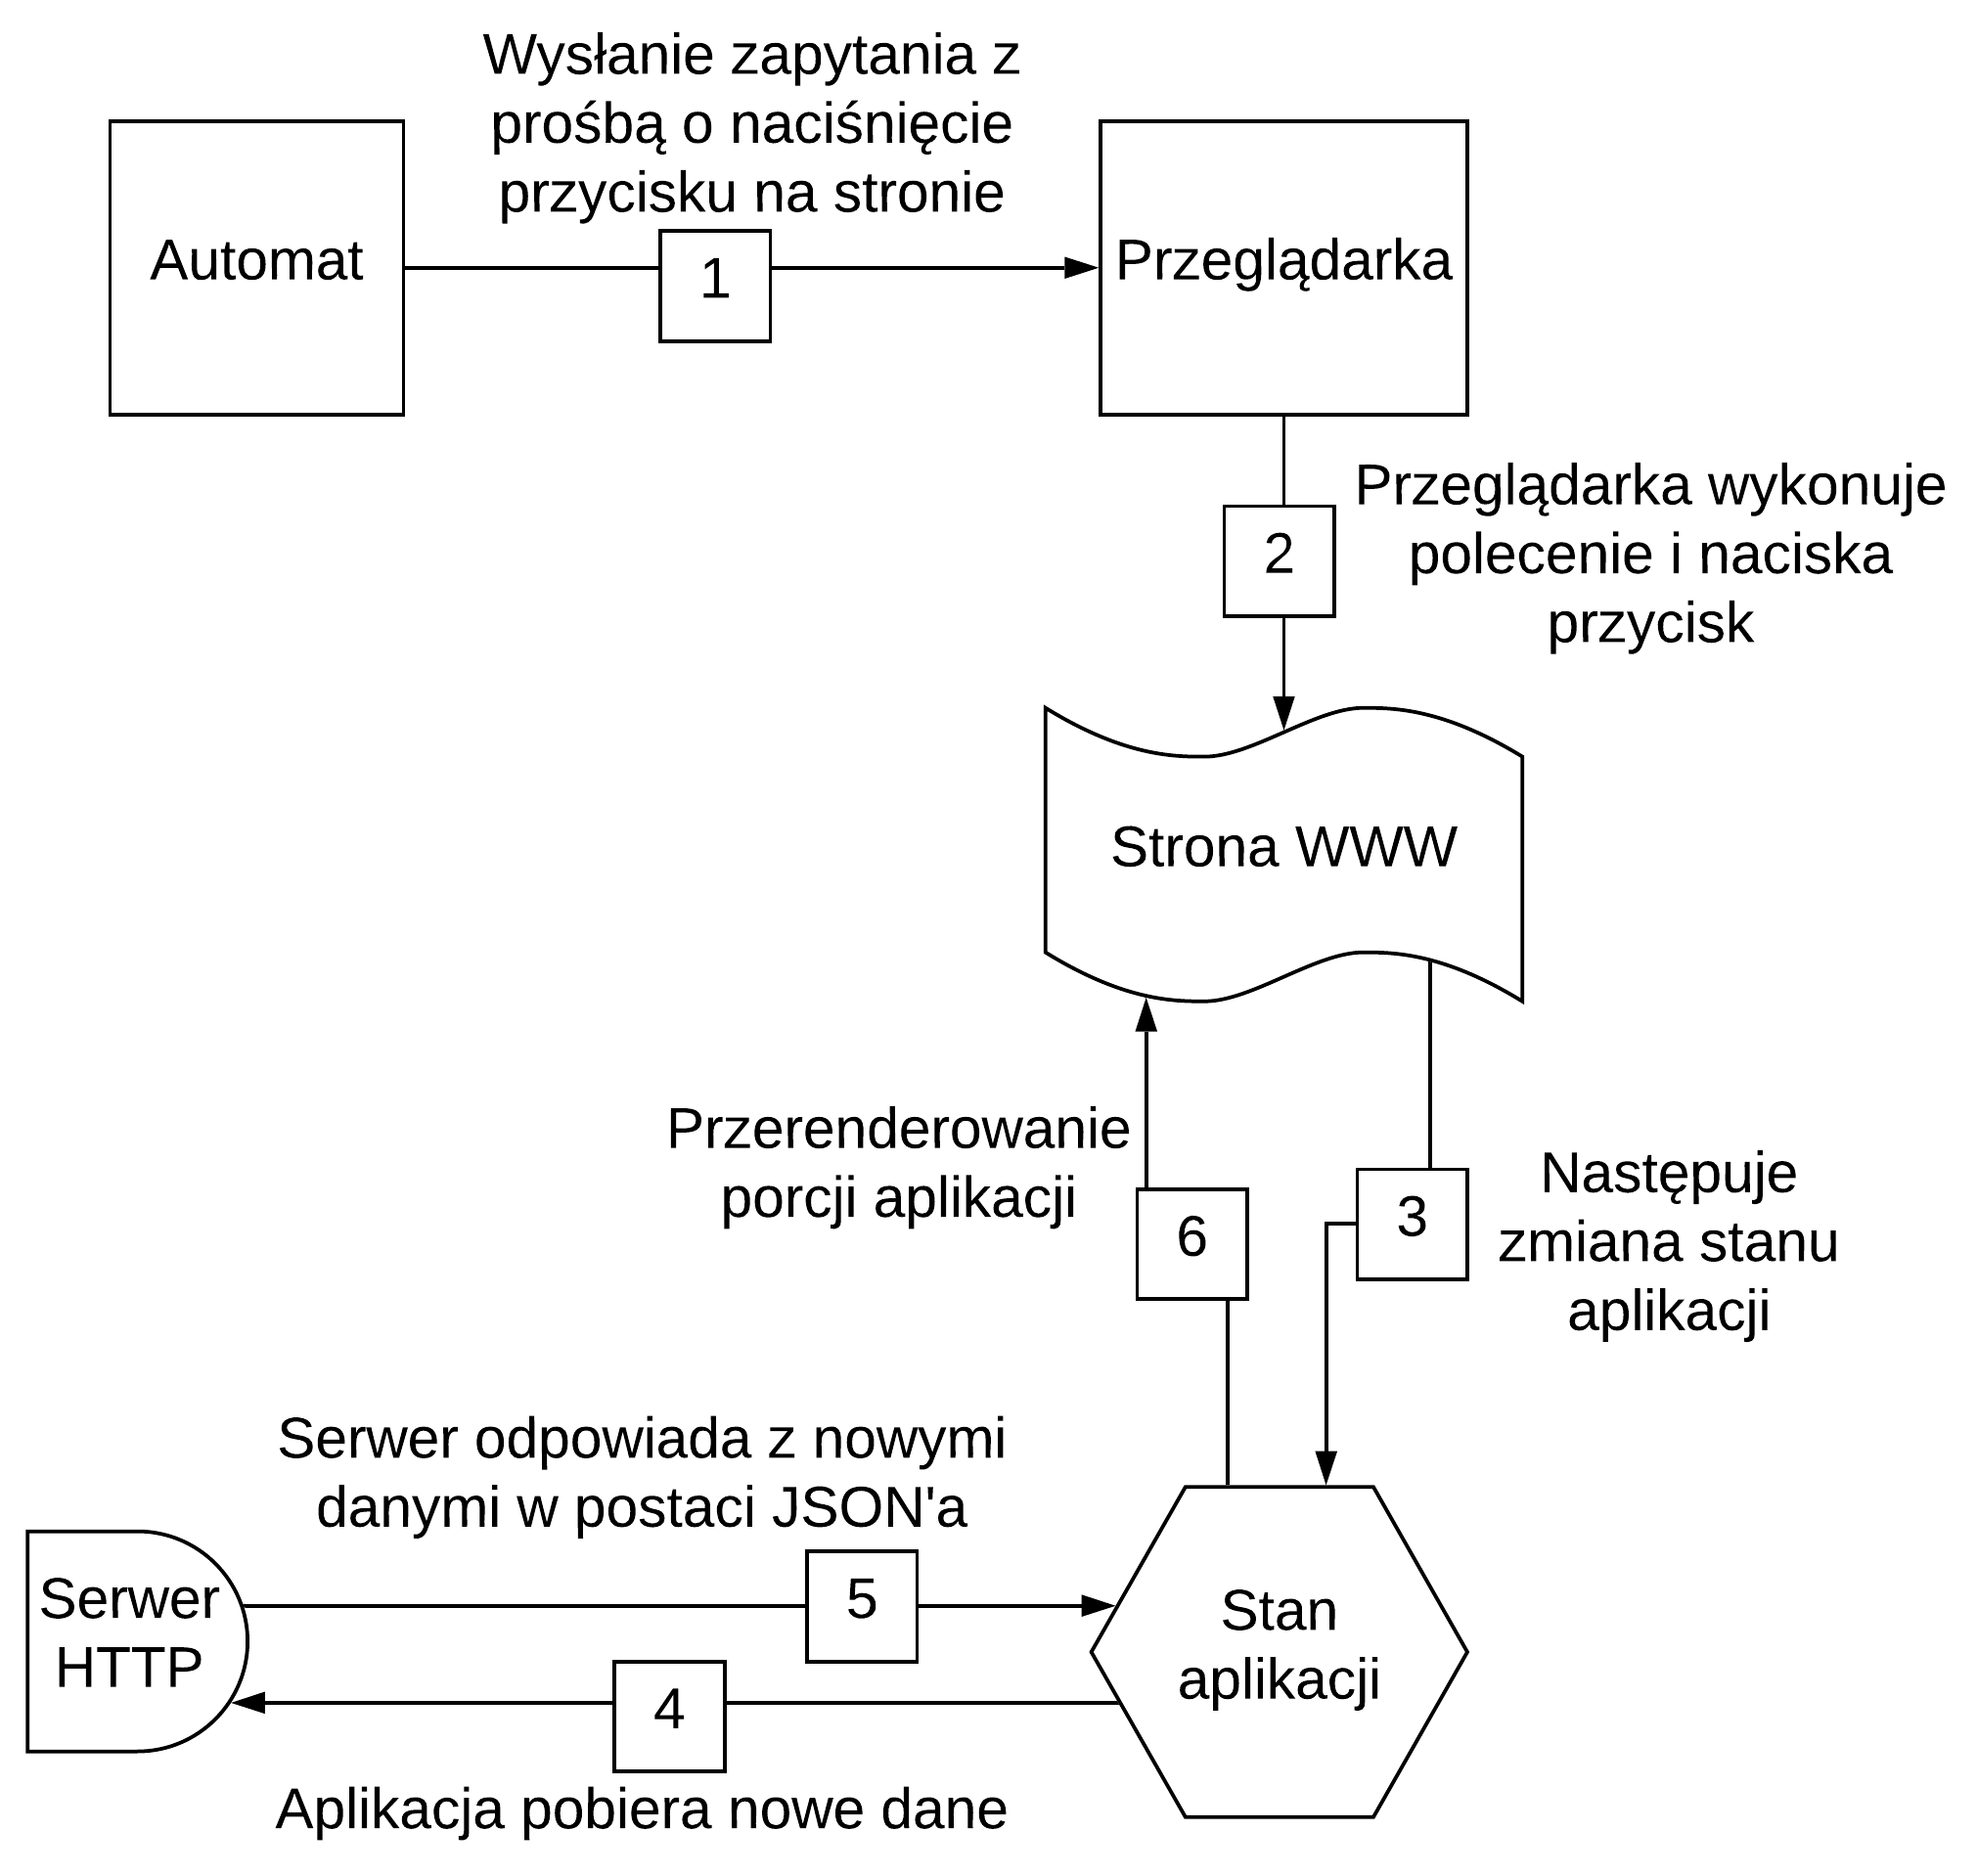
\includegraphics[width=12cm]{rysunek_22.png}
%     \caption{Ilustracja przedstawiająca proces zmiany treści strony w przypadku aplikacji dynamicznej}
%     \label{fig:rysunek_22}
% \end{figure}

% \begin{figure}[!ht]
%     \centering
%     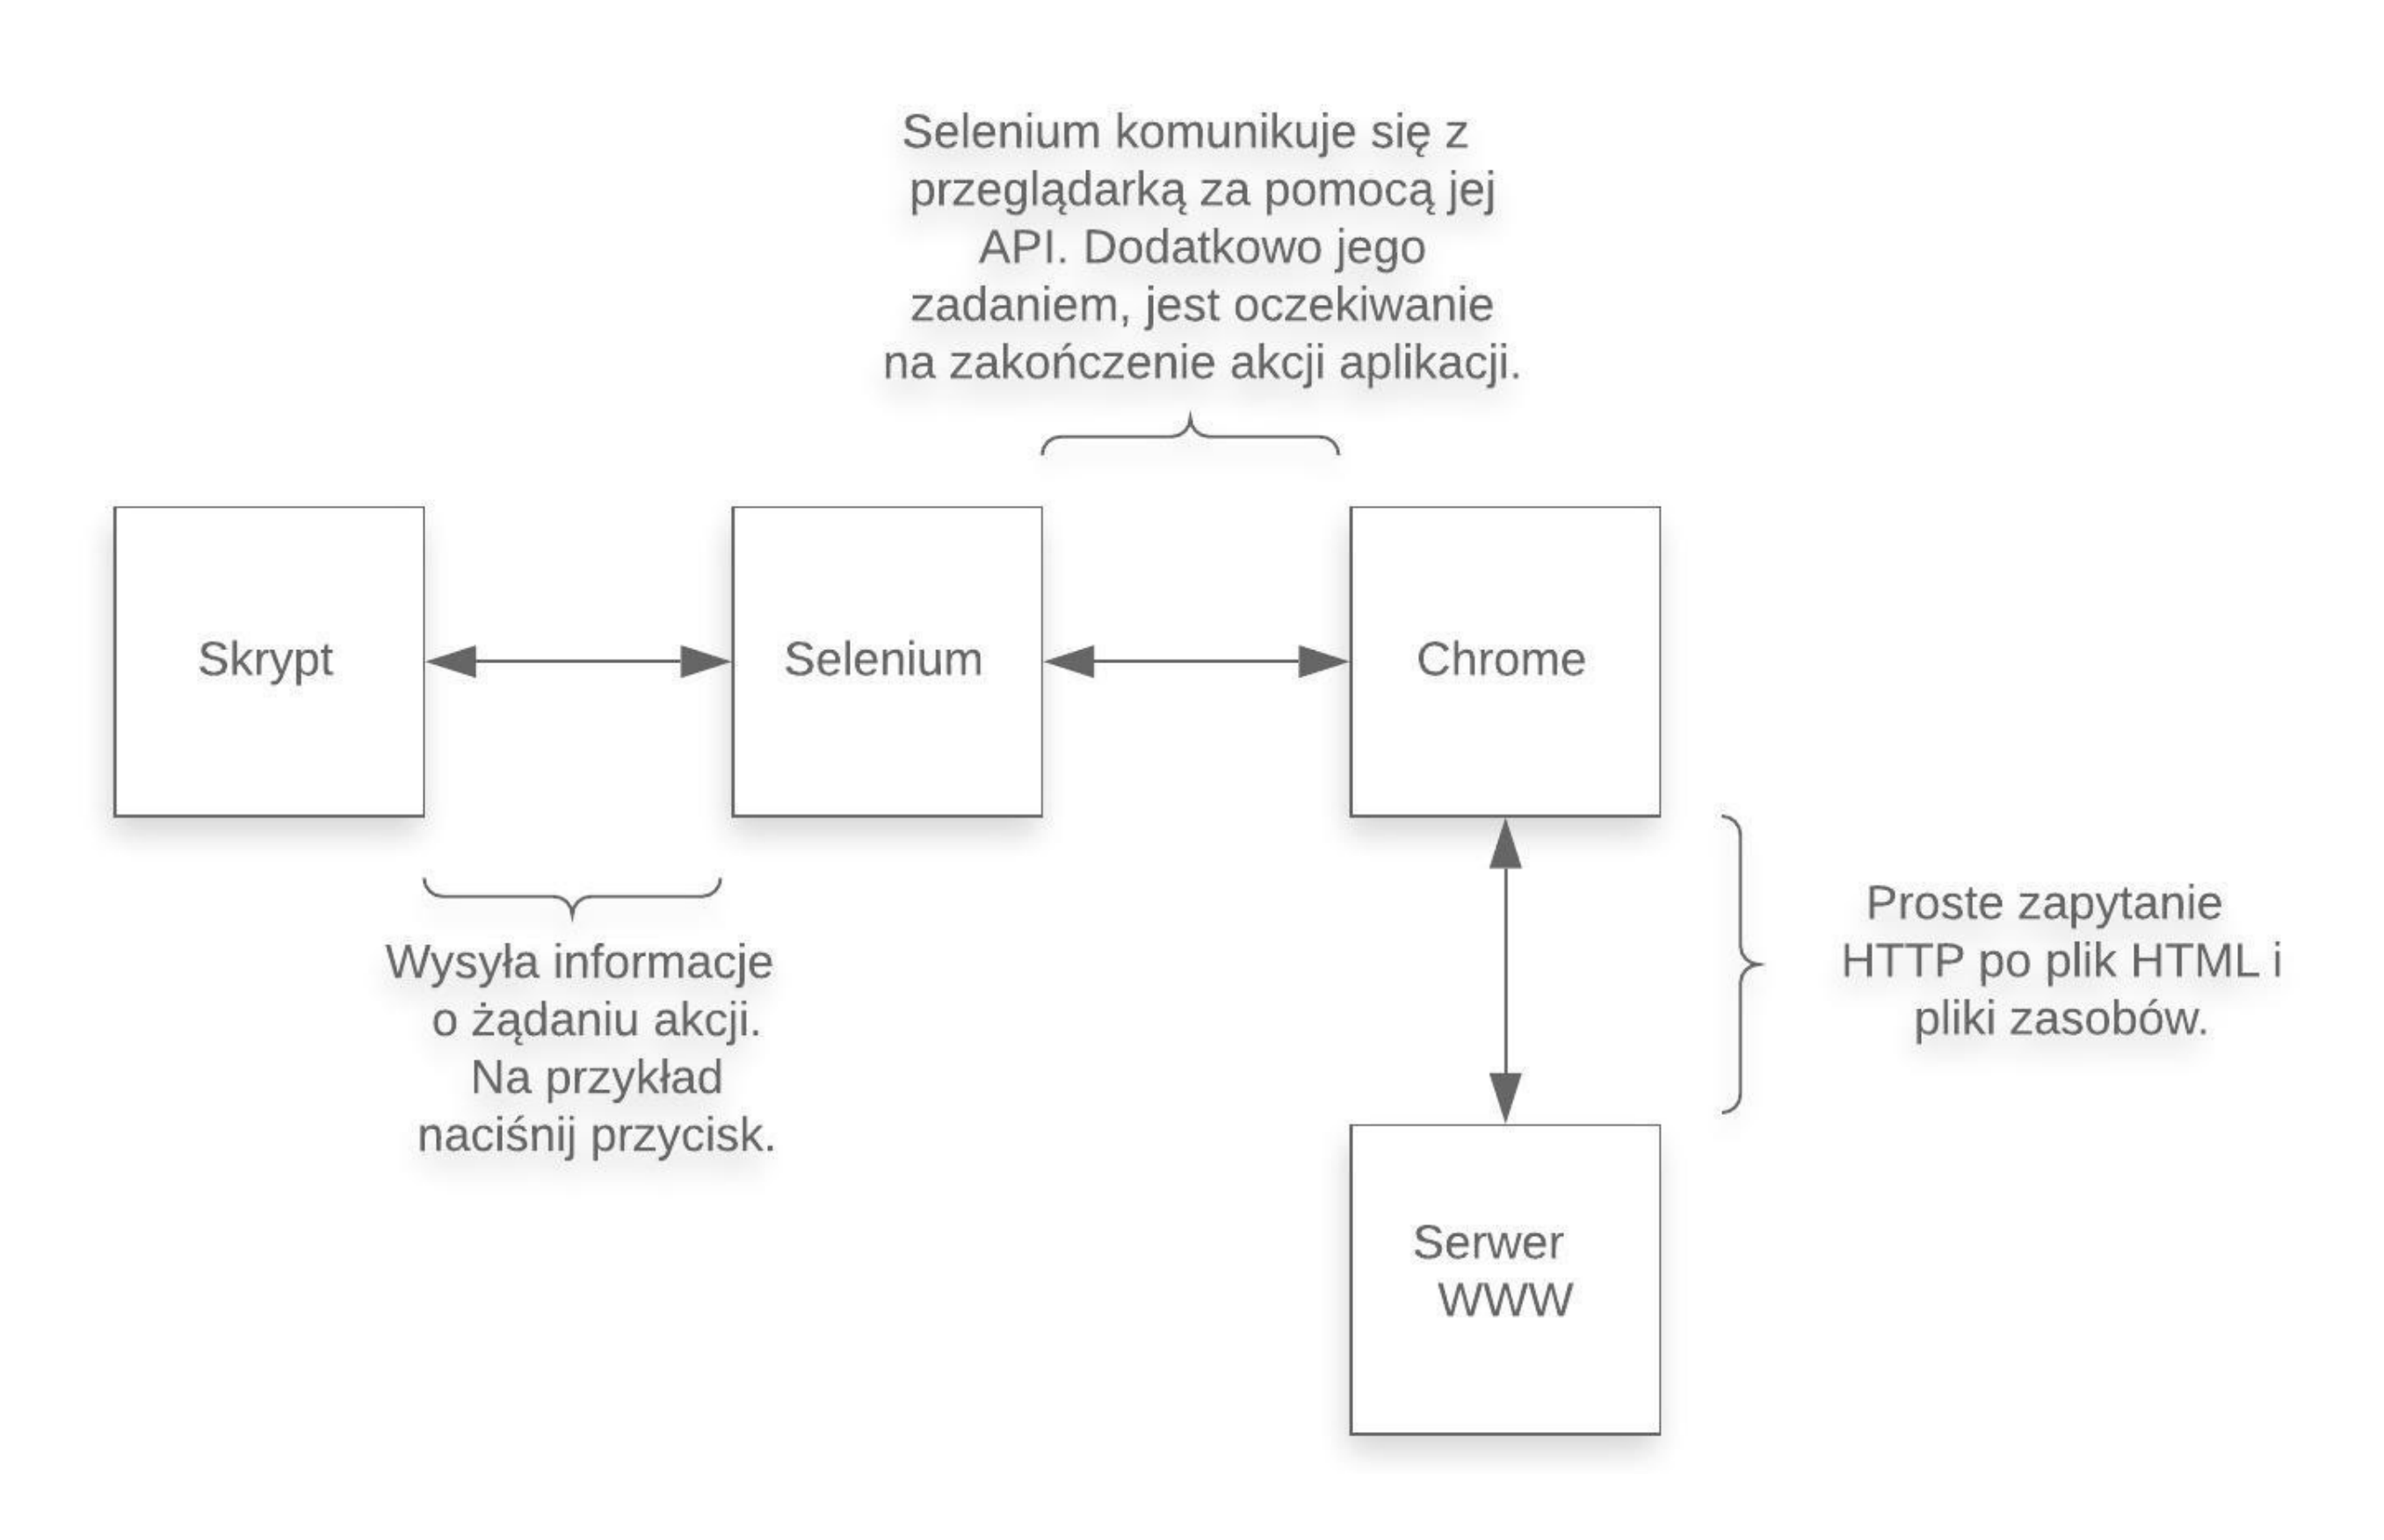
\includegraphics[width=12cm]{rysunek_23.png}
%     \caption{Ilustracja procesu współpracy pomiędzy Selenium a przeglądarką}
%     \label{fig:rysunek_23}
% \end{figure}

% \begin{figure}[!ht]
%     \centering
%     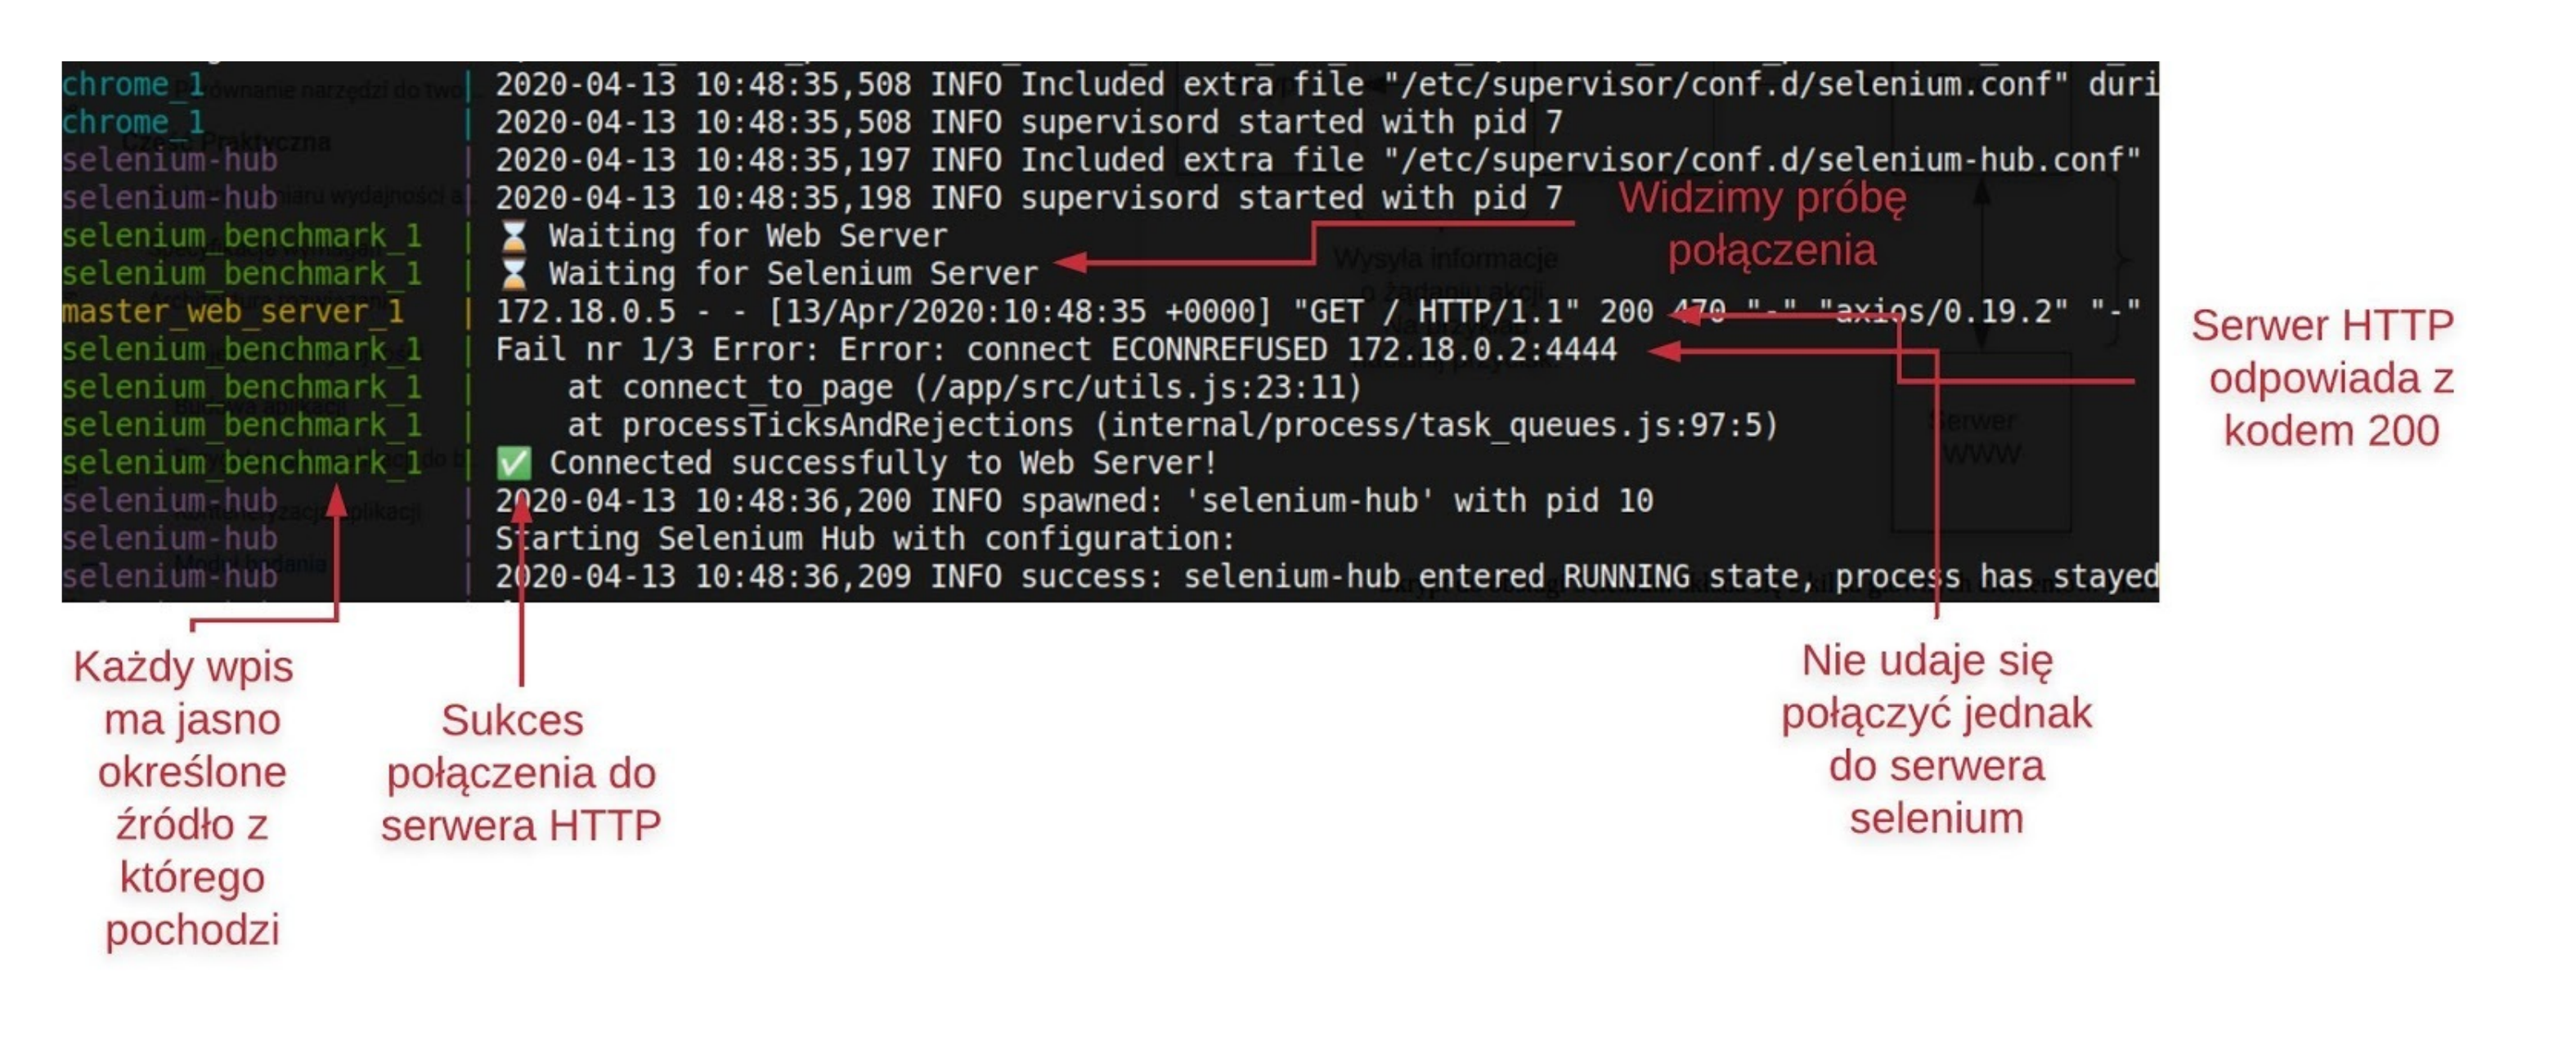
\includegraphics[width=12cm]{rysunek_24.png}
%     \caption{Wycinek wpisów skryptu przeprowadzającego badanie w środowisku docker-compose. Ilustruje on inicjalizację skryptu oraz mechanizm uzyskiwania połączenia pomiędzy Skryptem - Przeglądarką - Selenium}
%     \label{fig:rysunek_24}
% \end{figure}

% \begin{figure}[!ht]
%     \centering
%     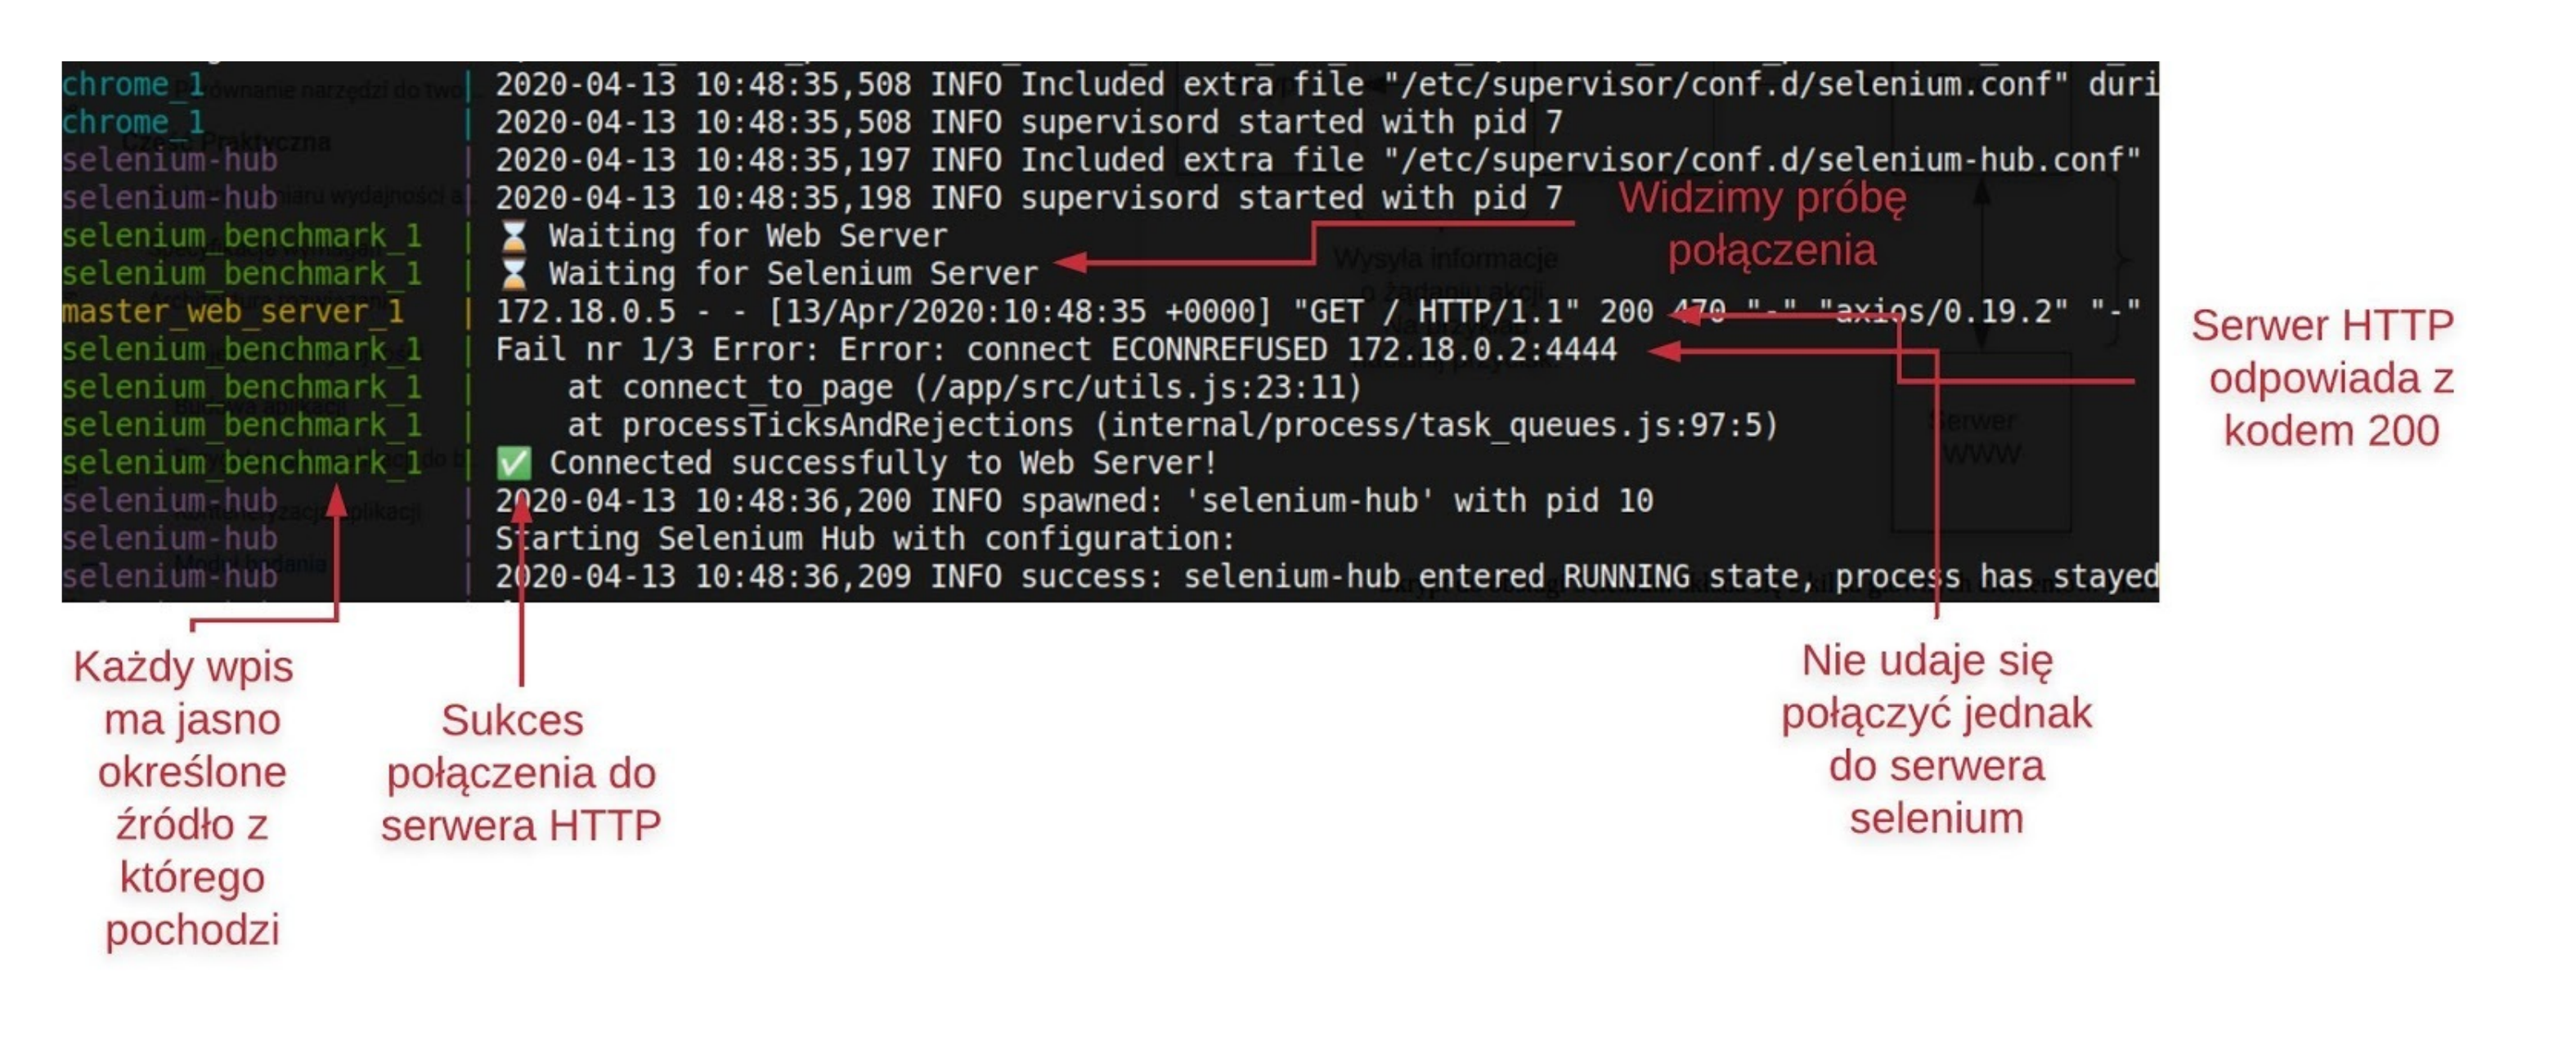
\includegraphics[width=12cm]{rysunek_25.png}
%     \caption{Wycinek skryptu ukazujący uzyskanie połączenia do Selenium pomimo początkowych problemów}
%     \label{fig:rysunek_25}
% \end{figure}

% \begin{figure}[!ht]
%     \centering
%     \includegraphics[width=12cm]{rysunek_26.png}
%     \caption{Grafika przedstawia rozpoczęcie badania}
%     \label{fig:rysunek_26}
% \end{figure}

% \begin{figure}[!ht]
%     \centering
%     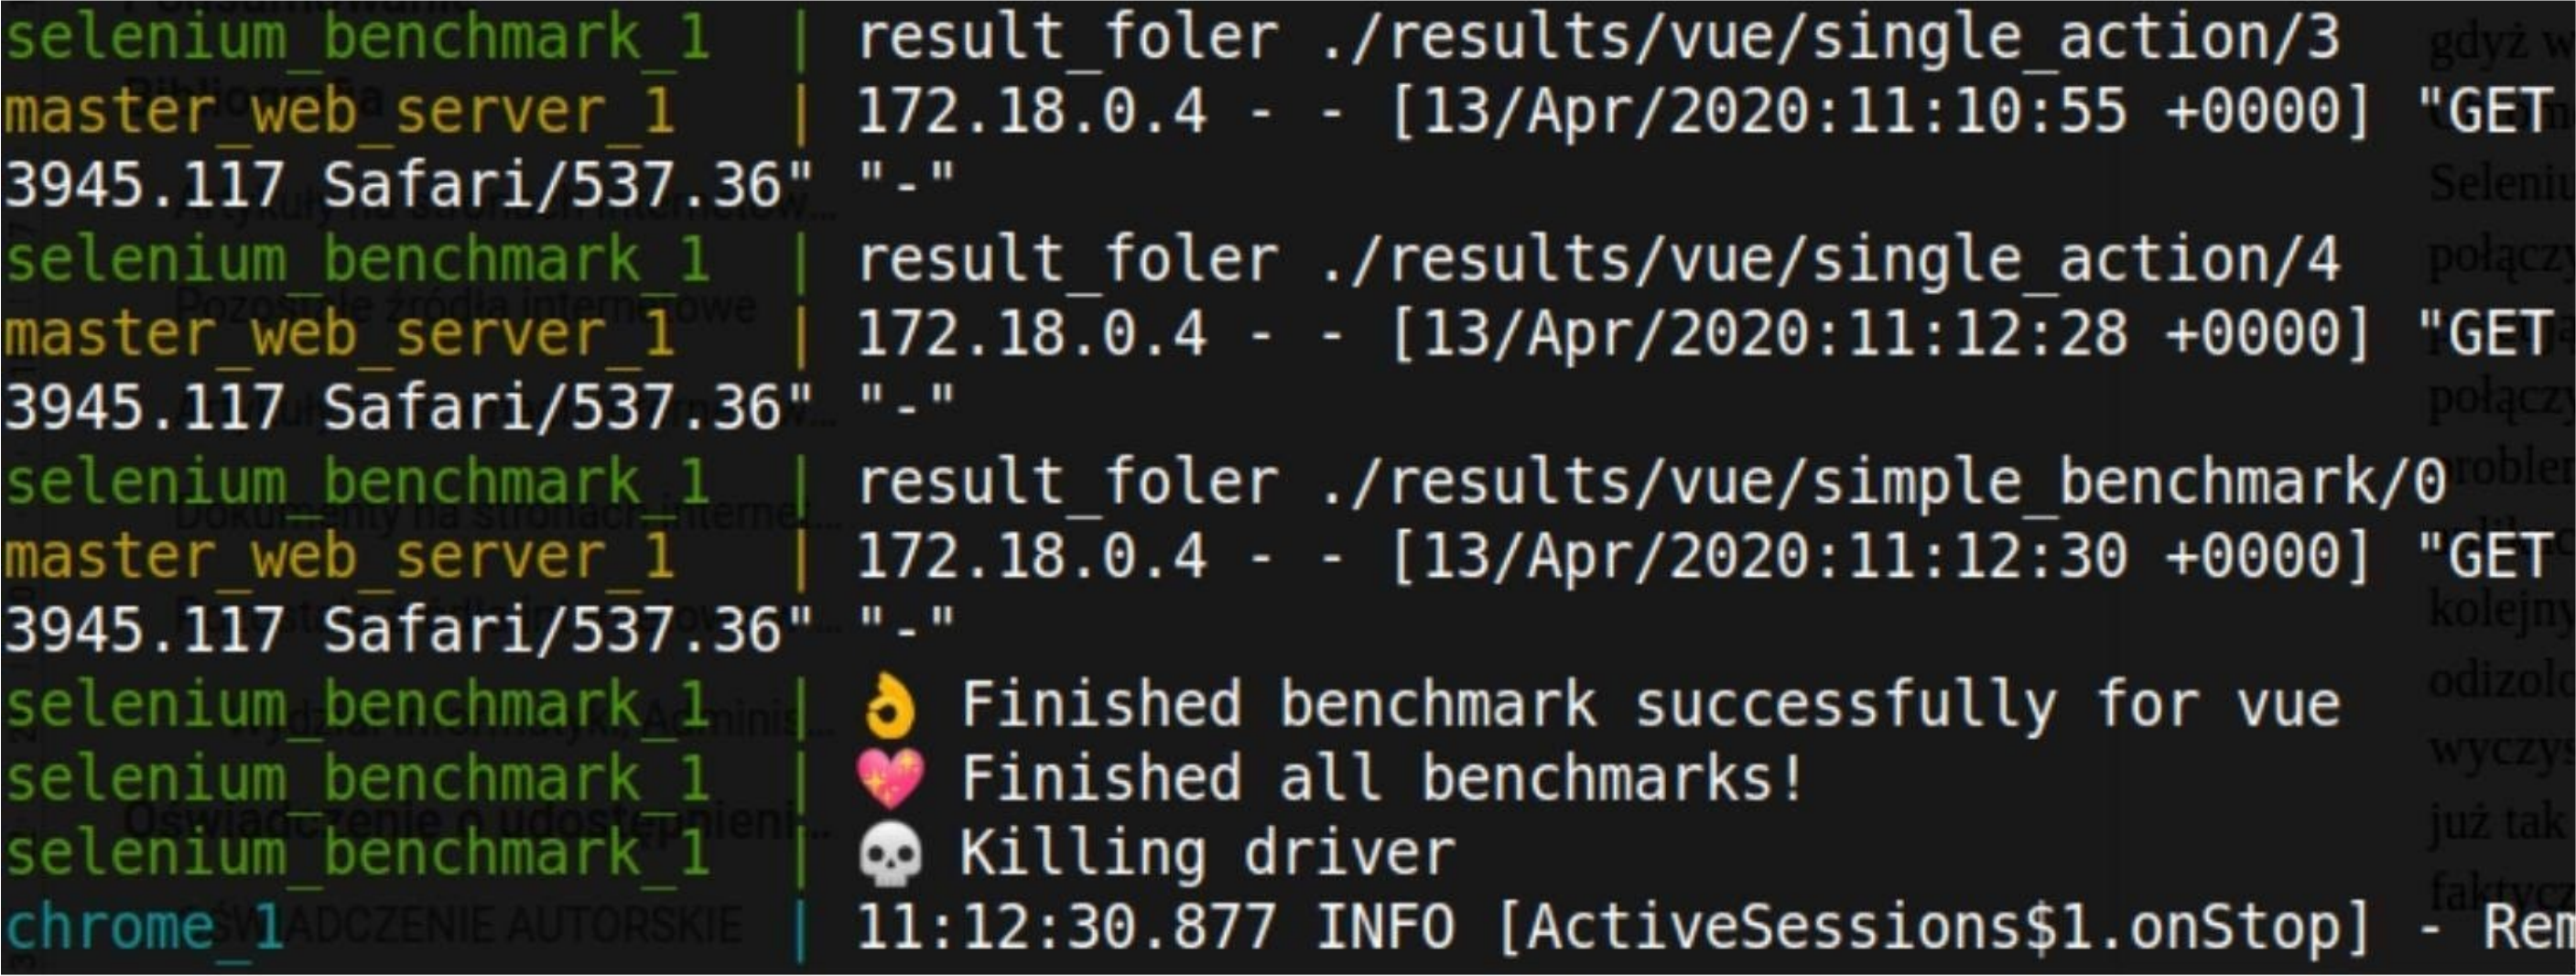
\includegraphics[width=12cm]{rysunek_27.png}
%     \caption{Grafika przedstawia skrypt zakańczający badanie po zapisaniu zebranych danych na dysk - widzimy, że ważnym elementem jest zamknięcie połączenia do Selenium}
%     \label{fig:rysunek_27}
% \end{figure}

% \begin{figure}[!ht]
%     \centering
%     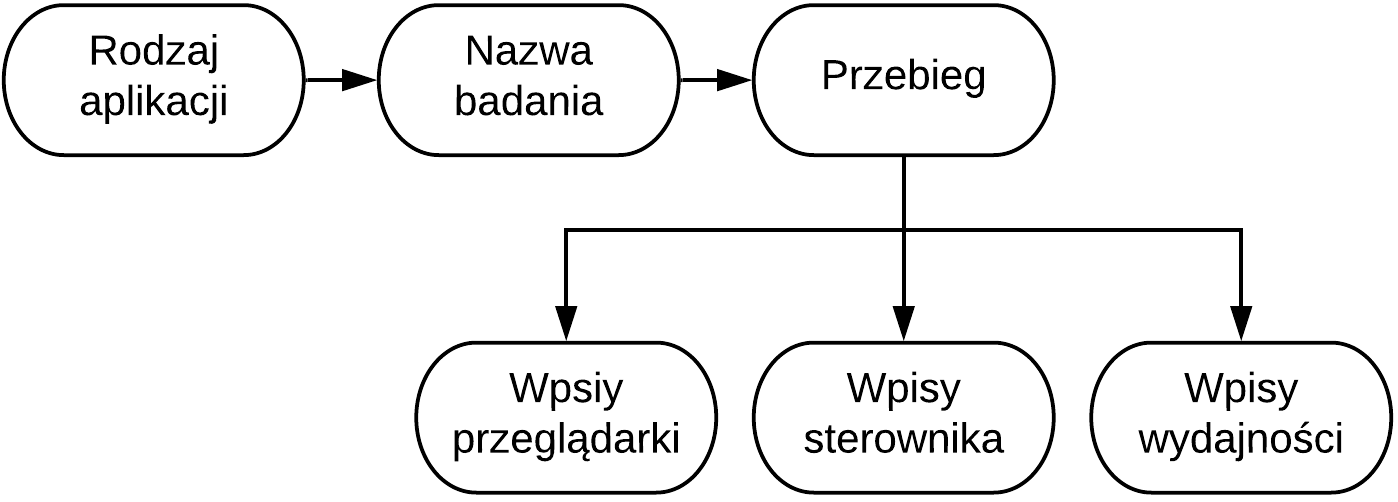
\includegraphics[width=12cm]{rysunek_28.png}
%     \caption{Ilustracja struktury wyniku badania na które zostanie poddane dalszej obróbce}
%     \label{fig:rysunek_28}
% \end{figure}

% \begin{figure}[!ht]
%     \centering
%     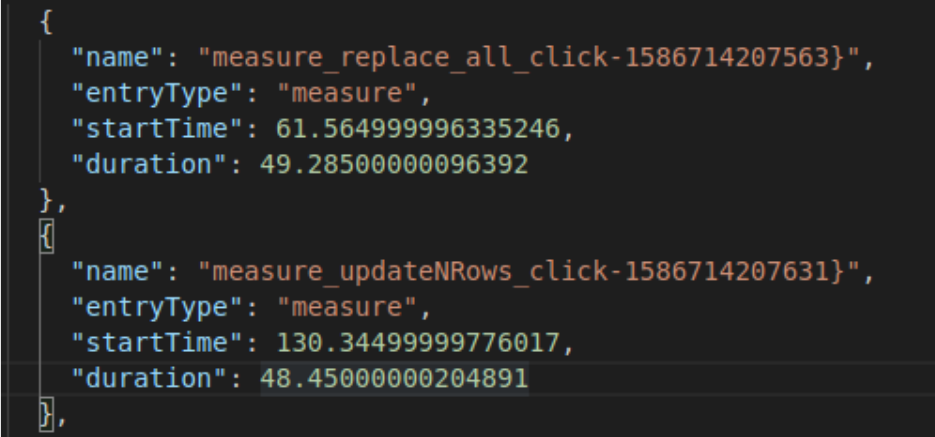
\includegraphics[width=12cm]{rysunek_29.png}
%     \caption{Grafika przedstawiająca wpis zebranego pomiaru}
%     \label{fig:rysunek_29}
% \end{figure}

% \begin{figure}[!ht]
%     \centering
%     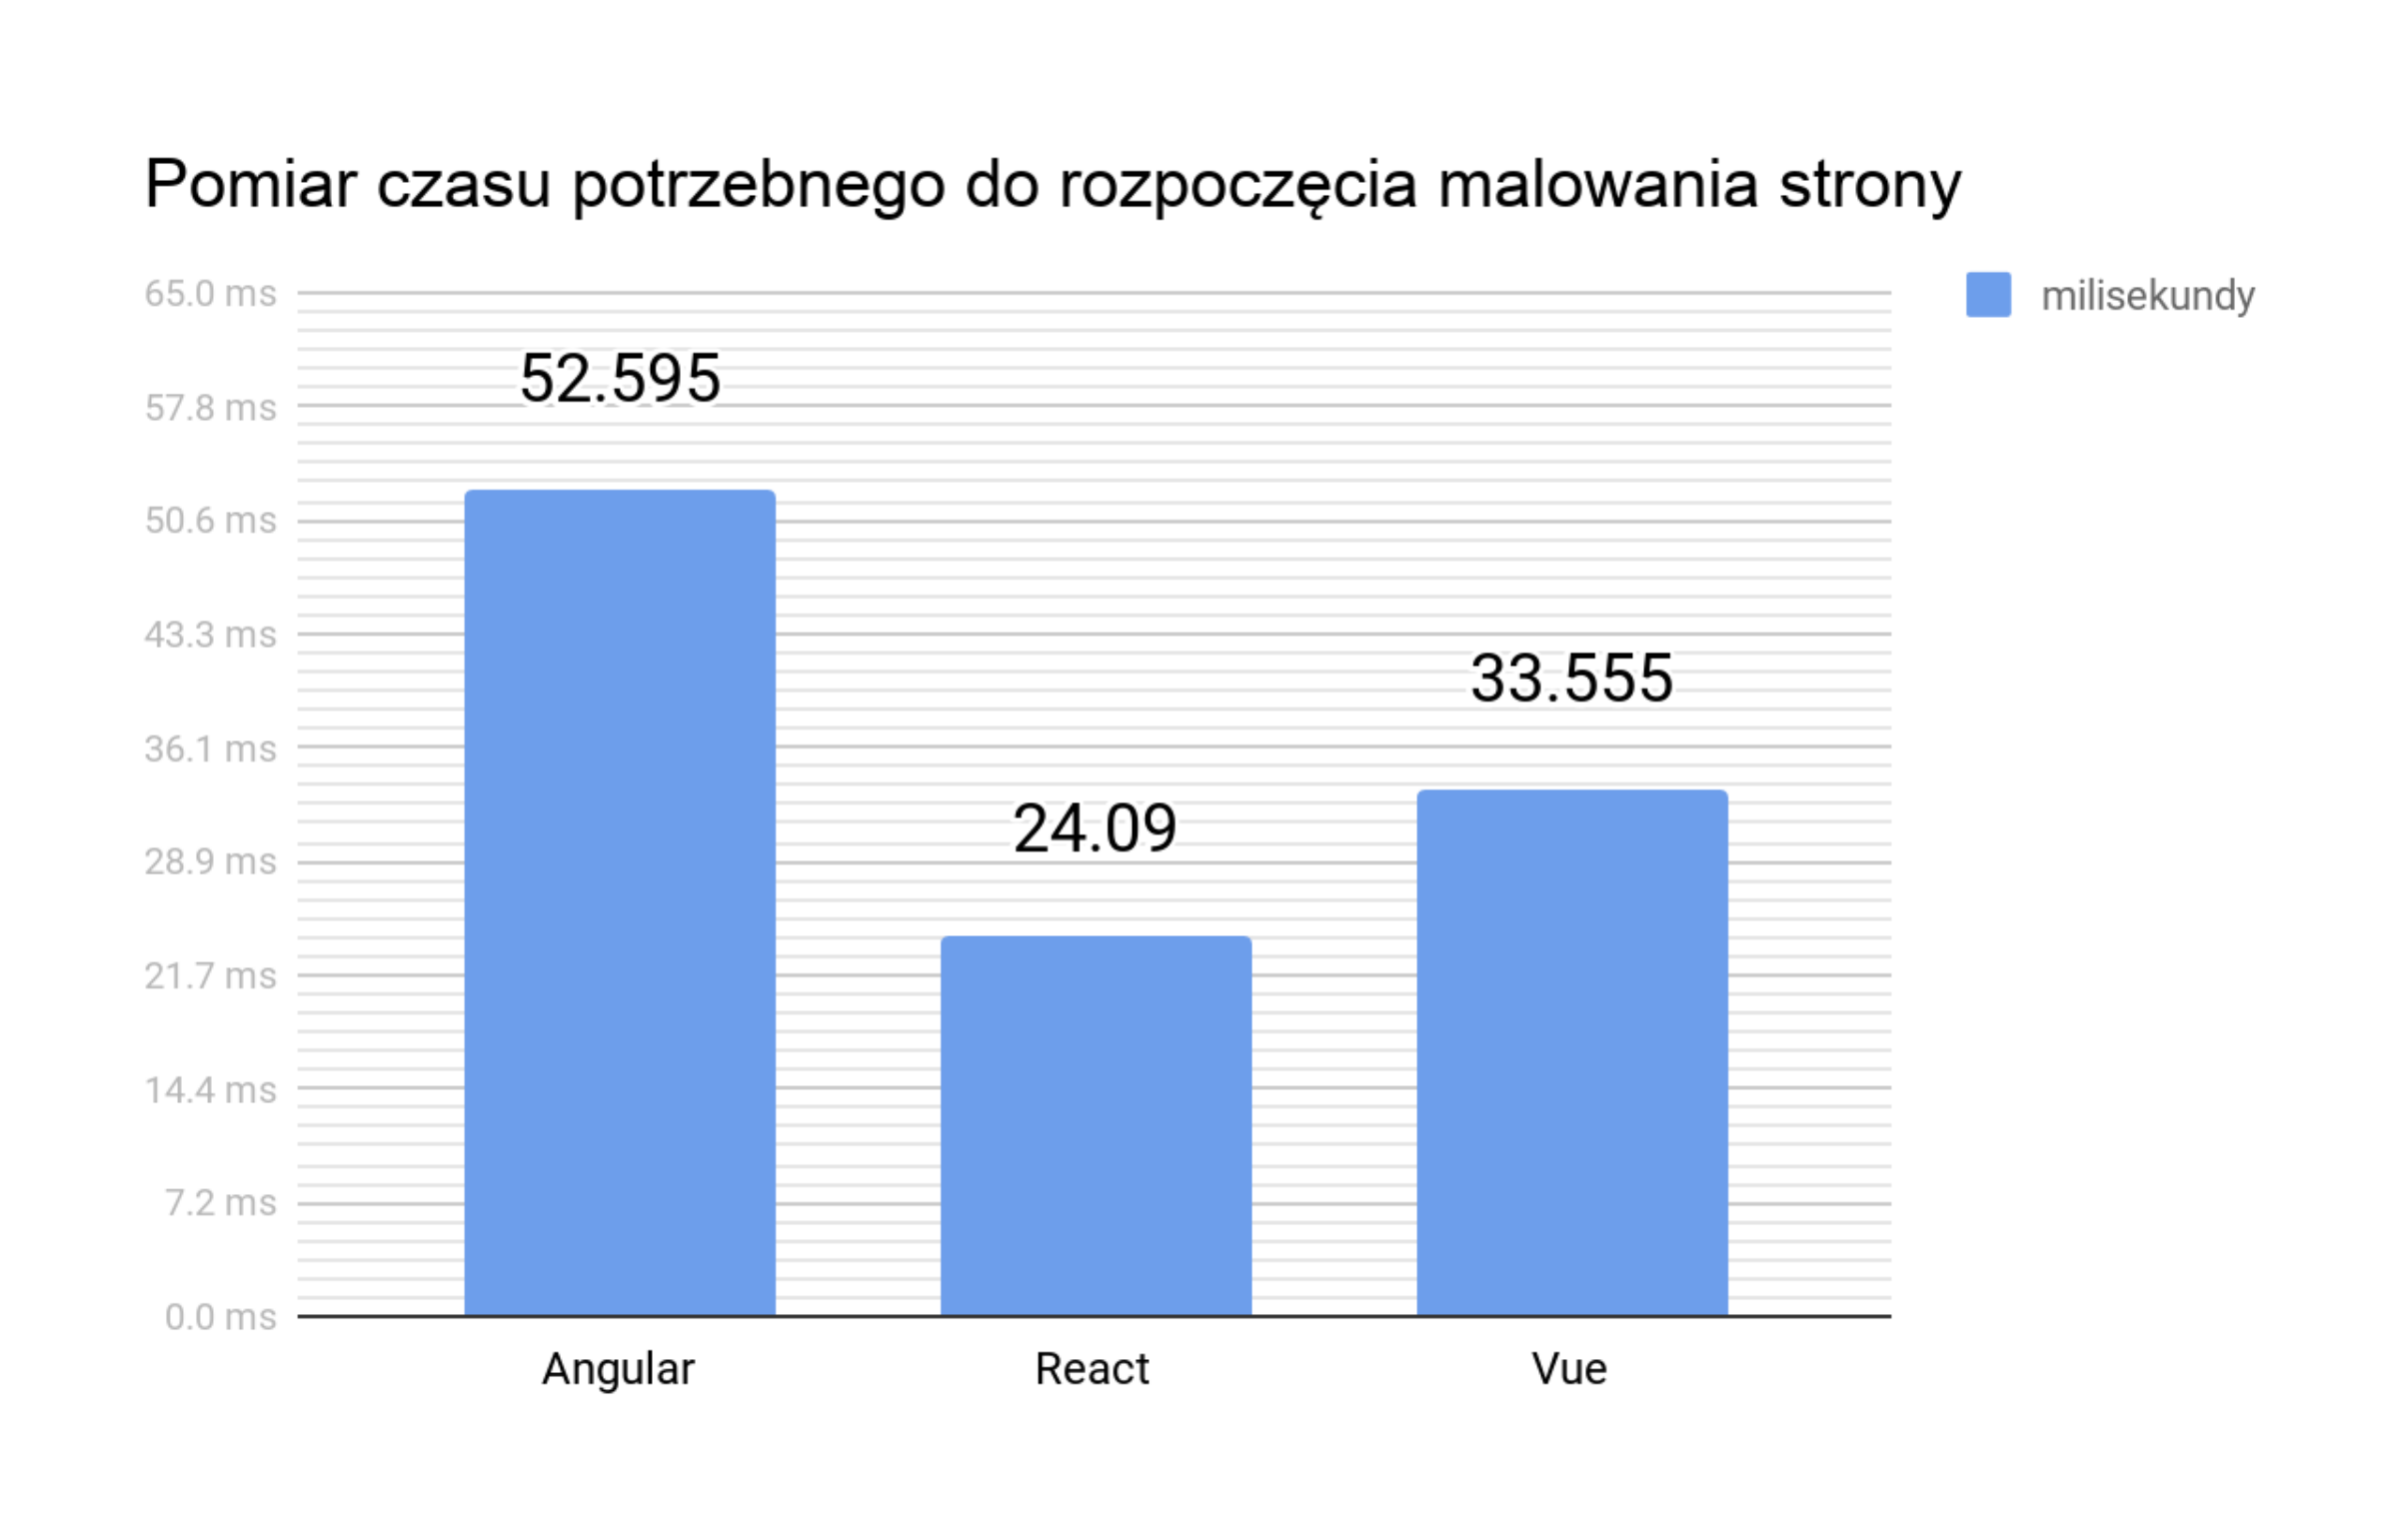
\includegraphics[width=12cm]{rysunek_30.png}
%     \caption{Diagram kolumnowy ukazujący wynik badania czasu potrzebnego do rozpoczęcia malowania strony}
%     \label{fig:rysunek_30}
% \end{figure}

% \begin{figure}[!ht]
%     \centering
%     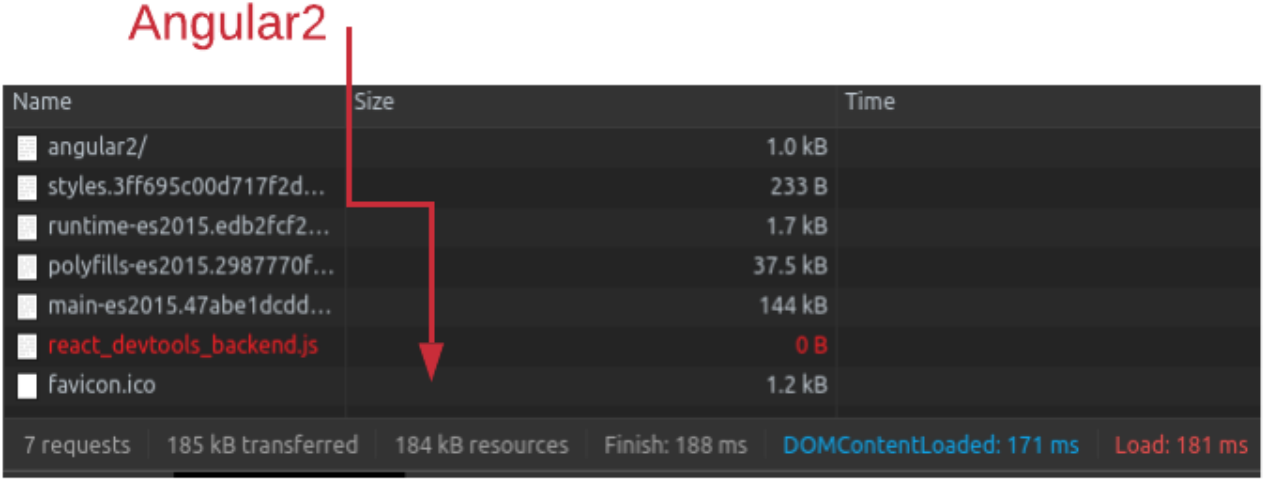
\includegraphics[width=12cm]{rysunek_31.png}
%     \caption{Grafika ukazująca rozmiar plików zasobów dla aplikacji Angular2}
%     \label{fig:rysunek_31}
% \end{figure}

% \begin{figure}[!ht]
%     \centering
%     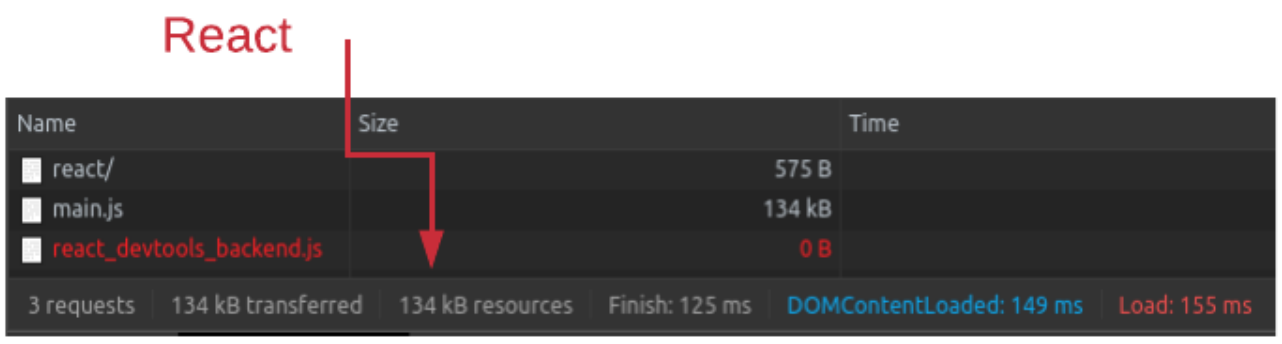
\includegraphics[width=12cm]{rysunek_32.png}
%     \caption{Grafika ukazująca rozmiar plików zasobów dla aplikacji React}
%     \label{fig:rysunek_32}
% \end{figure}

% \begin{figure}[!ht]
%     \centering
%     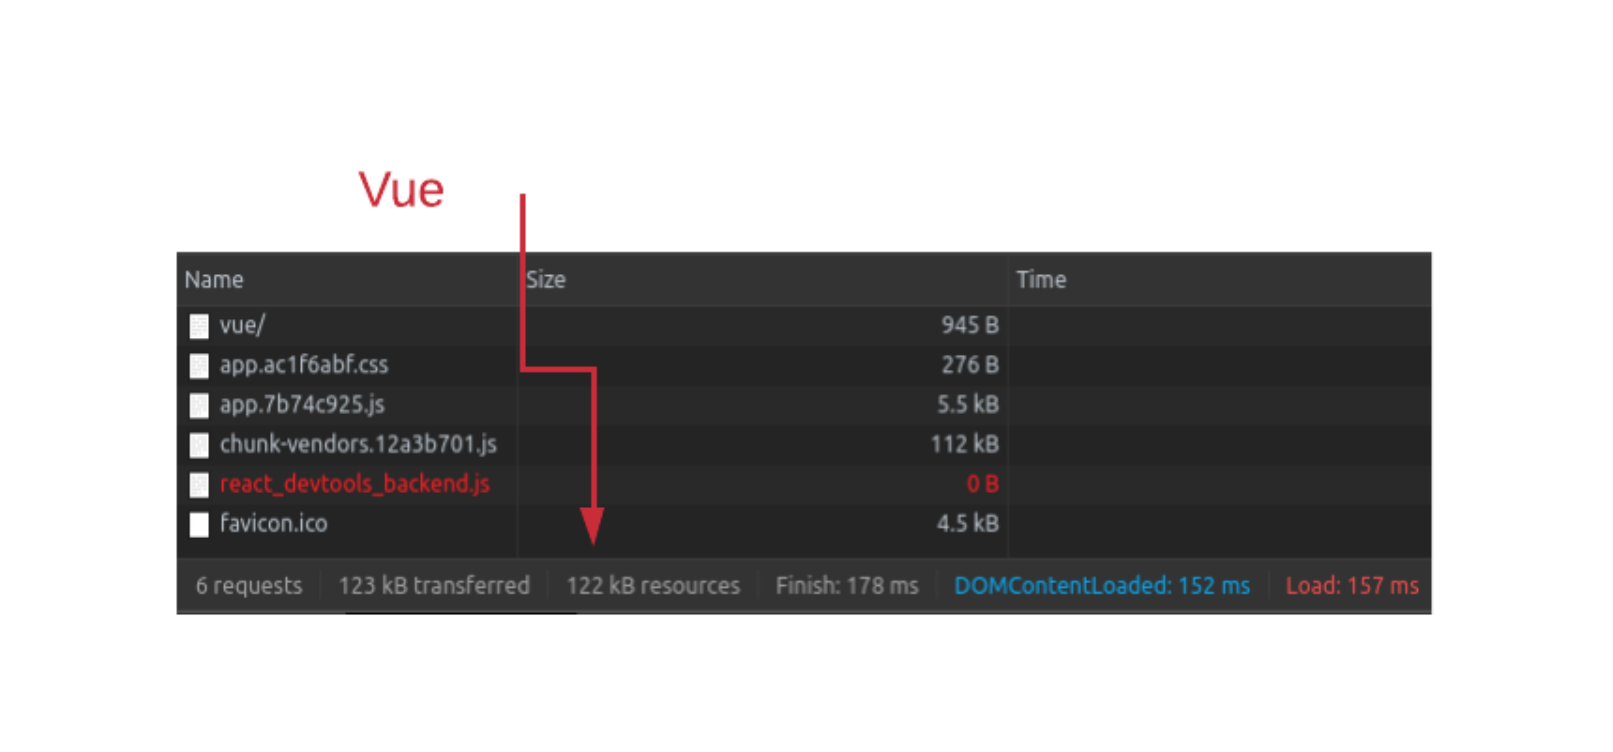
\includegraphics[width=12cm]{rysunek_33.png}
%     \caption{Grafika ukazująca rozmiar plików zasobów dla aplikacji Vue}
%     \label{fig:rysunek_33}
% \end{figure}

% \begin{figure}[!ht]
%     \centering
%     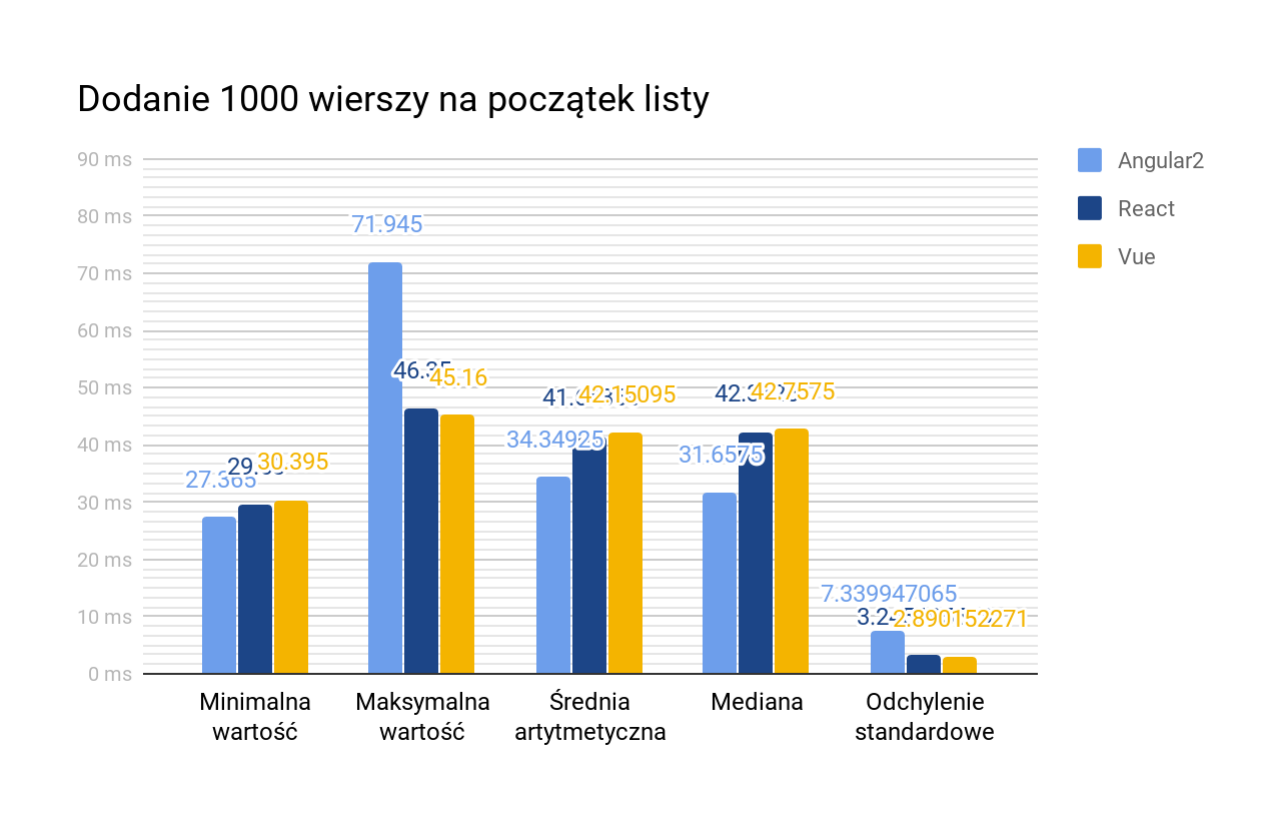
\includegraphics[width=12cm]{rysunek_34.png}
%     \caption{Diagram kolumnowy obrazujący wynik badania pomiaru czasu dodania 1000 elementów na początek listy}
%     \label{fig:rysunek_34}
% \end{figure}

% \begin{figure}[!ht]
%     \centering
%     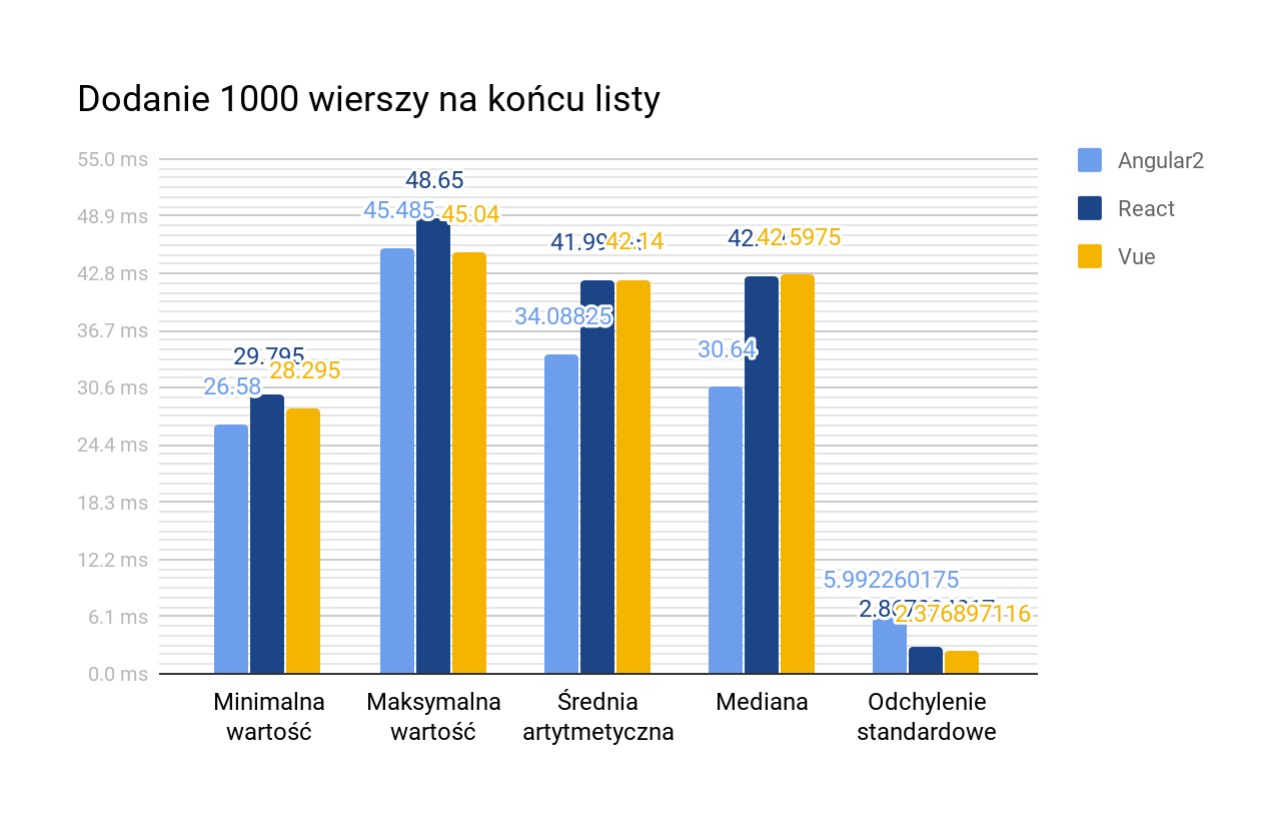
\includegraphics[width=12cm]{rysunek_35.png}
%     \caption{Diagram kolumnowy obrazujący wynik badania pomiaru czasu dodania 1000 elementów na koniec listy}
%     \label{fig:rysunek_35}
% \end{figure}

% \begin{figure}[!ht]
%     \centering
%     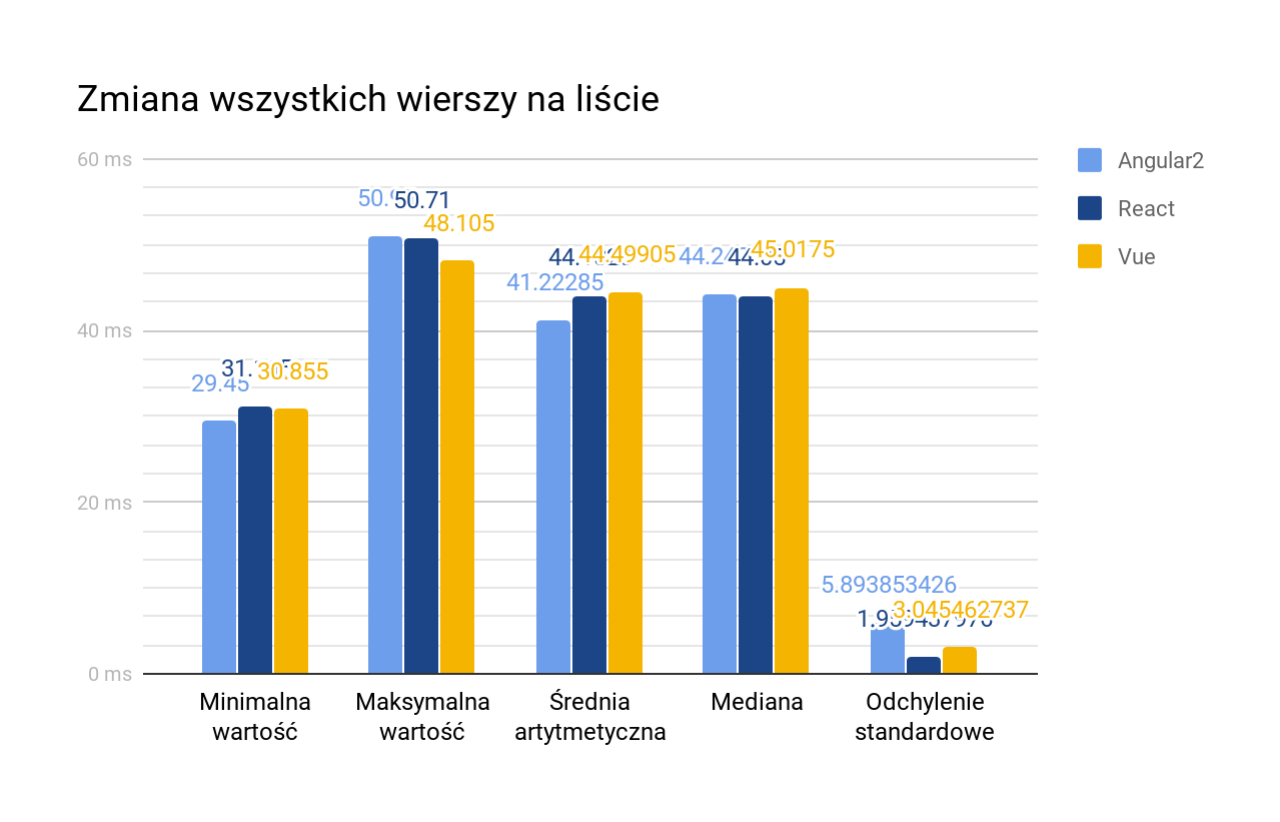
\includegraphics[width=12cm]{rysunek_36.png}
%     \caption{Diagram kolumnowy obrazujący wynik badania pomiaru czasu zmiany wszystkich wartości listy dla 1000 elementów}
%     \label{fig:rysunek_36}
% \end{figure}

% \begin{figure}[!ht]
%     \centering
%     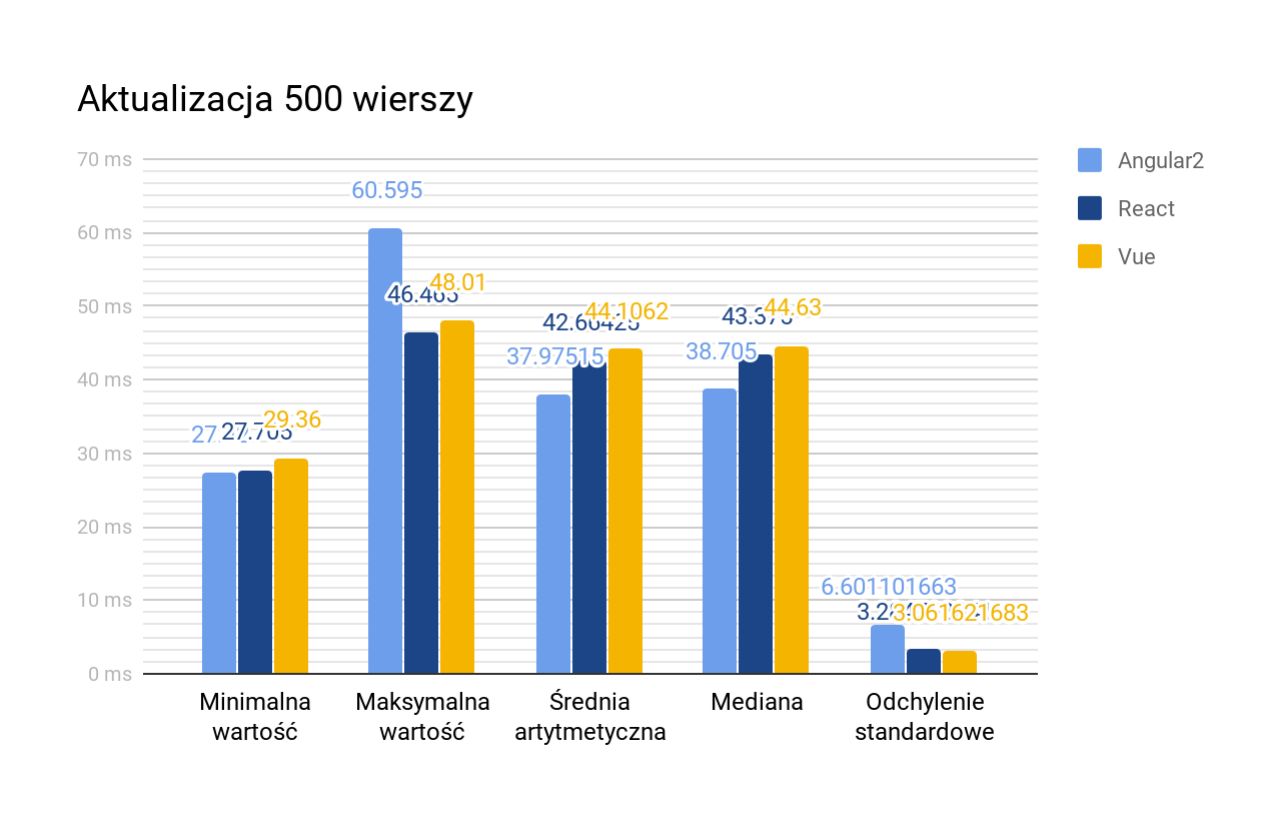
\includegraphics[width=12cm]{rysunek_37.png}
%     \caption{Diagram kolumnowy obrazujący wynik badania pomiaru czasu zmiany wartości dla 500 elementów listy}
%     \label{fig:rysunek_37}
% \end{figure}

% \begin{figure}[!ht]
%     \centering
%     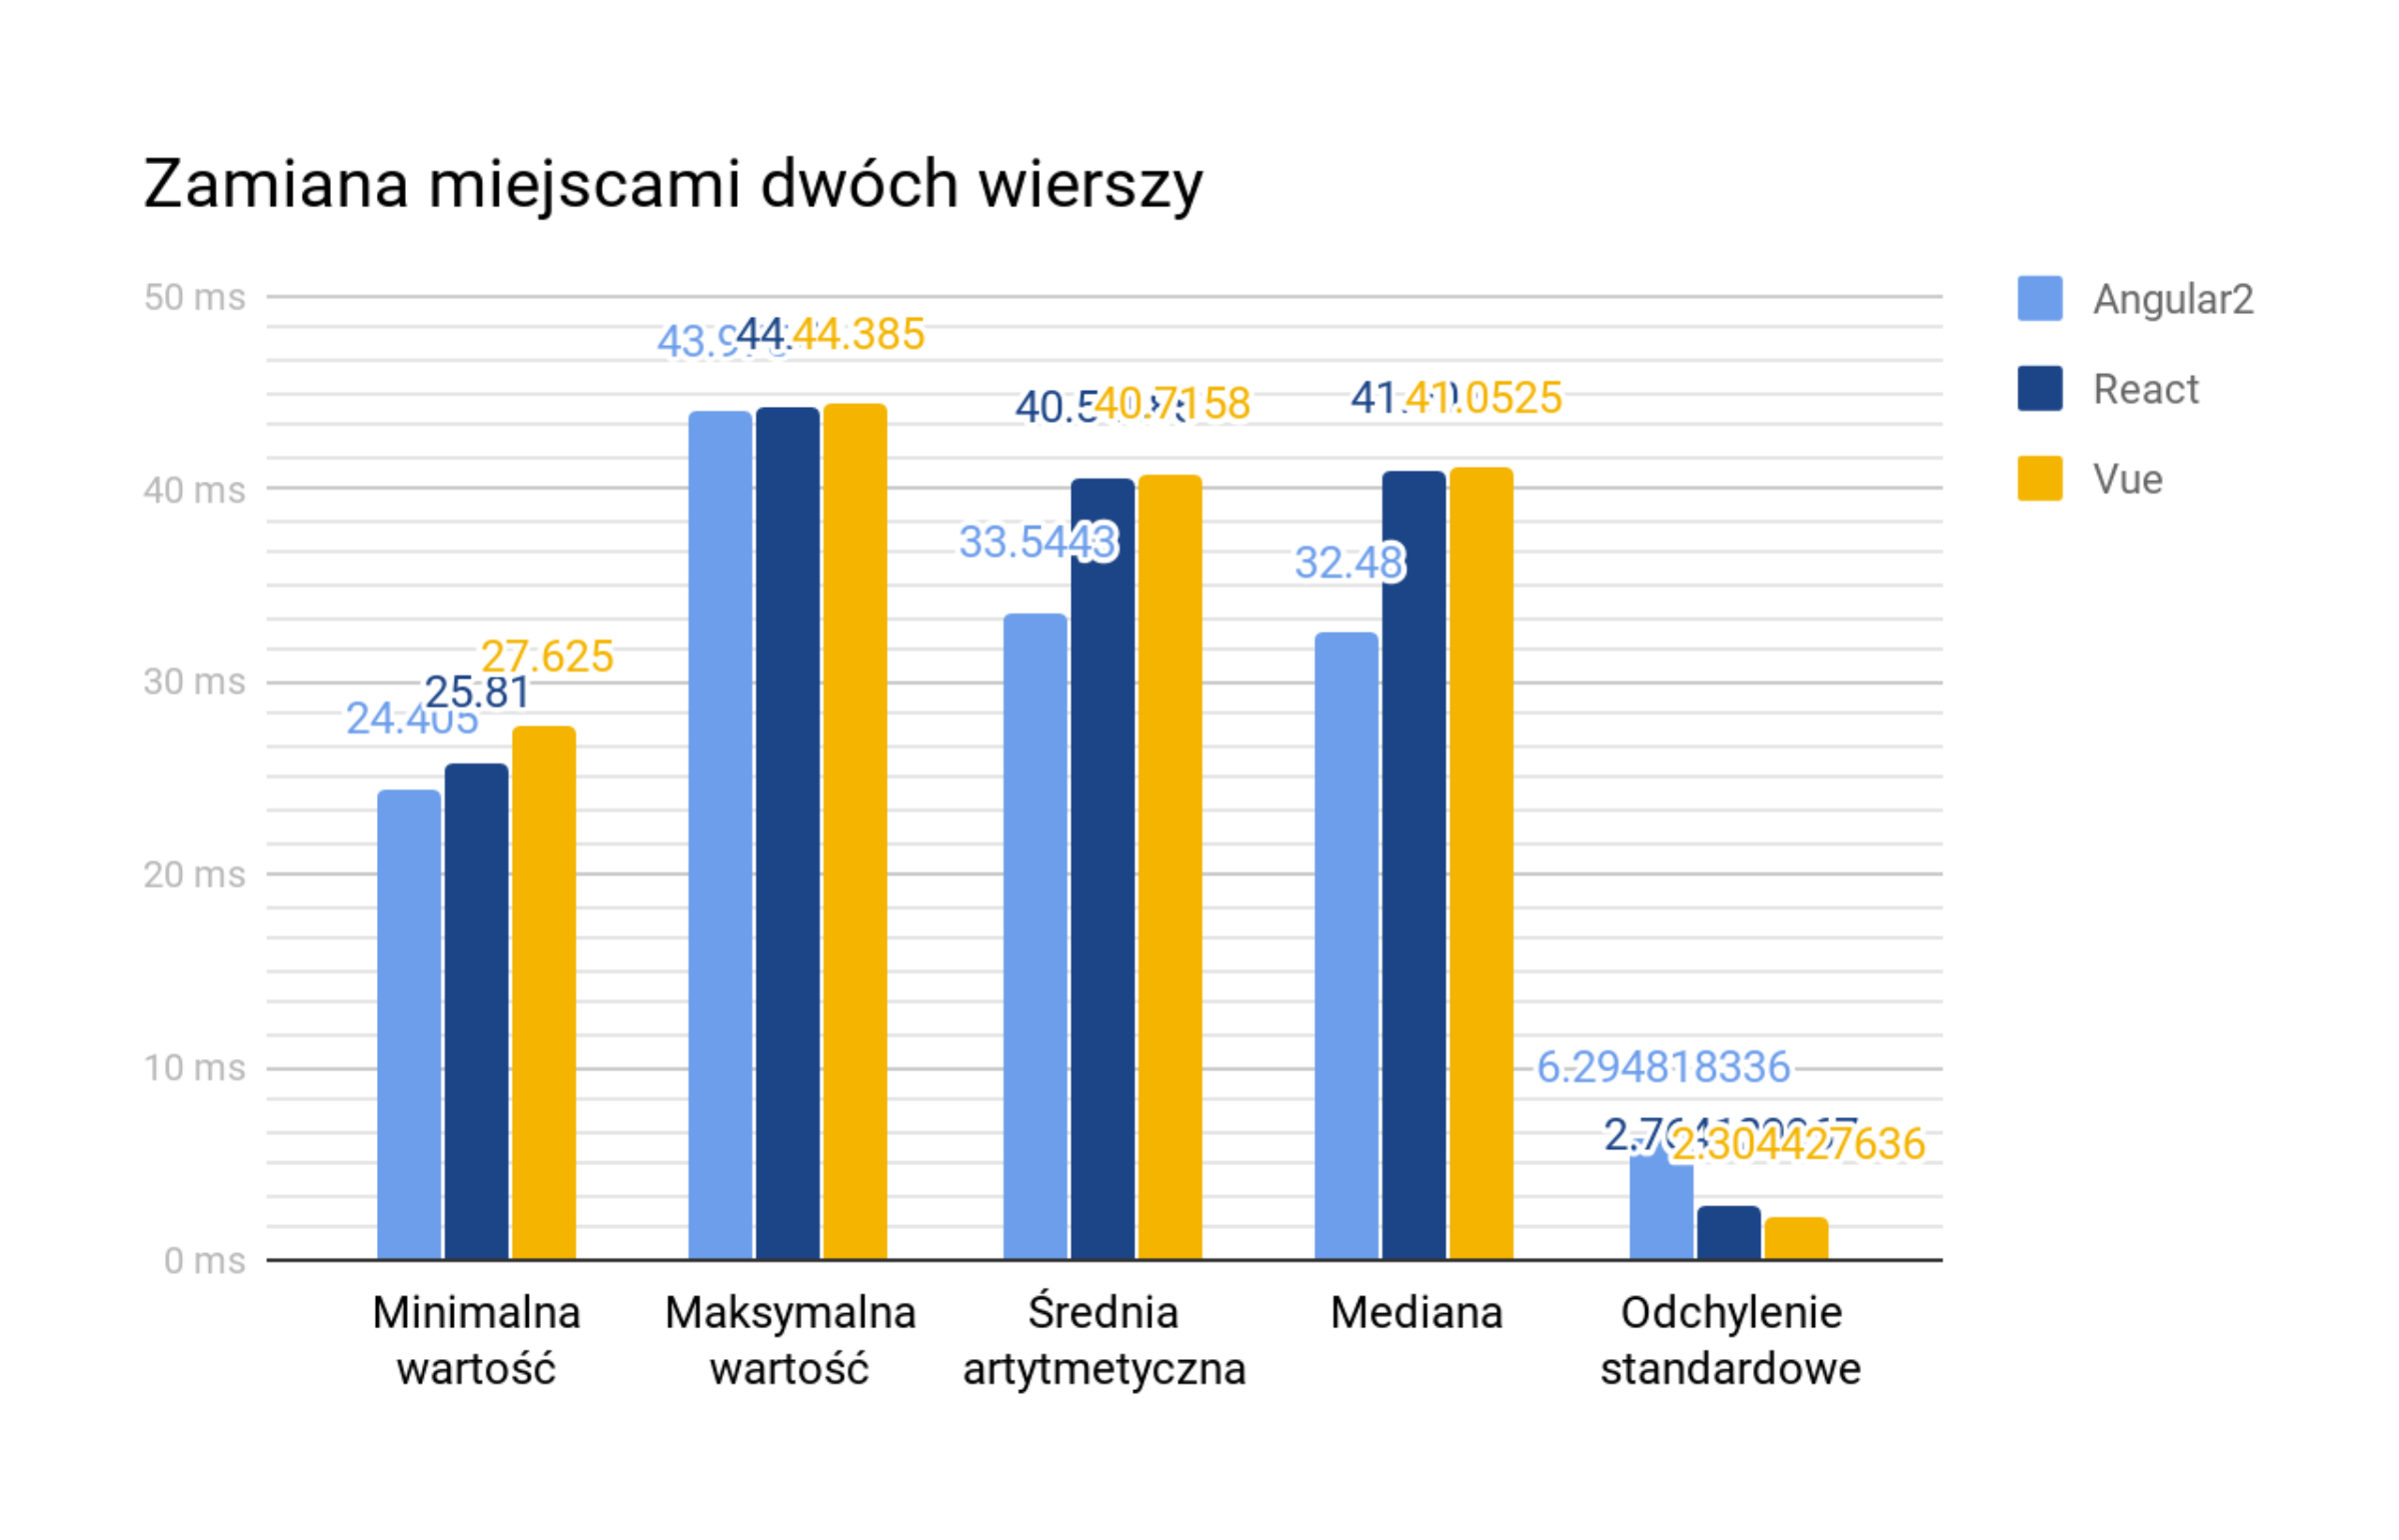
\includegraphics[width=12cm]{rysunek_38.png}
%     \caption{Diagram kolumnowy obrazujący wynik badania pomiaru czasu zamiany miejscami dwóch wartości na liście elementów}
%     \label{fig:rysunek_38}
% \end{figure}

% \begin{figure}[!ht]
%     \centering
%     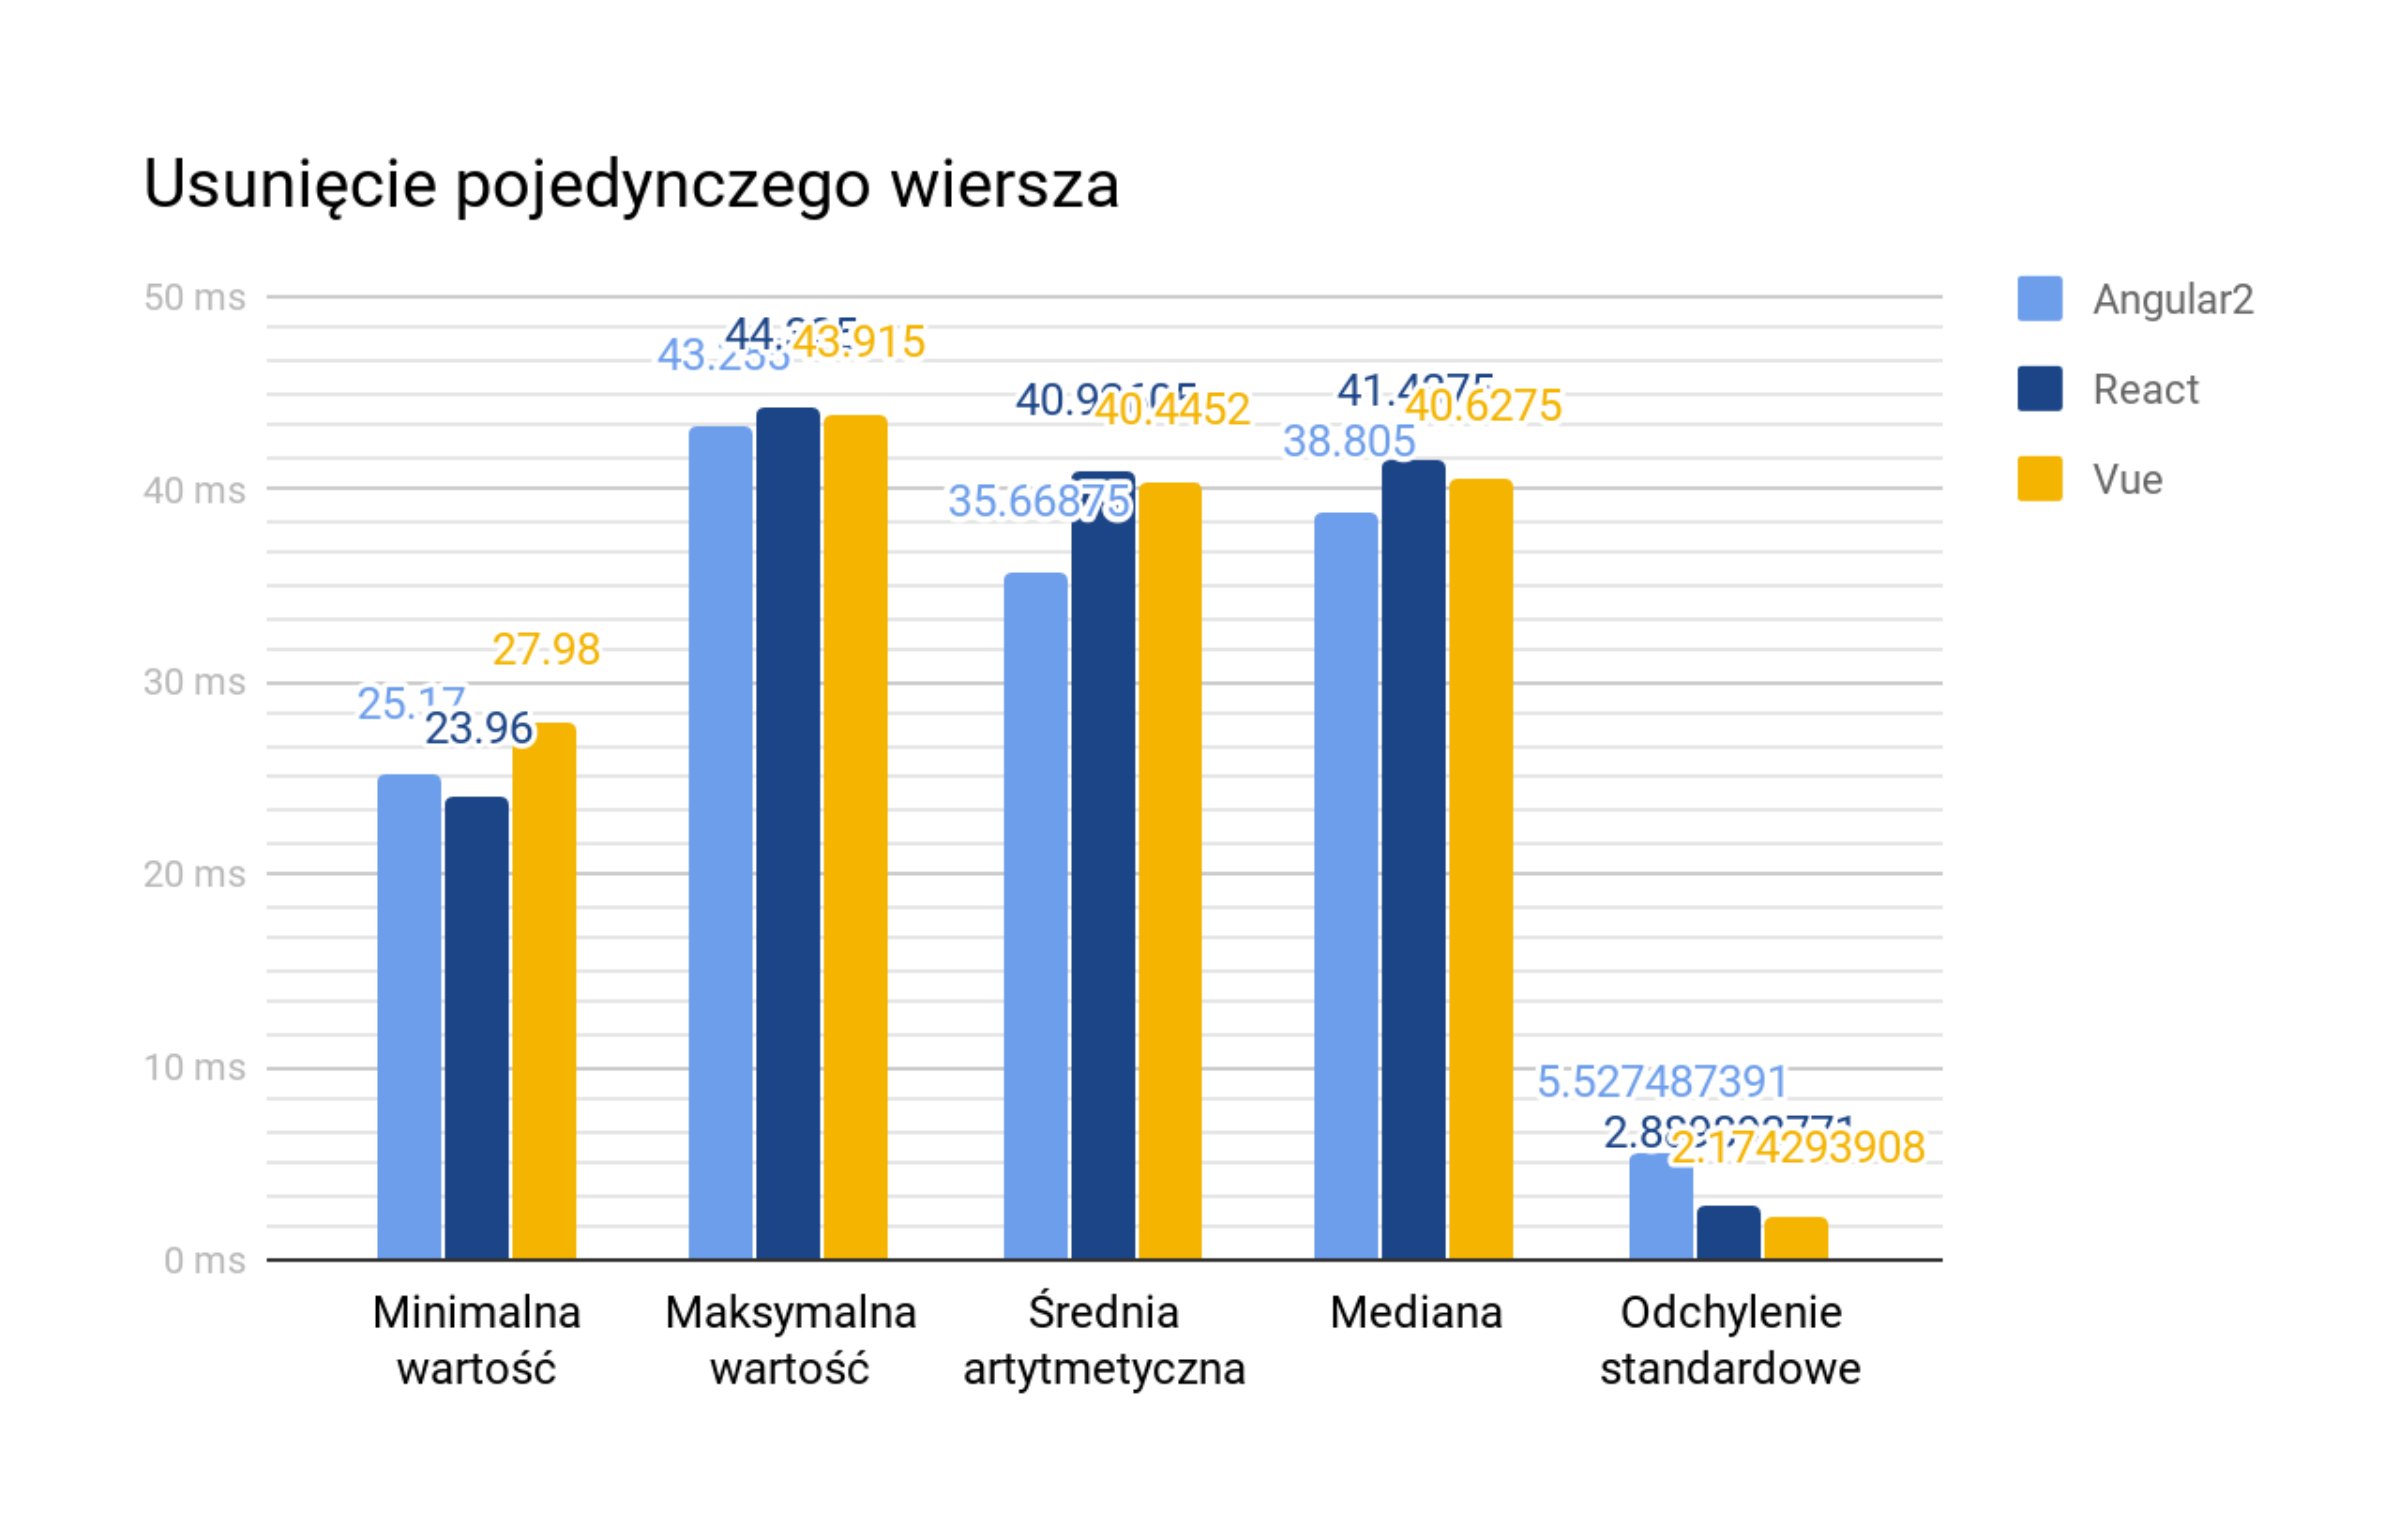
\includegraphics[width=12cm]{rysunek_39.png}
%     \caption{Diagram kolumnowy obrazujący wynik badania pomiaru czasu usunięcia pojedynczej wartości z listy elementów}
%     \label{fig:rysunek_39}
% \end{figure}

% \begin{figure}[!ht]
%     \centering
%     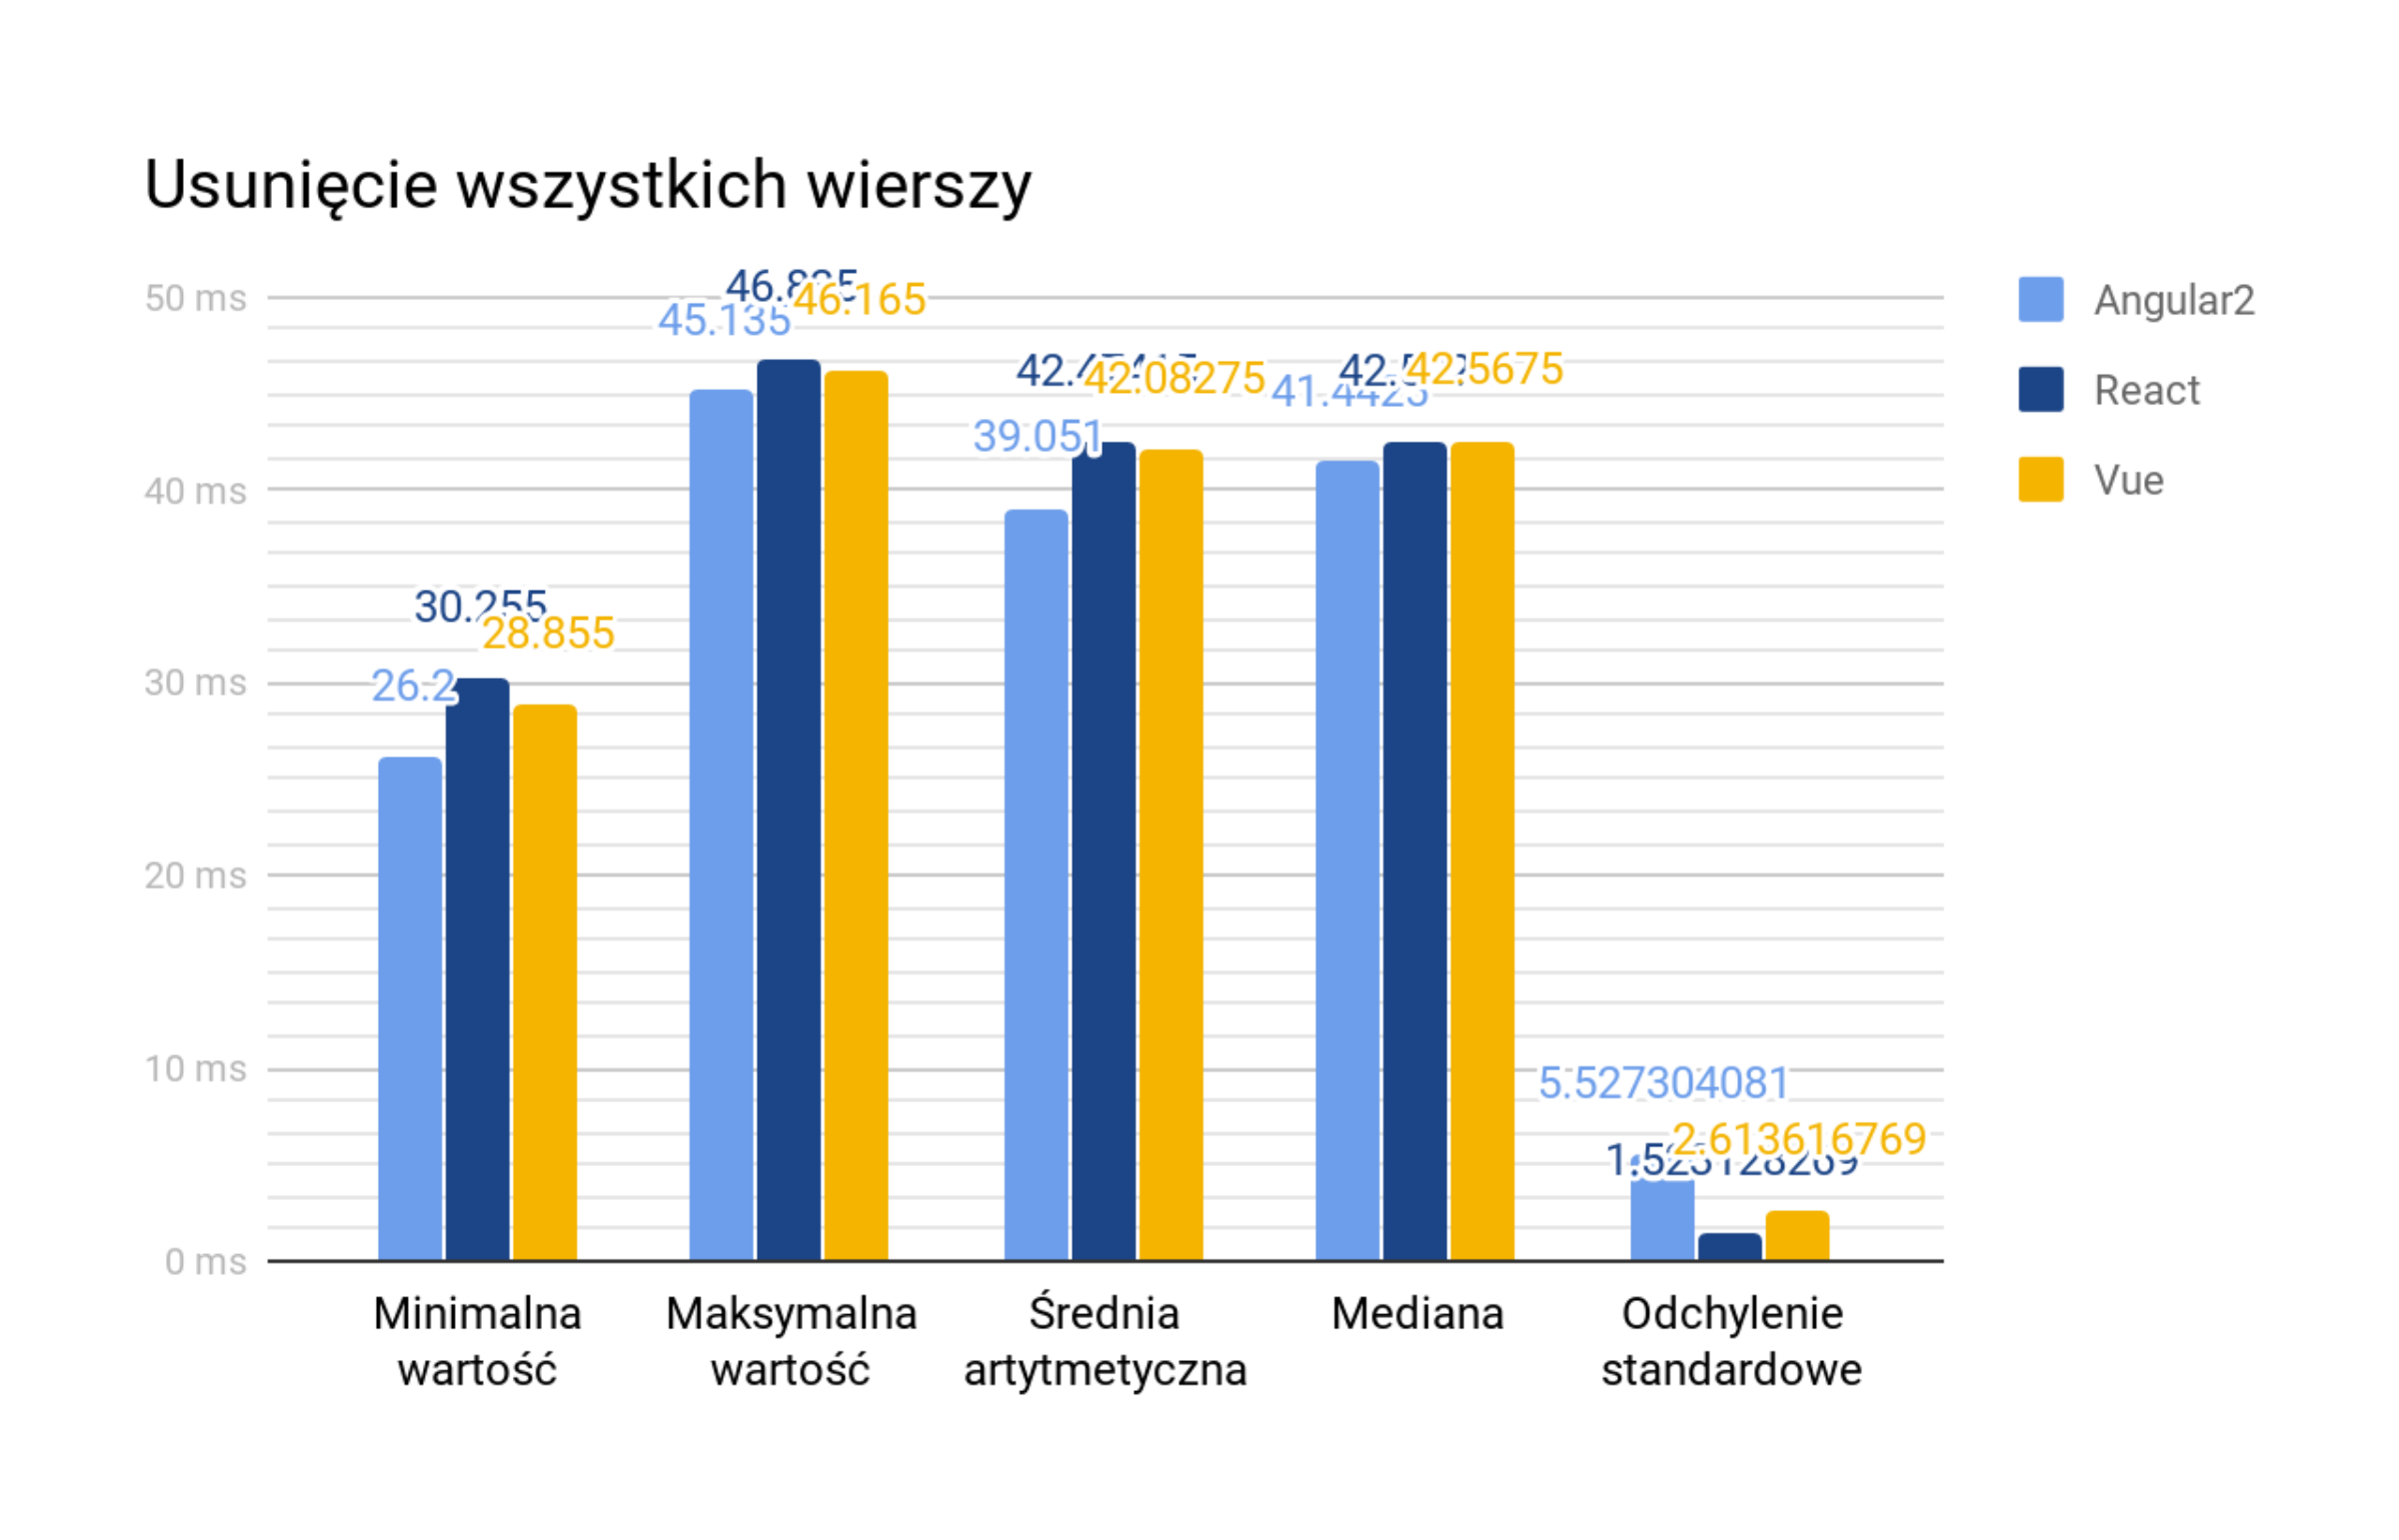
\includegraphics[width=12cm]{rysunek_40.png}
%     \caption{Diagram kolumnowy obrazujący wynik badania pomiaru czasu usunięcia wszystkich wartości z listy elementów}
%     \label{fig:rysunek_40}
% \end{figure}

%czyści puste strony
\let\cleardoublepage\clearpage